\documentclass[twoside]{book}

% Packages required by doxygen
\usepackage{fixltx2e}
\usepackage{calc}
\usepackage{doxygen}
\usepackage{graphicx}
\usepackage[utf8]{inputenc}
\usepackage{makeidx}
\usepackage{multicol}
\usepackage{multirow}
\PassOptionsToPackage{warn}{textcomp}
\usepackage{textcomp}
\usepackage[nointegrals]{wasysym}
\usepackage[table]{xcolor}

% Font selection
\usepackage[T1]{fontenc}
\usepackage{mathptmx}
\usepackage[scaled=.90]{helvet}
\usepackage{courier}
\usepackage{amssymb}
\usepackage{sectsty}
\renewcommand{\familydefault}{\sfdefault}
\allsectionsfont{%
  \fontseries{bc}\selectfont%
  \color{darkgray}%
}
\renewcommand{\DoxyLabelFont}{%
  \fontseries{bc}\selectfont%
  \color{darkgray}%
}
\newcommand{\+}{\discretionary{\mbox{\scriptsize$\hookleftarrow$}}{}{}}

% Page & text layout
\usepackage{geometry}
\geometry{%
  a4paper,%
  top=2.5cm,%
  bottom=2.5cm,%
  left=2.5cm,%
  right=2.5cm%
}
\tolerance=750
\hfuzz=15pt
\hbadness=750
\setlength{\emergencystretch}{15pt}
\setlength{\parindent}{0cm}
\setlength{\parskip}{0.2cm}
\makeatletter
\renewcommand{\paragraph}{%
  \@startsection{paragraph}{4}{0ex}{-1.0ex}{1.0ex}{%
    \normalfont\normalsize\bfseries\SS@parafont%
  }%
}
\renewcommand{\subparagraph}{%
  \@startsection{subparagraph}{5}{0ex}{-1.0ex}{1.0ex}{%
    \normalfont\normalsize\bfseries\SS@subparafont%
  }%
}
\makeatother

% Headers & footers
\usepackage{fancyhdr}
\pagestyle{fancyplain}
\fancyhead[LE]{\fancyplain{}{\bfseries\thepage}}
\fancyhead[CE]{\fancyplain{}{}}
\fancyhead[RE]{\fancyplain{}{\bfseries\leftmark}}
\fancyhead[LO]{\fancyplain{}{\bfseries\rightmark}}
\fancyhead[CO]{\fancyplain{}{}}
\fancyhead[RO]{\fancyplain{}{\bfseries\thepage}}
\fancyfoot[LE]{\fancyplain{}{}}
\fancyfoot[CE]{\fancyplain{}{}}
\fancyfoot[RE]{\fancyplain{}{\bfseries\scriptsize Generated on Sun Nov 30 2014 18\+:00\+:04 for Manuscript-\/vc by Doxygen }}
\fancyfoot[LO]{\fancyplain{}{\bfseries\scriptsize Generated on Sun Nov 30 2014 18\+:00\+:04 for Manuscript-\/vc by Doxygen }}
\fancyfoot[CO]{\fancyplain{}{}}
\fancyfoot[RO]{\fancyplain{}{}}
\renewcommand{\footrulewidth}{0.4pt}
\renewcommand{\chaptermark}[1]{%
  \markboth{#1}{}%
}
\renewcommand{\sectionmark}[1]{%
  \markright{\thesection\ #1}%
}

% Indices & bibliography
\usepackage{natbib}
\usepackage[titles]{tocloft}
\setcounter{tocdepth}{3}
\setcounter{secnumdepth}{5}
\makeindex

% Hyperlinks (required, but should be loaded last)
\usepackage{ifpdf}
\ifpdf
  \usepackage[pdftex,pagebackref=true]{hyperref}
\else
  \usepackage[ps2pdf,pagebackref=true]{hyperref}
\fi
\hypersetup{%
  colorlinks=true,%
  linkcolor=blue,%
  citecolor=blue,%
  unicode%
}

% Custom commands
\newcommand{\clearemptydoublepage}{%
  \newpage{\pagestyle{empty}\cleardoublepage}%
}


%===== C O N T E N T S =====

\begin{document}

% Titlepage & ToC
\hypersetup{pageanchor=false,
             bookmarks=true,
             bookmarksnumbered=true,
             pdfencoding=unicode
            }
\pagenumbering{roman}
\begin{titlepage}
\vspace*{7cm}
\begin{center}%
{\Large Manuscript-\/vc }\\
\vspace*{1cm}
{\large Generated by Doxygen 1.8.8}\\
\vspace*{0.5cm}
{\small Sun Nov 30 2014 18:00:04}\\
\end{center}
\end{titlepage}
\clearemptydoublepage
\tableofcontents
\clearemptydoublepage
\pagenumbering{arabic}
\hypersetup{pageanchor=true}

%--- Begin generated contents ---
\chapter{Namespace Index}
\section{Namespace List}
Here is a list of all namespaces with brief descriptions\+:\begin{DoxyCompactList}
\item\contentsline{section}{\hyperlink{namespace_image_tools}{Image\+Tools} }{\pageref{namespace_image_tools}}{}
\end{DoxyCompactList}

\chapter{Hierarchical Index}
\section{Class Hierarchy}
This inheritance list is sorted roughly, but not completely, alphabetically\+:\begin{DoxyCompactList}
\item \contentsline{section}{Component\+Extractor}{\pageref{class_component_extractor}}{}
\begin{DoxyCompactList}
\item \contentsline{section}{Binary\+Component\+Extractor}{\pageref{class_binary_component_extractor}}{}
\end{DoxyCompactList}
\item \contentsline{section}{Connected\+Component}{\pageref{class_connected_component}}{}
\item \contentsline{section}{Contour}{\pageref{class_contour}}{}
\item \contentsline{section}{D\+Image}{\pageref{class_d_image}}{}
\begin{DoxyCompactList}
\item \contentsline{section}{Page\+Image}{\pageref{class_page_image}}{}
\end{DoxyCompactList}
\item \contentsline{section}{Feature}{\pageref{class_feature}}{}
\begin{DoxyCompactList}
\item \contentsline{section}{Gabor\+Blob\+Feature}{\pageref{class_gabor_blob_feature}}{}
\item \contentsline{section}{Int\+Feature}{\pageref{class_int_feature}}{}
\item \contentsline{section}{Scalar\+Feature$<$ T $>$}{\pageref{class_scalar_feature}}{}
\end{DoxyCompactList}
\item \contentsline{section}{Feature\+Extractor}{\pageref{class_feature_extractor}}{}
\begin{DoxyCompactList}
\item \contentsline{section}{Gabor\+Blob\+Extractor}{\pageref{class_gabor_blob_extractor}}{}
\end{DoxyCompactList}
\item \contentsline{section}{Histogram}{\pageref{class_histogram}}{}
\item \contentsline{section}{Image\+Operator}{\pageref{class_image_operator}}{}
\begin{DoxyCompactList}
\item \contentsline{section}{Image\+Binarizer}{\pageref{class_image_binarizer}}{}
\begin{DoxyCompactList}
\item \contentsline{section}{Global\+Binarizer}{\pageref{class_global_binarizer}}{}
\item \contentsline{section}{Itay\+Binarizer}{\pageref{class_itay_binarizer}}{}
\item \contentsline{section}{Otsu\+Binarizer}{\pageref{class_otsu_binarizer}}{}
\item \contentsline{section}{Otsul\+Binarizer}{\pageref{class_otsul_binarizer}}{}
\item \contentsline{section}{Threshold\+Binarizer}{\pageref{class_threshold_binarizer}}{}
\end{DoxyCompactList}
\item \contentsline{section}{Image\+Converter}{\pageref{class_image_converter}}{}
\item \contentsline{section}{Image\+Enhancer}{\pageref{class_image_enhancer}}{}
\item \contentsline{section}{Image\+Filter}{\pageref{class_image_filter}}{}
\begin{DoxyCompactList}
\item \contentsline{section}{Anisotropic\+Filter}{\pageref{class_anisotropic_filter}}{}
\end{DoxyCompactList}
\item \contentsline{section}{Image\+Projector}{\pageref{class_image_projector}}{}
\begin{DoxyCompactList}
\item \contentsline{section}{Projection\+Profile}{\pageref{class_projection_profile}}{}
\end{DoxyCompactList}
\end{DoxyCompactList}
\item \contentsline{section}{Metric}{\pageref{class_metric}}{}
\begin{DoxyCompactList}
\item \contentsline{section}{Metric\+D\+T\+W}{\pageref{class_metric_d_t_w}}{}
\end{DoxyCompactList}
\item \contentsline{section}{Text\+Line\+Extractor}{\pageref{class_text_line_extractor}}{}
\begin{DoxyCompactList}
\item \contentsline{section}{Profile\+Seam\+Text\+Line\+Extractor}{\pageref{class_profile_seam_text_line_extractor}}{}
\item \contentsline{section}{Rafi\+Text\+Line\+Extractor}{\pageref{class_rafi_text_line_extractor}}{}
\end{DoxyCompactList}
\end{DoxyCompactList}

\chapter{Class Index}
\section{Class List}
Here are the classes, structs, unions and interfaces with brief descriptions\+:\begin{DoxyCompactList}
\item\contentsline{section}{\hyperlink{class_anisotropic_filter}{Anisotropic\+Filter} }{\pageref{class_anisotropic_filter}}{}
\item\contentsline{section}{\hyperlink{class_binary_component_extractor}{Binary\+Component\+Extractor} \\*Binary component extractor class }{\pageref{class_binary_component_extractor}}{}
\item\contentsline{section}{\hyperlink{class_component_extractor}{Component\+Extractor} }{\pageref{class_component_extractor}}{}
\item\contentsline{section}{\hyperlink{class_connected_component}{Connected\+Component} \\*Connected component. }{\pageref{class_connected_component}}{}
\item\contentsline{section}{\hyperlink{class_contour}{Contour} }{\pageref{class_contour}}{}
\item\contentsline{section}{\hyperlink{class_d_image}{D\+Image} }{\pageref{class_d_image}}{}
\item\contentsline{section}{\hyperlink{class_feature}{Feature} }{\pageref{class_feature}}{}
\item\contentsline{section}{\hyperlink{class_feature_extractor}{Feature\+Extractor} }{\pageref{class_feature_extractor}}{}
\item\contentsline{section}{\hyperlink{class_gabor_blob_extractor}{Gabor\+Blob\+Extractor} }{\pageref{class_gabor_blob_extractor}}{}
\item\contentsline{section}{\hyperlink{class_gabor_blob_feature}{Gabor\+Blob\+Feature} }{\pageref{class_gabor_blob_feature}}{}
\item\contentsline{section}{\hyperlink{class_global_binarizer}{Global\+Binarizer} \\*Global binarizer implment a global binarization algorithm }{\pageref{class_global_binarizer}}{}
\item\contentsline{section}{\hyperlink{class_histogram}{Histogram} }{\pageref{class_histogram}}{}
\item\contentsline{section}{\hyperlink{class_image_binarizer}{Image\+Binarizer} }{\pageref{class_image_binarizer}}{}
\item\contentsline{section}{\hyperlink{class_image_converter}{Image\+Converter} }{\pageref{class_image_converter}}{}
\item\contentsline{section}{\hyperlink{class_image_enhancer}{Image\+Enhancer} }{\pageref{class_image_enhancer}}{}
\item\contentsline{section}{\hyperlink{class_image_filter}{Image\+Filter} }{\pageref{class_image_filter}}{}
\item\contentsline{section}{\hyperlink{class_image_operator}{Image\+Operator} }{\pageref{class_image_operator}}{}
\item\contentsline{section}{\hyperlink{class_image_projector}{Image\+Projector} }{\pageref{class_image_projector}}{}
\item\contentsline{section}{\hyperlink{class_int_feature}{Int\+Feature} }{\pageref{class_int_feature}}{}
\item\contentsline{section}{\hyperlink{class_itay_binarizer}{Itay\+Binarizer} \\*Itay binarizer class implements the Itay binarization algorithm }{\pageref{class_itay_binarizer}}{}
\item\contentsline{section}{\hyperlink{class_metric}{Metric} }{\pageref{class_metric}}{}
\item\contentsline{section}{\hyperlink{class_metric_d_t_w}{Metric\+D\+T\+W} }{\pageref{class_metric_d_t_w}}{}
\item\contentsline{section}{\hyperlink{class_otsu_binarizer}{Otsu\+Binarizer} \\*Otsul binarizer class implements the Otsu binarization algorithm }{\pageref{class_otsu_binarizer}}{}
\item\contentsline{section}{\hyperlink{class_otsul_binarizer}{Otsul\+Binarizer} \\*Otsul binarizer class implements the Otsu binarization algorithm }{\pageref{class_otsul_binarizer}}{}
\item\contentsline{section}{\hyperlink{class_page_image}{Page\+Image} }{\pageref{class_page_image}}{}
\item\contentsline{section}{\hyperlink{class_profile_seam_text_line_extractor}{Profile\+Seam\+Text\+Line\+Extractor} }{\pageref{class_profile_seam_text_line_extractor}}{}
\item\contentsline{section}{\hyperlink{class_projection_profile}{Projection\+Profile} }{\pageref{class_projection_profile}}{}
\item\contentsline{section}{\hyperlink{class_rafi_text_line_extractor}{Rafi\+Text\+Line\+Extractor} }{\pageref{class_rafi_text_line_extractor}}{}
\item\contentsline{section}{\hyperlink{class_scalar_feature}{Scalar\+Feature$<$ T $>$} }{\pageref{class_scalar_feature}}{}
\item\contentsline{section}{\hyperlink{class_text_line_extractor}{Text\+Line\+Extractor} \\*Text line extractor is a base class for text line extraction algorithms. Each should implement the virtual funxtion extract }{\pageref{class_text_line_extractor}}{}
\item\contentsline{section}{\hyperlink{class_threshold_binarizer}{Threshold\+Binarizer} }{\pageref{class_threshold_binarizer}}{}
\end{DoxyCompactList}

\chapter{File Index}
\section{File List}
Here is a list of all files with brief descriptions\+:\begin{DoxyCompactList}
\item\contentsline{section}{Manuscript\+App/\hyperlink{anigauss_8h}{anigauss.\+h} }{\pageref{anigauss_8h}}{}
\item\contentsline{section}{Manuscript\+App/\hyperlink{_anisotropic_filter_8cpp}{Anisotropic\+Filter.\+cpp} }{\pageref{_anisotropic_filter_8cpp}}{}
\item\contentsline{section}{Manuscript\+App/\hyperlink{_anisotropic_filter_8h}{Anisotropic\+Filter.\+h} }{\pageref{_anisotropic_filter_8h}}{}
\item\contentsline{section}{Manuscript\+App/\hyperlink{_binary_component_extractor_8cpp}{Binary\+Component\+Extractor.\+cpp} }{\pageref{_binary_component_extractor_8cpp}}{}
\item\contentsline{section}{Manuscript\+App/\hyperlink{_binary_component_extractor_8h}{Binary\+Component\+Extractor.\+h} }{\pageref{_binary_component_extractor_8h}}{}
\item\contentsline{section}{Manuscript\+App/\hyperlink{_component_extractor_8h}{Component\+Extractor.\+h} }{\pageref{_component_extractor_8h}}{}
\item\contentsline{section}{Manuscript\+App/\hyperlink{_connected_component_8cpp}{Connected\+Component.\+cpp} }{\pageref{_connected_component_8cpp}}{}
\item\contentsline{section}{Manuscript\+App/\hyperlink{_connected_component_8h}{Connected\+Component.\+h} }{\pageref{_connected_component_8h}}{}
\item\contentsline{section}{Manuscript\+App/\hyperlink{_contour_8cpp}{Contour.\+cpp} }{\pageref{_contour_8cpp}}{}
\item\contentsline{section}{Manuscript\+App/\hyperlink{_contour_8h}{Contour.\+h} }{\pageref{_contour_8h}}{}
\item\contentsline{section}{Manuscript\+App/\hyperlink{_d_image_8cpp}{D\+Image.\+cpp} }{\pageref{_d_image_8cpp}}{}
\item\contentsline{section}{Manuscript\+App/\hyperlink{_d_image_8h}{D\+Image.\+h} }{\pageref{_d_image_8h}}{}
\item\contentsline{section}{Manuscript\+App/\hyperlink{dllmain_8cpp}{dllmain.\+cpp} }{\pageref{dllmain_8cpp}}{}
\item\contentsline{section}{Manuscript\+App/\hyperlink{_feature_8h}{Feature.\+h} }{\pageref{_feature_8h}}{}
\item\contentsline{section}{Manuscript\+App/\hyperlink{_feature_extractor_8h}{Feature\+Extractor.\+h} }{\pageref{_feature_extractor_8h}}{}
\item\contentsline{section}{Manuscript\+App/\hyperlink{_gabor_blob_extractor_8cpp}{Gabor\+Blob\+Extractor.\+cpp} }{\pageref{_gabor_blob_extractor_8cpp}}{}
\item\contentsline{section}{Manuscript\+App/\hyperlink{_gabor_blob_extractor_8h}{Gabor\+Blob\+Extractor.\+h} }{\pageref{_gabor_blob_extractor_8h}}{}
\item\contentsline{section}{Manuscript\+App/\hyperlink{_gabor_blob_feature_8cpp}{Gabor\+Blob\+Feature.\+cpp} }{\pageref{_gabor_blob_feature_8cpp}}{}
\item\contentsline{section}{Manuscript\+App/\hyperlink{_gabor_blob_feature_8h}{Gabor\+Blob\+Feature.\+h} }{\pageref{_gabor_blob_feature_8h}}{}
\item\contentsline{section}{Manuscript\+App/\hyperlink{_global_binarizer_8cpp}{Global\+Binarizer.\+cpp} }{\pageref{_global_binarizer_8cpp}}{}
\item\contentsline{section}{Manuscript\+App/\hyperlink{_global_binarizer_8h}{Global\+Binarizer.\+h} }{\pageref{_global_binarizer_8h}}{}
\item\contentsline{section}{Manuscript\+App/\hyperlink{_histogram_8cpp}{Histogram.\+cpp} }{\pageref{_histogram_8cpp}}{}
\item\contentsline{section}{Manuscript\+App/\hyperlink{_histogram_8h}{Histogram.\+h} }{\pageref{_histogram_8h}}{}
\item\contentsline{section}{Manuscript\+App/\hyperlink{_image_binarizer_8h}{Image\+Binarizer.\+h} }{\pageref{_image_binarizer_8h}}{}
\item\contentsline{section}{Manuscript\+App/\hyperlink{_image_converter_8cpp}{Image\+Converter.\+cpp} }{\pageref{_image_converter_8cpp}}{}
\item\contentsline{section}{Manuscript\+App/\hyperlink{_image_converter_8h}{Image\+Converter.\+h} }{\pageref{_image_converter_8h}}{}
\item\contentsline{section}{Manuscript\+App/\hyperlink{_image_enhancer_8h}{Image\+Enhancer.\+h} }{\pageref{_image_enhancer_8h}}{}
\item\contentsline{section}{Manuscript\+App/\hyperlink{_image_filter_8h}{Image\+Filter.\+h} }{\pageref{_image_filter_8h}}{}
\item\contentsline{section}{Manuscript\+App/\hyperlink{_image_operator_8h}{Image\+Operator.\+h} }{\pageref{_image_operator_8h}}{}
\item\contentsline{section}{Manuscript\+App/\hyperlink{_image_projector_8h}{Image\+Projector.\+h} }{\pageref{_image_projector_8h}}{}
\item\contentsline{section}{Manuscript\+App/\hyperlink{_image_tools_8cpp}{Image\+Tools.\+cpp} }{\pageref{_image_tools_8cpp}}{}
\item\contentsline{section}{Manuscript\+App/\hyperlink{_image_tools_8h}{Image\+Tools.\+h} }{\pageref{_image_tools_8h}}{}
\item\contentsline{section}{Manuscript\+App/\hyperlink{_int_feature_8cpp}{Int\+Feature.\+cpp} }{\pageref{_int_feature_8cpp}}{}
\item\contentsline{section}{Manuscript\+App/\hyperlink{_int_feature_8h}{Int\+Feature.\+h} }{\pageref{_int_feature_8h}}{}
\item\contentsline{section}{Manuscript\+App/\hyperlink{_itay_binarizer_8cpp}{Itay\+Binarizer.\+cpp} }{\pageref{_itay_binarizer_8cpp}}{}
\item\contentsline{section}{Manuscript\+App/\hyperlink{_itay_binarizer_8h}{Itay\+Binarizer.\+h} }{\pageref{_itay_binarizer_8h}}{}
\item\contentsline{section}{Manuscript\+App/\hyperlink{_manuscript_8cpp}{Manuscript.\+cpp} }{\pageref{_manuscript_8cpp}}{}
\item\contentsline{section}{Manuscript\+App/\hyperlink{_manuscript_app_8cpp}{Manuscript\+App.\+cpp} }{\pageref{_manuscript_app_8cpp}}{}
\item\contentsline{section}{Manuscript\+App/\hyperlink{_metric_8h}{Metric.\+h} }{\pageref{_metric_8h}}{}
\item\contentsline{section}{Manuscript\+App/\hyperlink{_metric_d_t_w_8cpp}{Metric\+D\+T\+W.\+cpp} }{\pageref{_metric_d_t_w_8cpp}}{}
\item\contentsline{section}{Manuscript\+App/\hyperlink{_metric_d_t_w_8h}{Metric\+D\+T\+W.\+h} }{\pageref{_metric_d_t_w_8h}}{}
\item\contentsline{section}{Manuscript\+App/\hyperlink{_otsu_binarizer_8cpp}{Otsu\+Binarizer.\+cpp} }{\pageref{_otsu_binarizer_8cpp}}{}
\item\contentsline{section}{Manuscript\+App/\hyperlink{_otsu_binarizer_8h}{Otsu\+Binarizer.\+h} }{\pageref{_otsu_binarizer_8h}}{}
\item\contentsline{section}{Manuscript\+App/\hyperlink{_otsul_binarizer_8cpp}{Otsul\+Binarizer.\+cpp} }{\pageref{_otsul_binarizer_8cpp}}{}
\item\contentsline{section}{Manuscript\+App/\hyperlink{_otsul_binarizer_8h}{Otsul\+Binarizer.\+h} }{\pageref{_otsul_binarizer_8h}}{}
\item\contentsline{section}{Manuscript\+App/\hyperlink{_page_image_8cpp}{Page\+Image.\+cpp} }{\pageref{_page_image_8cpp}}{}
\item\contentsline{section}{Manuscript\+App/\hyperlink{_page_image_8h}{Page\+Image.\+h} }{\pageref{_page_image_8h}}{}
\item\contentsline{section}{Manuscript\+App/\hyperlink{_profile_seam_text_line_extractor_8cpp}{Profile\+Seam\+Text\+Line\+Extractor.\+cpp} }{\pageref{_profile_seam_text_line_extractor_8cpp}}{}
\item\contentsline{section}{Manuscript\+App/\hyperlink{_profile_seam_text_line_extractor_8h}{Profile\+Seam\+Text\+Line\+Extractor.\+h} }{\pageref{_profile_seam_text_line_extractor_8h}}{}
\item\contentsline{section}{Manuscript\+App/\hyperlink{_projection_profile_8cpp}{Projection\+Profile.\+cpp} }{\pageref{_projection_profile_8cpp}}{}
\item\contentsline{section}{Manuscript\+App/\hyperlink{_projection_profile_8h}{Projection\+Profile.\+h} }{\pageref{_projection_profile_8h}}{}
\item\contentsline{section}{Manuscript\+App/\hyperlink{_rafi_text_line_extractor_8cpp}{Rafi\+Text\+Line\+Extractor.\+cpp} }{\pageref{_rafi_text_line_extractor_8cpp}}{}
\item\contentsline{section}{Manuscript\+App/\hyperlink{_rafi_text_line_extractor_8h}{Rafi\+Text\+Line\+Extractor.\+h} }{\pageref{_rafi_text_line_extractor_8h}}{}
\item\contentsline{section}{Manuscript\+App/\hyperlink{_scalar_feature_8h}{Scalar\+Feature.\+h} }{\pageref{_scalar_feature_8h}}{}
\item\contentsline{section}{Manuscript\+App/\hyperlink{stdafx_8cpp}{stdafx.\+cpp} }{\pageref{stdafx_8cpp}}{}
\item\contentsline{section}{Manuscript\+App/\hyperlink{stdafx_8h}{stdafx.\+h} }{\pageref{stdafx_8h}}{}
\item\contentsline{section}{Manuscript\+App/\hyperlink{targetver_8h}{targetver.\+h} }{\pageref{targetver_8h}}{}
\item\contentsline{section}{Manuscript\+App/\hyperlink{_text_line_extractor_8h}{Text\+Line\+Extractor.\+h} }{\pageref{_text_line_extractor_8h}}{}
\item\contentsline{section}{Manuscript\+App/\hyperlink{_threshold_binarizer_8cpp}{Threshold\+Binarizer.\+cpp} }{\pageref{_threshold_binarizer_8cpp}}{}
\item\contentsline{section}{Manuscript\+App/\hyperlink{_threshold_binarizer_8h}{Threshold\+Binarizer.\+h} }{\pageref{_threshold_binarizer_8h}}{}
\item\contentsline{section}{Manuscript\+App/\hyperlink{_tools_8h}{Tools.\+h} }{\pageref{_tools_8h}}{}
\end{DoxyCompactList}

\chapter{Namespace Documentation}
\hypertarget{namespace_image_tools}{\section{Image\+Tools Namespace Reference}
\label{namespace_image_tools}\index{Image\+Tools@{Image\+Tools}}
}
\subsection*{Typedefs}
\begin{DoxyCompactItemize}
\item 
typedef std\+::pair$<$ cv\+::\+Point2f, \\*
cv\+::\+Point2f $>$ \hyperlink{namespace_image_tools_ab9b6e111b7139dcff8b2b04b0f36d1a1}{Orientation}
\end{DoxyCompactItemize}
\subsection*{Functions}
\begin{DoxyCompactItemize}
\item 
cv\+::\+Point2f \hyperlink{namespace_image_tools_aef9fa361958e089c60e33af0e1ae96c4}{center\+Of\+Mass} (cv\+::\+Mat mat)
\item 
cv\+::\+Mat \hyperlink{namespace_image_tools_aef7ccc5ec3cb576256506b6539f5ad6e}{variance\+Around\+Point} (cv\+::\+Mat m, cv\+::\+Point2f point)
\item 
\hyperlink{namespace_image_tools_ab9b6e111b7139dcff8b2b04b0f36d1a1}{Orientation} \hyperlink{namespace_image_tools_ab6bb0f737969195fcfceb4723bf474ea}{orientation} (cv\+::\+Mat m, cv\+::\+Point2f \&com)
\item 
void \hyperlink{namespace_image_tools_af76b41d3be28c818faf2a9ec1e3d3bb1}{smooth\+Column} (cv\+::\+Mat mat, cv\+::\+Mat filter, int col\+\_\+idx)
\item 
void \hyperlink{namespace_image_tools_a45492e740afde5d3482a71d5cee9842b}{display} (String win, \hyperlink{class_d_image}{D\+Image} \&img)
\item 
void \hyperlink{namespace_image_tools_a00f243162ed9b7c3dc16d105425e473d}{display} (String win, Mat \&img)
\end{DoxyCompactItemize}


\subsection{Typedef Documentation}
\hypertarget{namespace_image_tools_ab9b6e111b7139dcff8b2b04b0f36d1a1}{\index{Image\+Tools@{Image\+Tools}!Orientation@{Orientation}}
\index{Orientation@{Orientation}!Image\+Tools@{Image\+Tools}}
\subsubsection[{Orientation}]{\setlength{\rightskip}{0pt plus 5cm}typedef std\+::pair$<$cv\+::\+Point2f, cv\+::\+Point2f$>$ {\bf Image\+Tools\+::\+Orientation}}}\label{namespace_image_tools_ab9b6e111b7139dcff8b2b04b0f36d1a1}


\subsection{Function Documentation}
\hypertarget{namespace_image_tools_aef9fa361958e089c60e33af0e1ae96c4}{\index{Image\+Tools@{Image\+Tools}!center\+Of\+Mass@{center\+Of\+Mass}}
\index{center\+Of\+Mass@{center\+Of\+Mass}!Image\+Tools@{Image\+Tools}}
\subsubsection[{center\+Of\+Mass}]{\setlength{\rightskip}{0pt plus 5cm}cv\+::\+Point2f Image\+Tools\+::center\+Of\+Mass (
\begin{DoxyParamCaption}
\item[{cv\+::\+Mat}]{mat}
\end{DoxyParamCaption}
)}}\label{namespace_image_tools_aef9fa361958e089c60e33af0e1ae96c4}
\hypertarget{namespace_image_tools_a45492e740afde5d3482a71d5cee9842b}{\index{Image\+Tools@{Image\+Tools}!display@{display}}
\index{display@{display}!Image\+Tools@{Image\+Tools}}
\subsubsection[{display}]{\setlength{\rightskip}{0pt plus 5cm}void Image\+Tools\+::display (
\begin{DoxyParamCaption}
\item[{String}]{win, }
\item[{{\bf D\+Image} \&}]{img}
\end{DoxyParamCaption}
)}}\label{namespace_image_tools_a45492e740afde5d3482a71d5cee9842b}
\hypertarget{namespace_image_tools_a00f243162ed9b7c3dc16d105425e473d}{\index{Image\+Tools@{Image\+Tools}!display@{display}}
\index{display@{display}!Image\+Tools@{Image\+Tools}}
\subsubsection[{display}]{\setlength{\rightskip}{0pt plus 5cm}void Image\+Tools\+::display (
\begin{DoxyParamCaption}
\item[{String}]{win, }
\item[{Mat \&}]{img}
\end{DoxyParamCaption}
)}}\label{namespace_image_tools_a00f243162ed9b7c3dc16d105425e473d}
\hypertarget{namespace_image_tools_ab6bb0f737969195fcfceb4723bf474ea}{\index{Image\+Tools@{Image\+Tools}!orientation@{orientation}}
\index{orientation@{orientation}!Image\+Tools@{Image\+Tools}}
\subsubsection[{orientation}]{\setlength{\rightskip}{0pt plus 5cm}{\bf Image\+Tools\+::\+Orientation} Image\+Tools\+::orientation (
\begin{DoxyParamCaption}
\item[{cv\+::\+Mat}]{m, }
\item[{cv\+::\+Point2f \&}]{com}
\end{DoxyParamCaption}
)}}\label{namespace_image_tools_ab6bb0f737969195fcfceb4723bf474ea}
\hypertarget{namespace_image_tools_af76b41d3be28c818faf2a9ec1e3d3bb1}{\index{Image\+Tools@{Image\+Tools}!smooth\+Column@{smooth\+Column}}
\index{smooth\+Column@{smooth\+Column}!Image\+Tools@{Image\+Tools}}
\subsubsection[{smooth\+Column}]{\setlength{\rightskip}{0pt plus 5cm}void Image\+Tools\+::smooth\+Column (
\begin{DoxyParamCaption}
\item[{cv\+::\+Mat}]{mat, }
\item[{cv\+::\+Mat}]{filter, }
\item[{int}]{col\+\_\+idx}
\end{DoxyParamCaption}
)}}\label{namespace_image_tools_af76b41d3be28c818faf2a9ec1e3d3bb1}
\hypertarget{namespace_image_tools_aef7ccc5ec3cb576256506b6539f5ad6e}{\index{Image\+Tools@{Image\+Tools}!variance\+Around\+Point@{variance\+Around\+Point}}
\index{variance\+Around\+Point@{variance\+Around\+Point}!Image\+Tools@{Image\+Tools}}
\subsubsection[{variance\+Around\+Point}]{\setlength{\rightskip}{0pt plus 5cm}cv\+::\+Mat Image\+Tools\+::variance\+Around\+Point (
\begin{DoxyParamCaption}
\item[{cv\+::\+Mat}]{m, }
\item[{cv\+::\+Point2f}]{point}
\end{DoxyParamCaption}
)}}\label{namespace_image_tools_aef7ccc5ec3cb576256506b6539f5ad6e}

\chapter{Class Documentation}
\hypertarget{class_anisotropic_filter}{\section{Anisotropic\+Filter Class Reference}
\label{class_anisotropic_filter}\index{Anisotropic\+Filter@{Anisotropic\+Filter}}
}


{\ttfamily \#include $<$Anisotropic\+Filter.\+h$>$}

Inheritance diagram for Anisotropic\+Filter\+:\begin{figure}[H]
\begin{center}
\leavevmode
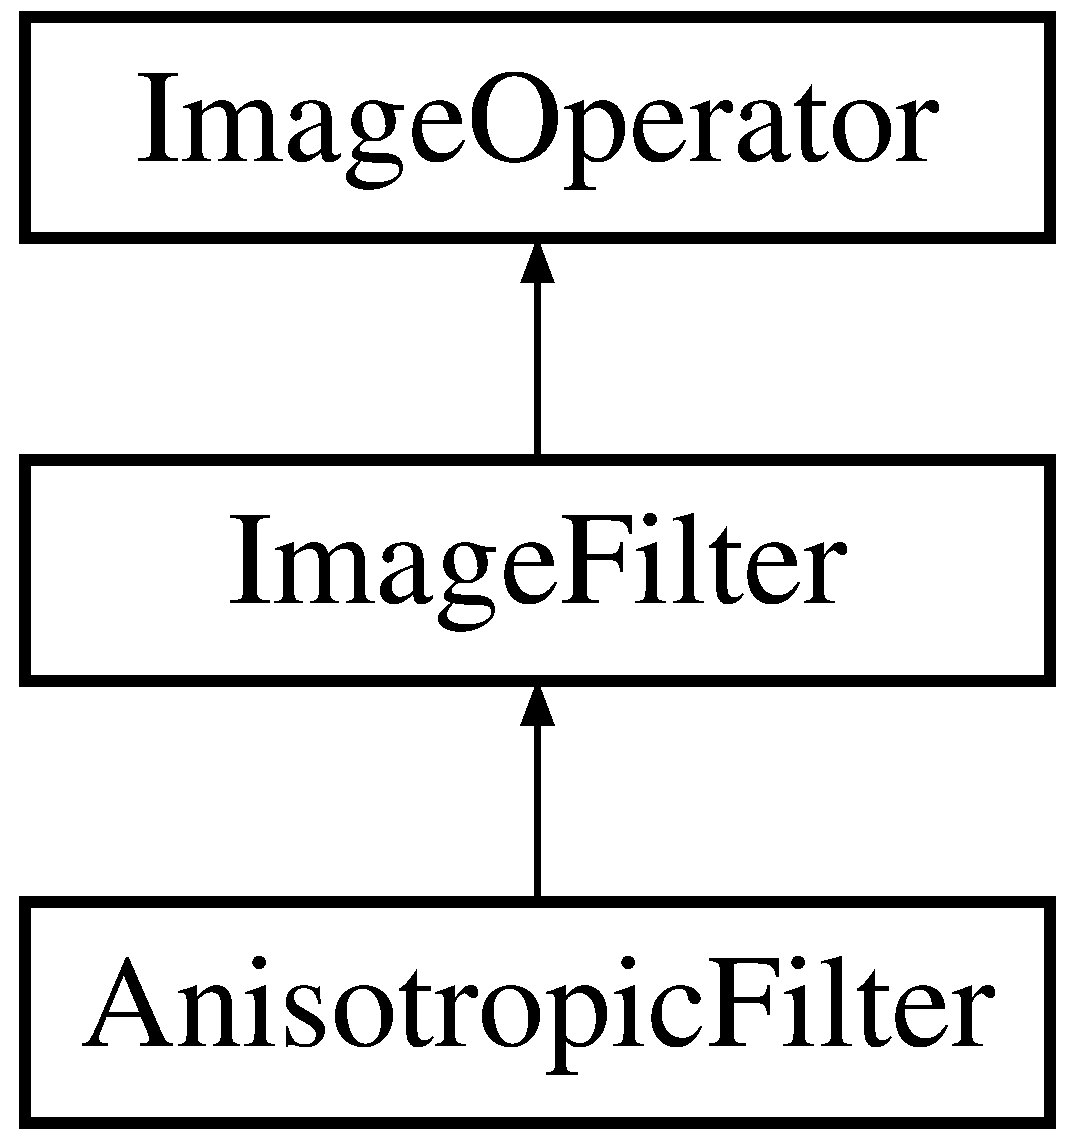
\includegraphics[height=3.000000cm]{class_anisotropic_filter}
\end{center}
\end{figure}
\subsection*{Public Member Functions}
\begin{DoxyCompactItemize}
\item 
\hyperlink{class_anisotropic_filter_ae47e28a13ee052b05d173cf6abd9975c}{Anisotropic\+Filter} ()
\item 
\hyperlink{class_d_image}{D\+Image} $\ast$ \hyperlink{class_anisotropic_filter_addbceed7b786a575f553bd4a41e0987c}{filter} ()
\end{DoxyCompactItemize}
\subsection*{Additional Inherited Members}


\subsection{Constructor \& Destructor Documentation}
\hypertarget{class_anisotropic_filter_ae47e28a13ee052b05d173cf6abd9975c}{\index{Anisotropic\+Filter@{Anisotropic\+Filter}!Anisotropic\+Filter@{Anisotropic\+Filter}}
\index{Anisotropic\+Filter@{Anisotropic\+Filter}!Anisotropic\+Filter@{Anisotropic\+Filter}}
\subsubsection[{Anisotropic\+Filter}]{\setlength{\rightskip}{0pt plus 5cm}Anisotropic\+Filter\+::\+Anisotropic\+Filter (
\begin{DoxyParamCaption}
{}
\end{DoxyParamCaption}
)}}\label{class_anisotropic_filter_ae47e28a13ee052b05d173cf6abd9975c}


\subsection{Member Function Documentation}
\hypertarget{class_anisotropic_filter_addbceed7b786a575f553bd4a41e0987c}{\index{Anisotropic\+Filter@{Anisotropic\+Filter}!filter@{filter}}
\index{filter@{filter}!Anisotropic\+Filter@{Anisotropic\+Filter}}
\subsubsection[{filter}]{\setlength{\rightskip}{0pt plus 5cm}{\bf D\+Image} $\ast$ Anisotropic\+Filter\+::filter (
\begin{DoxyParamCaption}
{}
\end{DoxyParamCaption}
)\hspace{0.3cm}{\ttfamily [virtual]}}}\label{class_anisotropic_filter_addbceed7b786a575f553bd4a41e0987c}


Implements \hyperlink{class_image_filter_afb06f41ef9470e2e2673eb3481c1f86a}{Image\+Filter}.



The documentation for this class was generated from the following files\+:\begin{DoxyCompactItemize}
\item 
Manuscript\+App/\hyperlink{_anisotropic_filter_8h}{Anisotropic\+Filter.\+h}\item 
Manuscript\+App/\hyperlink{_anisotropic_filter_8cpp}{Anisotropic\+Filter.\+cpp}\end{DoxyCompactItemize}

\hypertarget{class_binary_component_extractor}{\section{Binary\+Component\+Extractor Class Reference}
\label{class_binary_component_extractor}\index{Binary\+Component\+Extractor@{Binary\+Component\+Extractor}}
}


Binary component extractor class  




{\ttfamily \#include $<$Binary\+Component\+Extractor.\+h$>$}

Inheritance diagram for Binary\+Component\+Extractor\+:\begin{figure}[H]
\begin{center}
\leavevmode
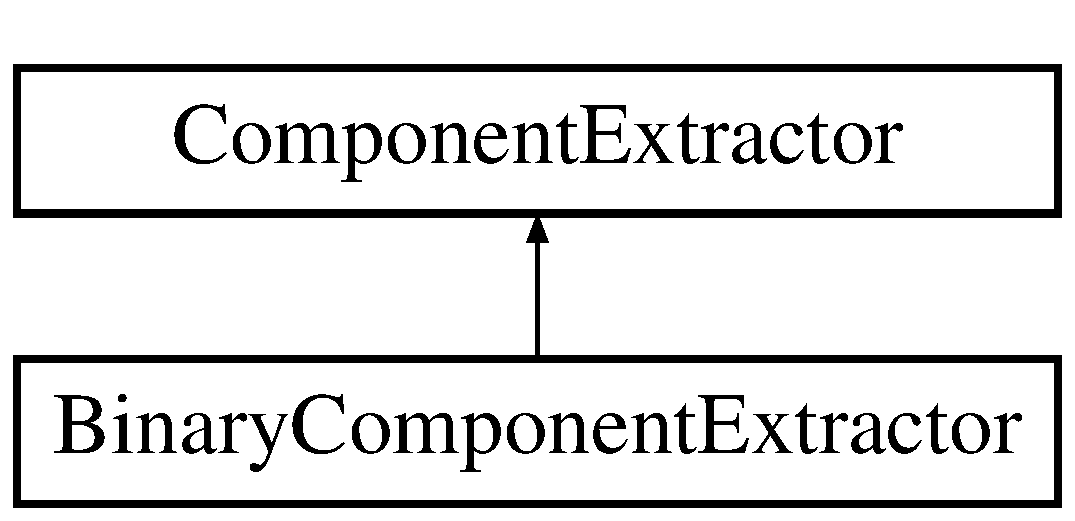
\includegraphics[height=2.000000cm]{class_binary_component_extractor}
\end{center}
\end{figure}
\subsection*{Public Member Functions}
\begin{DoxyCompactItemize}
\item 
\hyperlink{class_binary_component_extractor_ab350a4d29003655c652d7e7943e7854e}{Binary\+Component\+Extractor} (void)
\item 
\hyperlink{class_binary_component_extractor_aa1be60410fd2e11b1bedfeac3bb44519}{$\sim$\+Binary\+Component\+Extractor} (void)
\item 
void \hyperlink{class_binary_component_extractor_a675e103667b7eeb343765c0daa5686a5}{collect\+Components} (vector$<$ vector$<$ Point $>$$>$ \&contours, vector$<$ Vec4i $>$ hierarchy, vector$<$ \hyperlink{class_connected_component}{Connected\+Component} $\ast$ $>$ \&component)
\begin{DoxyCompactList}\small\item\em Collect components. \end{DoxyCompactList}\item 
void \hyperlink{class_binary_component_extractor_a16232815f3a3e8e28fd80a733ff71383}{extract} (vector$<$ \hyperlink{class_connected_component}{Connected\+Component} $\ast$ $>$ \&)
\begin{DoxyCompactList}\small\item\em Extracts the given components. \end{DoxyCompactList}\end{DoxyCompactItemize}
\subsection*{Additional Inherited Members}


\subsection{Detailed Description}
Binary component extractor class 

El Sana, 2/15/2012. 

\subsection{Constructor \& Destructor Documentation}
\hypertarget{class_binary_component_extractor_ab350a4d29003655c652d7e7943e7854e}{\index{Binary\+Component\+Extractor@{Binary\+Component\+Extractor}!Binary\+Component\+Extractor@{Binary\+Component\+Extractor}}
\index{Binary\+Component\+Extractor@{Binary\+Component\+Extractor}!Binary\+Component\+Extractor@{Binary\+Component\+Extractor}}
\subsubsection[{Binary\+Component\+Extractor}]{\setlength{\rightskip}{0pt plus 5cm}Binary\+Component\+Extractor\+::\+Binary\+Component\+Extractor (
\begin{DoxyParamCaption}
\item[{void}]{}
\end{DoxyParamCaption}
)\hspace{0.3cm}{\ttfamily [inline]}}}\label{class_binary_component_extractor_ab350a4d29003655c652d7e7943e7854e}
\hypertarget{class_binary_component_extractor_aa1be60410fd2e11b1bedfeac3bb44519}{\index{Binary\+Component\+Extractor@{Binary\+Component\+Extractor}!````~Binary\+Component\+Extractor@{$\sim$\+Binary\+Component\+Extractor}}
\index{````~Binary\+Component\+Extractor@{$\sim$\+Binary\+Component\+Extractor}!Binary\+Component\+Extractor@{Binary\+Component\+Extractor}}
\subsubsection[{$\sim$\+Binary\+Component\+Extractor}]{\setlength{\rightskip}{0pt plus 5cm}Binary\+Component\+Extractor\+::$\sim$\+Binary\+Component\+Extractor (
\begin{DoxyParamCaption}
\item[{void}]{}
\end{DoxyParamCaption}
)\hspace{0.3cm}{\ttfamily [inline]}}}\label{class_binary_component_extractor_aa1be60410fd2e11b1bedfeac3bb44519}


\subsection{Member Function Documentation}
\hypertarget{class_binary_component_extractor_a675e103667b7eeb343765c0daa5686a5}{\index{Binary\+Component\+Extractor@{Binary\+Component\+Extractor}!collect\+Components@{collect\+Components}}
\index{collect\+Components@{collect\+Components}!Binary\+Component\+Extractor@{Binary\+Component\+Extractor}}
\subsubsection[{collect\+Components}]{\setlength{\rightskip}{0pt plus 5cm}void Binary\+Component\+Extractor\+::collect\+Components (
\begin{DoxyParamCaption}
\item[{vector$<$ vector$<$ Point $>$$>$ \&}]{contours, }
\item[{vector$<$ Vec4i $>$}]{hierarchy, }
\item[{vector$<$ {\bf Connected\+Component} $\ast$ $>$ \&}]{components}
\end{DoxyParamCaption}
)}}\label{class_binary_component_extractor_a675e103667b7eeb343765c0daa5686a5}


Collect components. 

El Sana, 2/9/2012. 


\begin{DoxyParams}{Parameters}
{\em contours} & \mbox{[}in\mbox{]} The contours. \\
\hline
{\em hierarchy} & \mbox{[}in\mbox{]} The hierarchy. \\
\hline
{\em components} & \mbox{[}out\mbox{]} the collected components. \\
\hline
\end{DoxyParams}
\hypertarget{class_binary_component_extractor_a16232815f3a3e8e28fd80a733ff71383}{\index{Binary\+Component\+Extractor@{Binary\+Component\+Extractor}!extract@{extract}}
\index{extract@{extract}!Binary\+Component\+Extractor@{Binary\+Component\+Extractor}}
\subsubsection[{extract}]{\setlength{\rightskip}{0pt plus 5cm}void Binary\+Component\+Extractor\+::extract (
\begin{DoxyParamCaption}
\item[{vector$<$ {\bf Connected\+Component} $\ast$ $>$ \&}]{components}
\end{DoxyParamCaption}
)\hspace{0.3cm}{\ttfamily [virtual]}}}\label{class_binary_component_extractor_a16232815f3a3e8e28fd80a733ff71383}


Extracts the given components. 

El Sana, 2/9/2012. 


\begin{DoxyParams}{Parameters}
{\em components} & \mbox{[}in,out\mbox{]} the extracted components. \\
\hline
\end{DoxyParams}


Implements \hyperlink{class_component_extractor_ac26bd7eec0e6caa7312f603bf2368d84}{Component\+Extractor}.



The documentation for this class was generated from the following files\+:\begin{DoxyCompactItemize}
\item 
Manuscript\+App/\hyperlink{_binary_component_extractor_8h}{Binary\+Component\+Extractor.\+h}\item 
Manuscript\+App/\hyperlink{_binary_component_extractor_8cpp}{Binary\+Component\+Extractor.\+cpp}\end{DoxyCompactItemize}

\hypertarget{class_component_extractor}{\section{Component\+Extractor Class Reference}
\label{class_component_extractor}\index{Component\+Extractor@{Component\+Extractor}}
}


{\ttfamily \#include $<$Component\+Extractor.\+h$>$}

Inheritance diagram for Component\+Extractor\+:\begin{figure}[H]
\begin{center}
\leavevmode
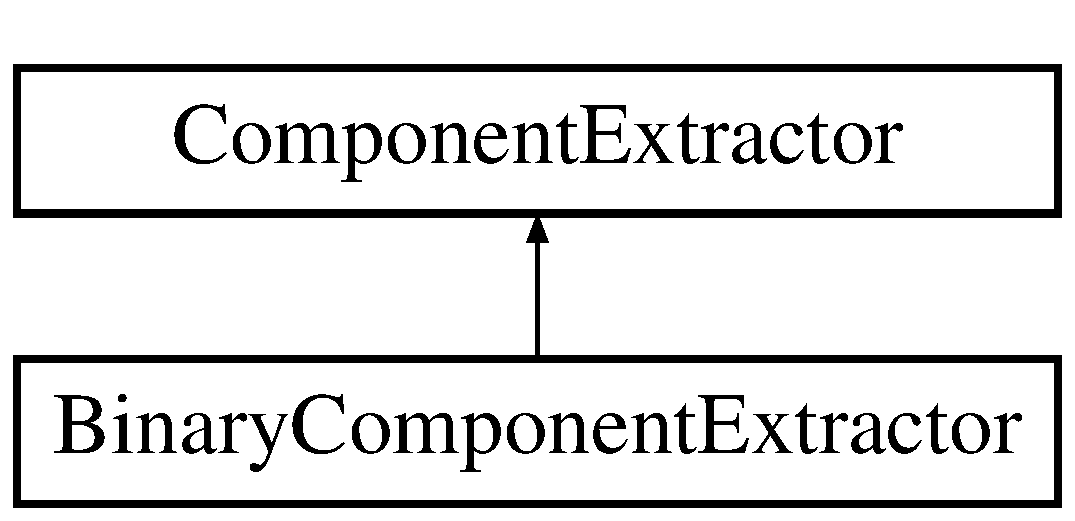
\includegraphics[height=2.000000cm]{class_component_extractor}
\end{center}
\end{figure}
\subsection*{Public Member Functions}
\begin{DoxyCompactItemize}
\item 
\hyperlink{class_component_extractor_adccc457807e0b48696f94d3c6d28e88f}{Component\+Extractor} (void)
\item 
\hyperlink{class_component_extractor_a4e079014da28395a14fb63babf10e1c6}{$\sim$\+Component\+Extractor} (void)
\item 
void \hyperlink{class_component_extractor_a3ef66896076dc20816fd656b8aeb1f96}{set\+Image} (\hyperlink{class_d_image}{D\+Image} $\ast$img)
\item 
virtual void \hyperlink{class_component_extractor_ac26bd7eec0e6caa7312f603bf2368d84}{extract} (vector$<$ \hyperlink{class_connected_component}{Connected\+Component} $\ast$ $>$ \&)=0
\end{DoxyCompactItemize}
\subsection*{Protected Attributes}
\begin{DoxyCompactItemize}
\item 
\hyperlink{class_d_image}{D\+Image} $\ast$ \hyperlink{class_component_extractor_a57494f356e871fc5216eb13fbdb76f0b}{\+\_\+image}
\end{DoxyCompactItemize}


\subsection{Constructor \& Destructor Documentation}
\hypertarget{class_component_extractor_adccc457807e0b48696f94d3c6d28e88f}{\index{Component\+Extractor@{Component\+Extractor}!Component\+Extractor@{Component\+Extractor}}
\index{Component\+Extractor@{Component\+Extractor}!Component\+Extractor@{Component\+Extractor}}
\subsubsection[{Component\+Extractor}]{\setlength{\rightskip}{0pt plus 5cm}Component\+Extractor\+::\+Component\+Extractor (
\begin{DoxyParamCaption}
\item[{void}]{}
\end{DoxyParamCaption}
)\hspace{0.3cm}{\ttfamily [inline]}}}\label{class_component_extractor_adccc457807e0b48696f94d3c6d28e88f}
\hypertarget{class_component_extractor_a4e079014da28395a14fb63babf10e1c6}{\index{Component\+Extractor@{Component\+Extractor}!````~Component\+Extractor@{$\sim$\+Component\+Extractor}}
\index{````~Component\+Extractor@{$\sim$\+Component\+Extractor}!Component\+Extractor@{Component\+Extractor}}
\subsubsection[{$\sim$\+Component\+Extractor}]{\setlength{\rightskip}{0pt plus 5cm}Component\+Extractor\+::$\sim$\+Component\+Extractor (
\begin{DoxyParamCaption}
\item[{void}]{}
\end{DoxyParamCaption}
)\hspace{0.3cm}{\ttfamily [inline]}}}\label{class_component_extractor_a4e079014da28395a14fb63babf10e1c6}


\subsection{Member Function Documentation}
\hypertarget{class_component_extractor_ac26bd7eec0e6caa7312f603bf2368d84}{\index{Component\+Extractor@{Component\+Extractor}!extract@{extract}}
\index{extract@{extract}!Component\+Extractor@{Component\+Extractor}}
\subsubsection[{extract}]{\setlength{\rightskip}{0pt plus 5cm}virtual void Component\+Extractor\+::extract (
\begin{DoxyParamCaption}
\item[{vector$<$ {\bf Connected\+Component} $\ast$ $>$ \&}]{}
\end{DoxyParamCaption}
)\hspace{0.3cm}{\ttfamily [pure virtual]}}}\label{class_component_extractor_ac26bd7eec0e6caa7312f603bf2368d84}


Implemented in \hyperlink{class_binary_component_extractor_a16232815f3a3e8e28fd80a733ff71383}{Binary\+Component\+Extractor}.

\hypertarget{class_component_extractor_a3ef66896076dc20816fd656b8aeb1f96}{\index{Component\+Extractor@{Component\+Extractor}!set\+Image@{set\+Image}}
\index{set\+Image@{set\+Image}!Component\+Extractor@{Component\+Extractor}}
\subsubsection[{set\+Image}]{\setlength{\rightskip}{0pt plus 5cm}void Component\+Extractor\+::set\+Image (
\begin{DoxyParamCaption}
\item[{{\bf D\+Image} $\ast$}]{img}
\end{DoxyParamCaption}
)\hspace{0.3cm}{\ttfamily [inline]}}}\label{class_component_extractor_a3ef66896076dc20816fd656b8aeb1f96}


\subsection{Member Data Documentation}
\hypertarget{class_component_extractor_a57494f356e871fc5216eb13fbdb76f0b}{\index{Component\+Extractor@{Component\+Extractor}!\+\_\+image@{\+\_\+image}}
\index{\+\_\+image@{\+\_\+image}!Component\+Extractor@{Component\+Extractor}}
\subsubsection[{\+\_\+image}]{\setlength{\rightskip}{0pt plus 5cm}{\bf D\+Image}$\ast$ Component\+Extractor\+::\+\_\+image\hspace{0.3cm}{\ttfamily [protected]}}}\label{class_component_extractor_a57494f356e871fc5216eb13fbdb76f0b}


The documentation for this class was generated from the following file\+:\begin{DoxyCompactItemize}
\item 
Manuscript\+App/\hyperlink{_component_extractor_8h}{Component\+Extractor.\+h}\end{DoxyCompactItemize}

\hypertarget{class_connected_component}{\section{Connected\+Component Class Reference}
\label{class_connected_component}\index{Connected\+Component@{Connected\+Component}}
}


Connected component.  




{\ttfamily \#include $<$Connected\+Component.\+h$>$}

\subsection*{Public Member Functions}
\begin{DoxyCompactItemize}
\item 
\hyperlink{class_connected_component_a80f5acb7e4c10b17ab1d9dd1e5bbe308}{Connected\+Component} (vector$<$ Point $>$ \&contour)
\begin{DoxyCompactList}\small\item\em Constructor. \end{DoxyCompactList}\item 
\hyperlink{class_connected_component_af69288c391283d9ca4d017d435c840c9}{Connected\+Component} (void)
\begin{DoxyCompactList}\small\item\em Default constructor. \end{DoxyCompactList}\item 
\hyperlink{class_connected_component_a91f368cd2b9c725ba1ef610c0d18e223}{$\sim$\+Connected\+Component} (void)
\item 
void \hyperlink{class_connected_component_ac13a32125f8c05e118dcaa1fd57eacfb}{set\+Image} (Mat img)
\item 
void \hyperlink{class_connected_component_abd451aa4596f6e4bfb2c4b74b1764789}{set\+Image} (Mat img, Rect \&rect)
\item 
Mat \hyperlink{class_connected_component_ad25f944f3627225427501c1a1cd7dc45}{get\+Image} ()
\item 
\hyperlink{class_contour}{Contour} \& \hyperlink{class_connected_component_ae2272acc6e94fc8e2fa7f87e4e17c944}{get\+Contour} ()
\item 
void \hyperlink{class_connected_component_a391767f0886946771bf138e3d136b192}{add\+Child} (\hyperlink{class_connected_component}{Connected\+Component} $\ast$component)
\begin{DoxyCompactList}\small\item\em Adds a child component. A child component is a component inside the current one \end{DoxyCompactList}\item 
Rect \hyperlink{class_connected_component_a7be353a1c50182b97b4f4e36d1bb5275}{get\+Bound\+Rect} ()
\item 
\hyperlink{class_connected_component}{Connected\+Component} $\ast$ \hyperlink{class_connected_component_a9ac344dd99b73e26ba9f12e632db9a81}{get\+Parent} ()
\item 
vector$<$ \hyperlink{class_connected_component}{Connected\+Component} $\ast$ $>$ \& \hyperlink{class_connected_component_a3d061e6cd4e5bf337b084a3463ea8bb0}{get\+Children} ()
\item 
int \hyperlink{class_connected_component_acca10d6015b6dbbf07fd111b07b5dee9}{border\+Type} (Mat mat, int row, int col, char mask, int \&trace)
\item 
void \hyperlink{class_connected_component_afbf7969c6c69fa5c603ca819d809c820}{set\+Parent} (\hyperlink{class_connected_component}{Connected\+Component} $\ast$parent)
\item 
void \hyperlink{class_connected_component_a9cbcbbd6f27b0d5981522da5aa63ddac}{fill\+Component\+On\+Mat} (Mat mat, char mask, char filler)
\item 
void \hyperlink{class_connected_component_acf50ca5ed3d677faaff0b160b1e2a136}{draw} (Mat img, Scalar clr, bool isclosed, int thickness, int line\+\_\+type)
\begin{DoxyCompactList}\small\item\em Draws. \end{DoxyCompactList}\end{DoxyCompactItemize}
\subsection*{Protected Attributes}
\begin{DoxyCompactItemize}
\item 
Mat \hyperlink{class_connected_component_aeffe49ad736a5be430f40ffe2816234b}{\+\_\+image}
\item 
\hyperlink{class_connected_component}{Connected\+Component} $\ast$ \hyperlink{class_connected_component_a802edcad018e25fbf4398d3c1eaad926}{\+\_\+parent}
\item 
\hyperlink{class_contour}{Contour} \hyperlink{class_connected_component_ac41ea811b504bd7b57ed2cfaf6a73e04}{\+\_\+contour}
\item 
String \hyperlink{class_connected_component_a3d7c59ca80f6304b1f07a0e196a45bc1}{\+\_\+string}
\item 
vector$<$ \hyperlink{class_connected_component}{Connected\+Component} $\ast$ $>$ \hyperlink{class_connected_component_a68dde04250c15d018d774d55b8dc521c}{\+\_\+children}
\end{DoxyCompactItemize}


\subsection{Detailed Description}
Connected component. 

El Sana, 2/9/2012. 

\subsection{Constructor \& Destructor Documentation}
\hypertarget{class_connected_component_a80f5acb7e4c10b17ab1d9dd1e5bbe308}{\index{Connected\+Component@{Connected\+Component}!Connected\+Component@{Connected\+Component}}
\index{Connected\+Component@{Connected\+Component}!Connected\+Component@{Connected\+Component}}
\subsubsection[{Connected\+Component}]{\setlength{\rightskip}{0pt plus 5cm}Connected\+Component\+::\+Connected\+Component (
\begin{DoxyParamCaption}
\item[{vector$<$ Point $>$ \&}]{contour}
\end{DoxyParamCaption}
)}}\label{class_connected_component_a80f5acb7e4c10b17ab1d9dd1e5bbe308}


Constructor. 

El Sana, 2/9/2012. 


\begin{DoxyParams}{Parameters}
{\em contour} & \mbox{[}in\mbox{]} The contour of the connected component. \\
\hline
\end{DoxyParams}
\hypertarget{class_connected_component_af69288c391283d9ca4d017d435c840c9}{\index{Connected\+Component@{Connected\+Component}!Connected\+Component@{Connected\+Component}}
\index{Connected\+Component@{Connected\+Component}!Connected\+Component@{Connected\+Component}}
\subsubsection[{Connected\+Component}]{\setlength{\rightskip}{0pt plus 5cm}Connected\+Component\+::\+Connected\+Component (
\begin{DoxyParamCaption}
\item[{void}]{}
\end{DoxyParamCaption}
)}}\label{class_connected_component_af69288c391283d9ca4d017d435c840c9}


Default constructor. 

El Sana, 2/9/2012. \hypertarget{class_connected_component_a91f368cd2b9c725ba1ef610c0d18e223}{\index{Connected\+Component@{Connected\+Component}!````~Connected\+Component@{$\sim$\+Connected\+Component}}
\index{````~Connected\+Component@{$\sim$\+Connected\+Component}!Connected\+Component@{Connected\+Component}}
\subsubsection[{$\sim$\+Connected\+Component}]{\setlength{\rightskip}{0pt plus 5cm}Connected\+Component\+::$\sim$\+Connected\+Component (
\begin{DoxyParamCaption}
\item[{void}]{}
\end{DoxyParamCaption}
)}}\label{class_connected_component_a91f368cd2b9c725ba1ef610c0d18e223}


\subsection{Member Function Documentation}
\hypertarget{class_connected_component_a391767f0886946771bf138e3d136b192}{\index{Connected\+Component@{Connected\+Component}!add\+Child@{add\+Child}}
\index{add\+Child@{add\+Child}!Connected\+Component@{Connected\+Component}}
\subsubsection[{add\+Child}]{\setlength{\rightskip}{0pt plus 5cm}void Connected\+Component\+::add\+Child (
\begin{DoxyParamCaption}
\item[{{\bf Connected\+Component} $\ast$}]{component}
\end{DoxyParamCaption}
)}}\label{class_connected_component_a391767f0886946771bf138e3d136b192}


Adds a child component. A child component is a component inside the current one 

El Sana, 2/9/2012. 


\begin{DoxyParams}{Parameters}
{\em component} & \mbox{[}in\mbox{]} the component. \\
\hline
\end{DoxyParams}
\hypertarget{class_connected_component_acca10d6015b6dbbf07fd111b07b5dee9}{\index{Connected\+Component@{Connected\+Component}!border\+Type@{border\+Type}}
\index{border\+Type@{border\+Type}!Connected\+Component@{Connected\+Component}}
\subsubsection[{border\+Type}]{\setlength{\rightskip}{0pt plus 5cm}int Connected\+Component\+::border\+Type (
\begin{DoxyParamCaption}
\item[{Mat}]{mat, }
\item[{int}]{row, }
\item[{int}]{col, }
\item[{char}]{mask, }
\item[{int \&}]{trace}
\end{DoxyParamCaption}
)}}\label{class_connected_component_acca10d6015b6dbbf07fd111b07b5dee9}
\hypertarget{class_connected_component_acf50ca5ed3d677faaff0b160b1e2a136}{\index{Connected\+Component@{Connected\+Component}!draw@{draw}}
\index{draw@{draw}!Connected\+Component@{Connected\+Component}}
\subsubsection[{draw}]{\setlength{\rightskip}{0pt plus 5cm}void Connected\+Component\+::draw (
\begin{DoxyParamCaption}
\item[{Mat}]{img, }
\item[{Scalar}]{clr, }
\item[{bool}]{isclosed, }
\item[{int}]{thickness, }
\item[{int}]{line\+\_\+type}
\end{DoxyParamCaption}
)}}\label{class_connected_component_acf50ca5ed3d677faaff0b160b1e2a136}


Draws. 

El Sana, 2/9/2012. 


\begin{DoxyParams}{Parameters}
{\em img} & The image. \\
\hline
{\em clr} & The colour. \\
\hline
{\em isclosed} & true if isclosed. \\
\hline
{\em thickness} & The thickness. \\
\hline
{\em line\+\_\+type} & Type of the line. \\
\hline
\end{DoxyParams}
\hypertarget{class_connected_component_a9cbcbbd6f27b0d5981522da5aa63ddac}{\index{Connected\+Component@{Connected\+Component}!fill\+Component\+On\+Mat@{fill\+Component\+On\+Mat}}
\index{fill\+Component\+On\+Mat@{fill\+Component\+On\+Mat}!Connected\+Component@{Connected\+Component}}
\subsubsection[{fill\+Component\+On\+Mat}]{\setlength{\rightskip}{0pt plus 5cm}void Connected\+Component\+::fill\+Component\+On\+Mat (
\begin{DoxyParamCaption}
\item[{Mat}]{mat, }
\item[{char}]{mask, }
\item[{char}]{filler}
\end{DoxyParamCaption}
)}}\label{class_connected_component_a9cbcbbd6f27b0d5981522da5aa63ddac}
\hypertarget{class_connected_component_a7be353a1c50182b97b4f4e36d1bb5275}{\index{Connected\+Component@{Connected\+Component}!get\+Bound\+Rect@{get\+Bound\+Rect}}
\index{get\+Bound\+Rect@{get\+Bound\+Rect}!Connected\+Component@{Connected\+Component}}
\subsubsection[{get\+Bound\+Rect}]{\setlength{\rightskip}{0pt plus 5cm}Rect Connected\+Component\+::get\+Bound\+Rect (
\begin{DoxyParamCaption}
{}
\end{DoxyParamCaption}
)\hspace{0.3cm}{\ttfamily [inline]}}}\label{class_connected_component_a7be353a1c50182b97b4f4e36d1bb5275}
\hypertarget{class_connected_component_a3d061e6cd4e5bf337b084a3463ea8bb0}{\index{Connected\+Component@{Connected\+Component}!get\+Children@{get\+Children}}
\index{get\+Children@{get\+Children}!Connected\+Component@{Connected\+Component}}
\subsubsection[{get\+Children}]{\setlength{\rightskip}{0pt plus 5cm}vector$<${\bf Connected\+Component}$\ast$$>$\& Connected\+Component\+::get\+Children (
\begin{DoxyParamCaption}
{}
\end{DoxyParamCaption}
)\hspace{0.3cm}{\ttfamily [inline]}}}\label{class_connected_component_a3d061e6cd4e5bf337b084a3463ea8bb0}
\hypertarget{class_connected_component_ae2272acc6e94fc8e2fa7f87e4e17c944}{\index{Connected\+Component@{Connected\+Component}!get\+Contour@{get\+Contour}}
\index{get\+Contour@{get\+Contour}!Connected\+Component@{Connected\+Component}}
\subsubsection[{get\+Contour}]{\setlength{\rightskip}{0pt plus 5cm}{\bf Contour}\& Connected\+Component\+::get\+Contour (
\begin{DoxyParamCaption}
{}
\end{DoxyParamCaption}
)\hspace{0.3cm}{\ttfamily [inline]}}}\label{class_connected_component_ae2272acc6e94fc8e2fa7f87e4e17c944}
\hypertarget{class_connected_component_ad25f944f3627225427501c1a1cd7dc45}{\index{Connected\+Component@{Connected\+Component}!get\+Image@{get\+Image}}
\index{get\+Image@{get\+Image}!Connected\+Component@{Connected\+Component}}
\subsubsection[{get\+Image}]{\setlength{\rightskip}{0pt plus 5cm}Mat Connected\+Component\+::get\+Image (
\begin{DoxyParamCaption}
{}
\end{DoxyParamCaption}
)\hspace{0.3cm}{\ttfamily [inline]}}}\label{class_connected_component_ad25f944f3627225427501c1a1cd7dc45}
\hypertarget{class_connected_component_a9ac344dd99b73e26ba9f12e632db9a81}{\index{Connected\+Component@{Connected\+Component}!get\+Parent@{get\+Parent}}
\index{get\+Parent@{get\+Parent}!Connected\+Component@{Connected\+Component}}
\subsubsection[{get\+Parent}]{\setlength{\rightskip}{0pt plus 5cm}{\bf Connected\+Component}$\ast$ Connected\+Component\+::get\+Parent (
\begin{DoxyParamCaption}
{}
\end{DoxyParamCaption}
)\hspace{0.3cm}{\ttfamily [inline]}}}\label{class_connected_component_a9ac344dd99b73e26ba9f12e632db9a81}
\hypertarget{class_connected_component_ac13a32125f8c05e118dcaa1fd57eacfb}{\index{Connected\+Component@{Connected\+Component}!set\+Image@{set\+Image}}
\index{set\+Image@{set\+Image}!Connected\+Component@{Connected\+Component}}
\subsubsection[{set\+Image}]{\setlength{\rightskip}{0pt plus 5cm}void Connected\+Component\+::set\+Image (
\begin{DoxyParamCaption}
\item[{Mat}]{img}
\end{DoxyParamCaption}
)\hspace{0.3cm}{\ttfamily [inline]}}}\label{class_connected_component_ac13a32125f8c05e118dcaa1fd57eacfb}
\hypertarget{class_connected_component_abd451aa4596f6e4bfb2c4b74b1764789}{\index{Connected\+Component@{Connected\+Component}!set\+Image@{set\+Image}}
\index{set\+Image@{set\+Image}!Connected\+Component@{Connected\+Component}}
\subsubsection[{set\+Image}]{\setlength{\rightskip}{0pt plus 5cm}void Connected\+Component\+::set\+Image (
\begin{DoxyParamCaption}
\item[{Mat}]{img, }
\item[{Rect \&}]{rect}
\end{DoxyParamCaption}
)\hspace{0.3cm}{\ttfamily [inline]}}}\label{class_connected_component_abd451aa4596f6e4bfb2c4b74b1764789}
\hypertarget{class_connected_component_afbf7969c6c69fa5c603ca819d809c820}{\index{Connected\+Component@{Connected\+Component}!set\+Parent@{set\+Parent}}
\index{set\+Parent@{set\+Parent}!Connected\+Component@{Connected\+Component}}
\subsubsection[{set\+Parent}]{\setlength{\rightskip}{0pt plus 5cm}void Connected\+Component\+::set\+Parent (
\begin{DoxyParamCaption}
\item[{{\bf Connected\+Component} $\ast$}]{parent}
\end{DoxyParamCaption}
)\hspace{0.3cm}{\ttfamily [inline]}}}\label{class_connected_component_afbf7969c6c69fa5c603ca819d809c820}


\subsection{Member Data Documentation}
\hypertarget{class_connected_component_a68dde04250c15d018d774d55b8dc521c}{\index{Connected\+Component@{Connected\+Component}!\+\_\+children@{\+\_\+children}}
\index{\+\_\+children@{\+\_\+children}!Connected\+Component@{Connected\+Component}}
\subsubsection[{\+\_\+children}]{\setlength{\rightskip}{0pt plus 5cm}vector$<${\bf Connected\+Component}$\ast$$>$ Connected\+Component\+::\+\_\+children\hspace{0.3cm}{\ttfamily [protected]}}}\label{class_connected_component_a68dde04250c15d018d774d55b8dc521c}
\hypertarget{class_connected_component_ac41ea811b504bd7b57ed2cfaf6a73e04}{\index{Connected\+Component@{Connected\+Component}!\+\_\+contour@{\+\_\+contour}}
\index{\+\_\+contour@{\+\_\+contour}!Connected\+Component@{Connected\+Component}}
\subsubsection[{\+\_\+contour}]{\setlength{\rightskip}{0pt plus 5cm}{\bf Contour} Connected\+Component\+::\+\_\+contour\hspace{0.3cm}{\ttfamily [protected]}}}\label{class_connected_component_ac41ea811b504bd7b57ed2cfaf6a73e04}
\hypertarget{class_connected_component_aeffe49ad736a5be430f40ffe2816234b}{\index{Connected\+Component@{Connected\+Component}!\+\_\+image@{\+\_\+image}}
\index{\+\_\+image@{\+\_\+image}!Connected\+Component@{Connected\+Component}}
\subsubsection[{\+\_\+image}]{\setlength{\rightskip}{0pt plus 5cm}Mat Connected\+Component\+::\+\_\+image\hspace{0.3cm}{\ttfamily [protected]}}}\label{class_connected_component_aeffe49ad736a5be430f40ffe2816234b}
\hypertarget{class_connected_component_a802edcad018e25fbf4398d3c1eaad926}{\index{Connected\+Component@{Connected\+Component}!\+\_\+parent@{\+\_\+parent}}
\index{\+\_\+parent@{\+\_\+parent}!Connected\+Component@{Connected\+Component}}
\subsubsection[{\+\_\+parent}]{\setlength{\rightskip}{0pt plus 5cm}{\bf Connected\+Component}$\ast$ Connected\+Component\+::\+\_\+parent\hspace{0.3cm}{\ttfamily [protected]}}}\label{class_connected_component_a802edcad018e25fbf4398d3c1eaad926}
\hypertarget{class_connected_component_a3d7c59ca80f6304b1f07a0e196a45bc1}{\index{Connected\+Component@{Connected\+Component}!\+\_\+string@{\+\_\+string}}
\index{\+\_\+string@{\+\_\+string}!Connected\+Component@{Connected\+Component}}
\subsubsection[{\+\_\+string}]{\setlength{\rightskip}{0pt plus 5cm}String Connected\+Component\+::\+\_\+string\hspace{0.3cm}{\ttfamily [protected]}}}\label{class_connected_component_a3d7c59ca80f6304b1f07a0e196a45bc1}


The documentation for this class was generated from the following files\+:\begin{DoxyCompactItemize}
\item 
Manuscript\+App/\hyperlink{_connected_component_8h}{Connected\+Component.\+h}\item 
Manuscript\+App/\hyperlink{_connected_component_8cpp}{Connected\+Component.\+cpp}\end{DoxyCompactItemize}

\hypertarget{class_contour}{\section{Contour Class Reference}
\label{class_contour}\index{Contour@{Contour}}
}


{\ttfamily \#include $<$Contour.\+h$>$}

\subsection*{Public Member Functions}
\begin{DoxyCompactItemize}
\item 
\hyperlink{class_contour_ac31a122f91e1a4a2462ecb802ed7170f}{Contour} (void)
\item 
\hyperlink{class_contour_ae8f5b046ccf380b396f54de0d01e731f}{$\sim$\+Contour} (void)
\item 
vector$<$ cv\+::\+Point $>$ \& \hyperlink{class_contour_abc363aff3d9b7642daa6cf3496b7bea0}{get\+Points} ()
\item 
Rect \& \hyperlink{class_contour_a6a0a7792ef282071a7bbde523ec0e96d}{get\+Bound\+Rect} ()
\item 
\hyperlink{_contour_8h_a25057779f97dd06805ea5fcf36635c40}{Orientation} \hyperlink{class_contour_a16c54703d99650fcca6752da59deaab7}{get\+Orientation} ()
\item 
void \hyperlink{class_contour_a866591bd98e4ebdbd511eb43ef511fd3}{set\+Center} ()
\item 
Point \hyperlink{class_contour_a7efb5a9005069c53af5fd291dc17d902}{get\+Center} ()
\item 
void \hyperlink{class_contour_a2064d4cd92143ab0e466ecba4eeb3b75}{set\+Points} (vector$<$ cv\+::\+Point $>$ p)
\item 
Mat \hyperlink{class_contour_af6da2b9bb1d742b35fb9c2c11f7b1dbe}{get\+Mat} (vector$<$ Point $>$ \&pts)
\item 
void \hyperlink{class_contour_ac3b85c445a9a648ebec59fdd2413194d}{set\+Bound\+Rect} ()
\begin{DoxyCompactList}\small\item\em Sets the bounding rectangle of the contour, using its points. \end{DoxyCompactList}\item 
void \hyperlink{class_contour_ad07917ec771f6c5df764fdeac7841613}{set\+Orientation} ()
\item 
float \hyperlink{class_contour_a29fab9bc4b308e3230172bda77650a72}{get\+Importance} (int i)
\begin{DoxyCompactList}\small\item\em Gets an importance, which is computed as the size of the thriangle defined by the vertex and its two adjacent neighbors \end{DoxyCompactList}\item 
int \hyperlink{class_contour_a89afece7e3b513654cee39410ed57e86}{get\+Least\+Important} ()
\begin{DoxyCompactList}\small\item\em Return the vertex with the least importance value \end{DoxyCompactList}\item 
void \hyperlink{class_contour_a1d45bb2a1ca97b4fa9418f9c43318f2a}{remove\+Vertex} (int i)
\begin{DoxyCompactList}\small\item\em Removes the vertex i from the contour (boundary). \end{DoxyCompactList}\item 
int \hyperlink{class_contour_a3f30ccff7776c7aacae37145df5da467}{remove\+Least\+Important} ()
\begin{DoxyCompactList}\small\item\em Removes the vertex with least importance value \end{DoxyCompactList}\item 
void \hyperlink{class_contour_ac36273da0f11bf3095087f26ca3c6440}{draw\+On\+Image} (Mat mat, char filler)
\item 
float \hyperlink{class_contour_a6c162802a4123888526f43561e7584f5}{get\+Area} ()
\begin{DoxyCompactList}\small\item\em Gets the area of a contour, the area is computed each time it is called, i.\+e., it is not stored \end{DoxyCompactList}\end{DoxyCompactItemize}
\subsection*{Protected Attributes}
\begin{DoxyCompactItemize}
\item 
vector$<$ cv\+::\+Point $>$ \hyperlink{class_contour_a5fe5723655cd3e3a1e40a433565ed9f7}{\+\_\+points}
\item 
Rect \hyperlink{class_contour_aefe73b0c7479e0a6bca7c76e5cc4aa6d}{\+\_\+brect}
\item 
Point2f \hyperlink{class_contour_a60351d0013e44e0ea12b8c2f227b2d74}{\+\_\+center}
\item 
\hyperlink{_contour_8h_a25057779f97dd06805ea5fcf36635c40}{Orientation} \hyperlink{class_contour_a946768dfb1a6b340165360db2bf279db}{\+\_\+orientation}
\item 
vector$<$ \hyperlink{_contour_8h_a8f46426628d6edd9ed397144417e79ee}{Vertex\+Weight} $>$ \hyperlink{class_contour_a7a26f7919fa25f04975ab3949152437b}{\+\_\+heap}
\end{DoxyCompactItemize}


\subsection{Constructor \& Destructor Documentation}
\hypertarget{class_contour_ac31a122f91e1a4a2462ecb802ed7170f}{\index{Contour@{Contour}!Contour@{Contour}}
\index{Contour@{Contour}!Contour@{Contour}}
\subsubsection[{Contour}]{\setlength{\rightskip}{0pt plus 5cm}Contour\+::\+Contour (
\begin{DoxyParamCaption}
\item[{void}]{}
\end{DoxyParamCaption}
)\hspace{0.3cm}{\ttfamily [inline]}}}\label{class_contour_ac31a122f91e1a4a2462ecb802ed7170f}
\hypertarget{class_contour_ae8f5b046ccf380b396f54de0d01e731f}{\index{Contour@{Contour}!````~Contour@{$\sim$\+Contour}}
\index{````~Contour@{$\sim$\+Contour}!Contour@{Contour}}
\subsubsection[{$\sim$\+Contour}]{\setlength{\rightskip}{0pt plus 5cm}Contour\+::$\sim$\+Contour (
\begin{DoxyParamCaption}
\item[{void}]{}
\end{DoxyParamCaption}
)\hspace{0.3cm}{\ttfamily [inline]}}}\label{class_contour_ae8f5b046ccf380b396f54de0d01e731f}


\subsection{Member Function Documentation}
\hypertarget{class_contour_ac36273da0f11bf3095087f26ca3c6440}{\index{Contour@{Contour}!draw\+On\+Image@{draw\+On\+Image}}
\index{draw\+On\+Image@{draw\+On\+Image}!Contour@{Contour}}
\subsubsection[{draw\+On\+Image}]{\setlength{\rightskip}{0pt plus 5cm}void Contour\+::draw\+On\+Image (
\begin{DoxyParamCaption}
\item[{Mat}]{mat, }
\item[{char}]{filler}
\end{DoxyParamCaption}
)}}\label{class_contour_ac36273da0f11bf3095087f26ca3c6440}
\hypertarget{class_contour_a6c162802a4123888526f43561e7584f5}{\index{Contour@{Contour}!get\+Area@{get\+Area}}
\index{get\+Area@{get\+Area}!Contour@{Contour}}
\subsubsection[{get\+Area}]{\setlength{\rightskip}{0pt plus 5cm}float Contour\+::get\+Area (
\begin{DoxyParamCaption}
{}
\end{DoxyParamCaption}
)}}\label{class_contour_a6c162802a4123888526f43561e7584f5}


Gets the area of a contour, the area is computed each time it is called, i.\+e., it is not stored 

El Sana, 2/15/2012. 

\begin{DoxyReturn}{Returns}
The area. 
\end{DoxyReturn}
\hypertarget{class_contour_a6a0a7792ef282071a7bbde523ec0e96d}{\index{Contour@{Contour}!get\+Bound\+Rect@{get\+Bound\+Rect}}
\index{get\+Bound\+Rect@{get\+Bound\+Rect}!Contour@{Contour}}
\subsubsection[{get\+Bound\+Rect}]{\setlength{\rightskip}{0pt plus 5cm}Rect\& Contour\+::get\+Bound\+Rect (
\begin{DoxyParamCaption}
{}
\end{DoxyParamCaption}
)\hspace{0.3cm}{\ttfamily [inline]}}}\label{class_contour_a6a0a7792ef282071a7bbde523ec0e96d}
\hypertarget{class_contour_a7efb5a9005069c53af5fd291dc17d902}{\index{Contour@{Contour}!get\+Center@{get\+Center}}
\index{get\+Center@{get\+Center}!Contour@{Contour}}
\subsubsection[{get\+Center}]{\setlength{\rightskip}{0pt plus 5cm}Point Contour\+::get\+Center (
\begin{DoxyParamCaption}
{}
\end{DoxyParamCaption}
)\hspace{0.3cm}{\ttfamily [inline]}}}\label{class_contour_a7efb5a9005069c53af5fd291dc17d902}
\hypertarget{class_contour_a29fab9bc4b308e3230172bda77650a72}{\index{Contour@{Contour}!get\+Importance@{get\+Importance}}
\index{get\+Importance@{get\+Importance}!Contour@{Contour}}
\subsubsection[{get\+Importance}]{\setlength{\rightskip}{0pt plus 5cm}float Contour\+::get\+Importance (
\begin{DoxyParamCaption}
\item[{int}]{i}
\end{DoxyParamCaption}
)}}\label{class_contour_a29fab9bc4b308e3230172bda77650a72}


Gets an importance, which is computed as the size of the thriangle defined by the vertex and its two adjacent neighbors 

El Sana, 2/15/2012. 


\begin{DoxyParams}{Parameters}
{\em i} & Zero-\/based index of the. \\
\hline
\end{DoxyParams}


\begin{DoxyReturn}{Returns}
The importance. 
\end{DoxyReturn}
\hypertarget{class_contour_a89afece7e3b513654cee39410ed57e86}{\index{Contour@{Contour}!get\+Least\+Important@{get\+Least\+Important}}
\index{get\+Least\+Important@{get\+Least\+Important}!Contour@{Contour}}
\subsubsection[{get\+Least\+Important}]{\setlength{\rightskip}{0pt plus 5cm}int Contour\+::get\+Least\+Important (
\begin{DoxyParamCaption}
{}
\end{DoxyParamCaption}
)}}\label{class_contour_a89afece7e3b513654cee39410ed57e86}


Return the vertex with the least importance value 

El Sana, 2/15/2012. 

\begin{DoxyReturn}{Returns}
The least important. 
\end{DoxyReturn}
\hypertarget{class_contour_af6da2b9bb1d742b35fb9c2c11f7b1dbe}{\index{Contour@{Contour}!get\+Mat@{get\+Mat}}
\index{get\+Mat@{get\+Mat}!Contour@{Contour}}
\subsubsection[{get\+Mat}]{\setlength{\rightskip}{0pt plus 5cm}Mat Contour\+::get\+Mat (
\begin{DoxyParamCaption}
\item[{vector$<$ Point $>$ \&}]{pts}
\end{DoxyParamCaption}
)}}\label{class_contour_af6da2b9bb1d742b35fb9c2c11f7b1dbe}
\hypertarget{class_contour_a16c54703d99650fcca6752da59deaab7}{\index{Contour@{Contour}!get\+Orientation@{get\+Orientation}}
\index{get\+Orientation@{get\+Orientation}!Contour@{Contour}}
\subsubsection[{get\+Orientation}]{\setlength{\rightskip}{0pt plus 5cm}{\bf Orientation} Contour\+::get\+Orientation (
\begin{DoxyParamCaption}
{}
\end{DoxyParamCaption}
)\hspace{0.3cm}{\ttfamily [inline]}}}\label{class_contour_a16c54703d99650fcca6752da59deaab7}
\hypertarget{class_contour_abc363aff3d9b7642daa6cf3496b7bea0}{\index{Contour@{Contour}!get\+Points@{get\+Points}}
\index{get\+Points@{get\+Points}!Contour@{Contour}}
\subsubsection[{get\+Points}]{\setlength{\rightskip}{0pt plus 5cm}vector$<$cv\+::\+Point$>$\& Contour\+::get\+Points (
\begin{DoxyParamCaption}
{}
\end{DoxyParamCaption}
)\hspace{0.3cm}{\ttfamily [inline]}}}\label{class_contour_abc363aff3d9b7642daa6cf3496b7bea0}
\hypertarget{class_contour_a3f30ccff7776c7aacae37145df5da467}{\index{Contour@{Contour}!remove\+Least\+Important@{remove\+Least\+Important}}
\index{remove\+Least\+Important@{remove\+Least\+Important}!Contour@{Contour}}
\subsubsection[{remove\+Least\+Important}]{\setlength{\rightskip}{0pt plus 5cm}int Contour\+::remove\+Least\+Important (
\begin{DoxyParamCaption}
{}
\end{DoxyParamCaption}
)}}\label{class_contour_a3f30ccff7776c7aacae37145df5da467}


Removes the vertex with least importance value 

El Sana, 2/15/2012. 

\begin{DoxyReturn}{Returns}
. 
\end{DoxyReturn}
\hypertarget{class_contour_a1d45bb2a1ca97b4fa9418f9c43318f2a}{\index{Contour@{Contour}!remove\+Vertex@{remove\+Vertex}}
\index{remove\+Vertex@{remove\+Vertex}!Contour@{Contour}}
\subsubsection[{remove\+Vertex}]{\setlength{\rightskip}{0pt plus 5cm}void Contour\+::remove\+Vertex (
\begin{DoxyParamCaption}
\item[{int}]{i}
\end{DoxyParamCaption}
)}}\label{class_contour_a1d45bb2a1ca97b4fa9418f9c43318f2a}


Removes the vertex i from the contour (boundary). 

El Sana, 2/15/2012. 


\begin{DoxyParams}{Parameters}
{\em i} & Zero-\/based index of the. \\
\hline
\end{DoxyParams}
\hypertarget{class_contour_ac3b85c445a9a648ebec59fdd2413194d}{\index{Contour@{Contour}!set\+Bound\+Rect@{set\+Bound\+Rect}}
\index{set\+Bound\+Rect@{set\+Bound\+Rect}!Contour@{Contour}}
\subsubsection[{set\+Bound\+Rect}]{\setlength{\rightskip}{0pt plus 5cm}void Contour\+::set\+Bound\+Rect (
\begin{DoxyParamCaption}
{}
\end{DoxyParamCaption}
)}}\label{class_contour_ac3b85c445a9a648ebec59fdd2413194d}


Sets the bounding rectangle of the contour, using its points. 

El Sana, 2/15/2012. \hypertarget{class_contour_a866591bd98e4ebdbd511eb43ef511fd3}{\index{Contour@{Contour}!set\+Center@{set\+Center}}
\index{set\+Center@{set\+Center}!Contour@{Contour}}
\subsubsection[{set\+Center}]{\setlength{\rightskip}{0pt plus 5cm}void Contour\+::set\+Center (
\begin{DoxyParamCaption}
{}
\end{DoxyParamCaption}
)}}\label{class_contour_a866591bd98e4ebdbd511eb43ef511fd3}
\hypertarget{class_contour_ad07917ec771f6c5df764fdeac7841613}{\index{Contour@{Contour}!set\+Orientation@{set\+Orientation}}
\index{set\+Orientation@{set\+Orientation}!Contour@{Contour}}
\subsubsection[{set\+Orientation}]{\setlength{\rightskip}{0pt plus 5cm}void Contour\+::set\+Orientation (
\begin{DoxyParamCaption}
{}
\end{DoxyParamCaption}
)}}\label{class_contour_ad07917ec771f6c5df764fdeac7841613}
\hypertarget{class_contour_a2064d4cd92143ab0e466ecba4eeb3b75}{\index{Contour@{Contour}!set\+Points@{set\+Points}}
\index{set\+Points@{set\+Points}!Contour@{Contour}}
\subsubsection[{set\+Points}]{\setlength{\rightskip}{0pt plus 5cm}void Contour\+::set\+Points (
\begin{DoxyParamCaption}
\item[{vector$<$ cv\+::\+Point $>$}]{p}
\end{DoxyParamCaption}
)\hspace{0.3cm}{\ttfamily [inline]}}}\label{class_contour_a2064d4cd92143ab0e466ecba4eeb3b75}


\subsection{Member Data Documentation}
\hypertarget{class_contour_aefe73b0c7479e0a6bca7c76e5cc4aa6d}{\index{Contour@{Contour}!\+\_\+brect@{\+\_\+brect}}
\index{\+\_\+brect@{\+\_\+brect}!Contour@{Contour}}
\subsubsection[{\+\_\+brect}]{\setlength{\rightskip}{0pt plus 5cm}Rect Contour\+::\+\_\+brect\hspace{0.3cm}{\ttfamily [protected]}}}\label{class_contour_aefe73b0c7479e0a6bca7c76e5cc4aa6d}
\hypertarget{class_contour_a60351d0013e44e0ea12b8c2f227b2d74}{\index{Contour@{Contour}!\+\_\+center@{\+\_\+center}}
\index{\+\_\+center@{\+\_\+center}!Contour@{Contour}}
\subsubsection[{\+\_\+center}]{\setlength{\rightskip}{0pt plus 5cm}Point2f Contour\+::\+\_\+center\hspace{0.3cm}{\ttfamily [protected]}}}\label{class_contour_a60351d0013e44e0ea12b8c2f227b2d74}
\hypertarget{class_contour_a7a26f7919fa25f04975ab3949152437b}{\index{Contour@{Contour}!\+\_\+heap@{\+\_\+heap}}
\index{\+\_\+heap@{\+\_\+heap}!Contour@{Contour}}
\subsubsection[{\+\_\+heap}]{\setlength{\rightskip}{0pt plus 5cm}vector$<${\bf Vertex\+Weight}$>$ Contour\+::\+\_\+heap\hspace{0.3cm}{\ttfamily [protected]}}}\label{class_contour_a7a26f7919fa25f04975ab3949152437b}
\hypertarget{class_contour_a946768dfb1a6b340165360db2bf279db}{\index{Contour@{Contour}!\+\_\+orientation@{\+\_\+orientation}}
\index{\+\_\+orientation@{\+\_\+orientation}!Contour@{Contour}}
\subsubsection[{\+\_\+orientation}]{\setlength{\rightskip}{0pt plus 5cm}{\bf Orientation} Contour\+::\+\_\+orientation\hspace{0.3cm}{\ttfamily [protected]}}}\label{class_contour_a946768dfb1a6b340165360db2bf279db}
\hypertarget{class_contour_a5fe5723655cd3e3a1e40a433565ed9f7}{\index{Contour@{Contour}!\+\_\+points@{\+\_\+points}}
\index{\+\_\+points@{\+\_\+points}!Contour@{Contour}}
\subsubsection[{\+\_\+points}]{\setlength{\rightskip}{0pt plus 5cm}vector$<$cv\+::\+Point$>$ Contour\+::\+\_\+points\hspace{0.3cm}{\ttfamily [protected]}}}\label{class_contour_a5fe5723655cd3e3a1e40a433565ed9f7}


The documentation for this class was generated from the following files\+:\begin{DoxyCompactItemize}
\item 
Manuscript\+App/\hyperlink{_contour_8h}{Contour.\+h}\item 
Manuscript\+App/\hyperlink{_contour_8cpp}{Contour.\+cpp}\end{DoxyCompactItemize}

\hypertarget{class_d_image}{\section{D\+Image Class Reference}
\label{class_d_image}\index{D\+Image@{D\+Image}}
}


{\ttfamily \#include $<$D\+Image.\+h$>$}

Inheritance diagram for D\+Image\+:\begin{figure}[H]
\begin{center}
\leavevmode
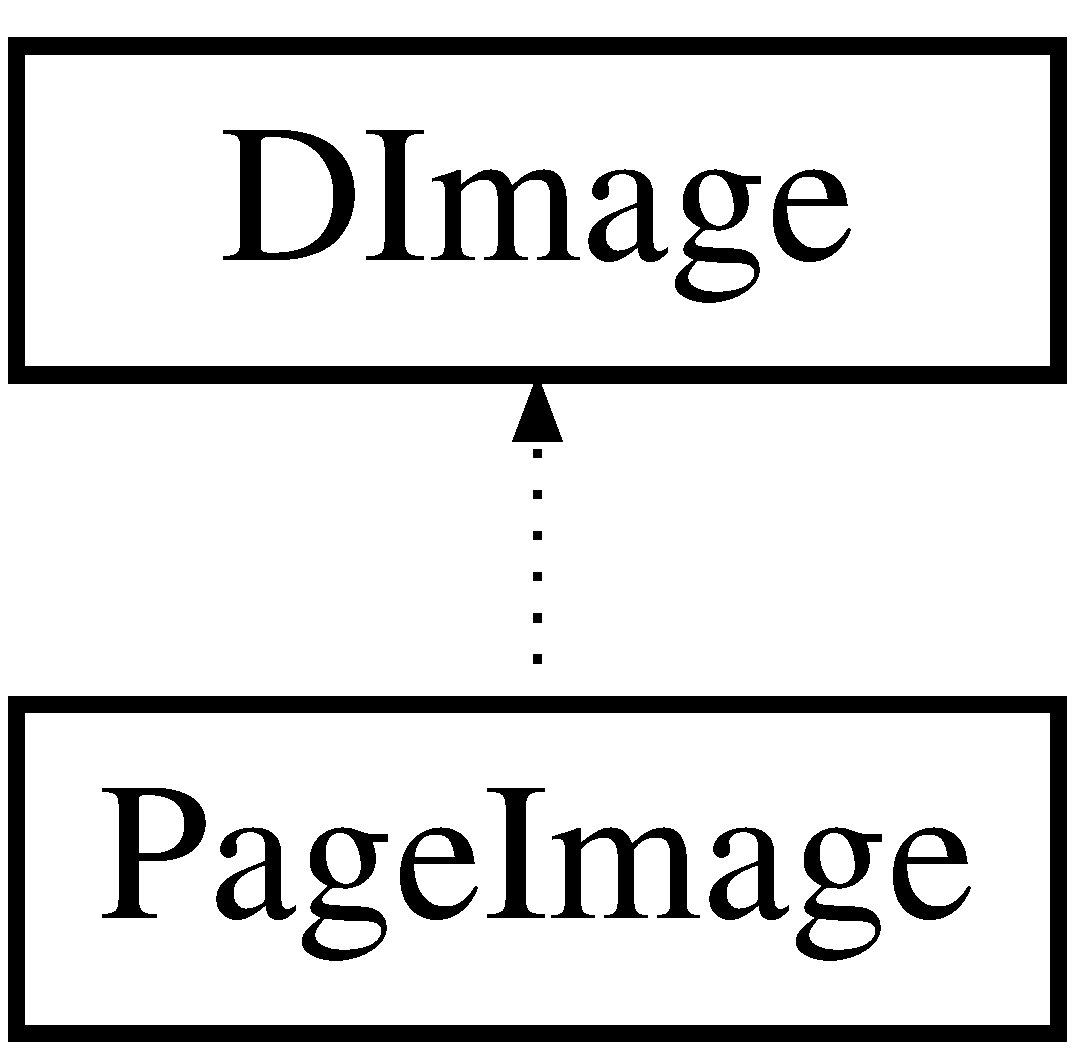
\includegraphics[height=2.000000cm]{class_d_image}
\end{center}
\end{figure}
\subsection*{Public Member Functions}
\begin{DoxyCompactItemize}
\item 
\hyperlink{class_d_image_ab276c7e2458e697fbff3366a27f9bf93}{D\+Image} ()
\item 
\hyperlink{class_d_image_a7d7c1b9cf26cf48c81b9d5cd424ab788}{D\+Image} (Mat mat)
\item 
\hyperlink{class_d_image_aa86a9aa92905deb0d8aab5f1298c6b9b}{$\sim$\+D\+Image} (void)
\item 
void \hyperlink{class_d_image_a4c4ee0a9910a21d200a469f945060fbe}{set\+Type} (int itype)
\item 
void \hyperlink{class_d_image_a7673f3ca0b1703a3401e7a953e7464e2}{set\+Format} (int iformat)
\item 
int \hyperlink{class_d_image_a80065ac2ff9eb49a68adde1f24494087}{get\+Format} ()
\item 
int \hyperlink{class_d_image_aad98497ac69ada8d00e14d1aadf11406}{get\+Type} ()
\item 
void \hyperlink{class_d_image_af7605a6d9d5bd6ca117507bd9fd00c2b}{set\+Mat} (Mat mat)
\item 
Mat \& \hyperlink{class_d_image_a1f875d1a50eff52cbd1ca119f5293c8d}{get\+Mat} ()
\item 
Point2f \hyperlink{class_d_image_a8127b81bd1bcafa719c8c39f868a61e8}{set\+C\+O\+M} ()
\item 
Point2f \hyperlink{class_d_image_a391b874fbd441d759a68582c5a1c65ff}{get\+C\+O\+M} ()
\item 
\hyperlink{class_d_image}{D\+Image} $\ast$ \hyperlink{class_d_image_af91df7fb4ff6ee2ff5d040bd5ae4356c}{convert} (int to\+\_\+type)
\item 
\hyperlink{class_d_image}{D\+Image} $\ast$ \hyperlink{class_d_image_abbd42491c1788bab34a871e5674e0ad4}{convert} (\hyperlink{class_image_converter}{Image\+Converter} \&ic)
\item 
\hyperlink{class_d_image}{D\+Image} $\ast$ \hyperlink{class_d_image_a62f8f2c9cd22264f31c94f352c2fb620}{enhance} (\hyperlink{class_image_enhancer}{Image\+Enhancer} \&ih)
\item 
\hyperlink{class_d_image}{D\+Image} $\ast$ \hyperlink{class_d_image_a30853028d3eee069389660a20178e57c}{project} (\hyperlink{class_image_projector}{Image\+Projector} \&ip)
\item 
\hyperlink{class_d_image}{D\+Image} $\ast$ \hyperlink{class_d_image_aabf5c54bbdfdfb7cde2aca18452d5ef1}{binarize} (\hyperlink{class_image_binarizer}{Image\+Binarizer} \&ib)
\item 
\hyperlink{class_d_image}{D\+Image} $\ast$ \hyperlink{class_d_image_ae3bb096400bf85dc02ee93578696471b}{filter} (\hyperlink{class_image_filter}{Image\+Filter} \&io)
\item 
void \hyperlink{class_d_image_a644022c2f892f2087e2345faf9219930}{extract\+Features} (\hyperlink{class_feature_extractor}{Feature\+Extractor} \&feature\+\_\+extractor, vector$<$ \hyperlink{class_feature}{Feature} $\ast$ $>$ \&feature\+\_\+list)
\item 
void \hyperlink{class_d_image_a4a60efb2e91c9a07a4d8f37b9bc4d086}{extract\+Components} (\hyperlink{class_component_extractor}{Component\+Extractor} \&ex, vector$<$ \hyperlink{class_connected_component}{Connected\+Component} $\ast$ $>$ \&v)
\item 
void \hyperlink{class_d_image_a56a11350bd9375dfe95a62abc2f4f8f8}{display} (String win)
\end{DoxyCompactItemize}
\subsection*{Static Public Attributes}
\begin{DoxyCompactItemize}
\item 
static const int \hyperlink{class_d_image_a5329679c0199806b9951d0442ec292f5}{D\+I\+F\+O\+R\+M\+A\+T\+\_\+\+U\+N\+S\+E\+T} = 0
\item 
static const int \hyperlink{class_d_image_a16e31de8a97ada87e8a077f72ff297d1}{D\+I\+F\+O\+R\+M\+A\+T\+\_\+\+R\+G\+B} = 1
\item 
static const int \hyperlink{class_d_image_ac2aef108a618db6d3e04924510ba9f35}{D\+I\+F\+O\+R\+M\+A\+T\+\_\+\+G\+R\+A\+Y} = 2
\item 
static const int \hyperlink{class_d_image_adf32af60452b52eb59922c9bb5f87119}{D\+I\+F\+O\+R\+M\+A\+T\+\_\+\+B\+I\+N\+A\+R\+Y} = 3
\item 
static const int \hyperlink{class_d_image_abf8ff1b3f61e5a15641bc672eaa9922e}{D\+I\+T\+Y\+P\+E\+\_\+\+U\+N\+S\+E\+T} = 0
\item 
static const int \hyperlink{class_d_image_a6a2aac0adab6d13d6efadcd4c29de570}{D\+I\+T\+Y\+P\+E\+\_\+\+T\+E\+X\+T} = 1
\item 
static const int \hyperlink{class_d_image_ad447450c2077063fe5b87dc8c8ca4737}{D\+I\+T\+Y\+P\+E\+\_\+\+D\+R\+A\+W} = 2
\item 
static const int \hyperlink{class_d_image_aad14d2a044d95e2aa71709c3c8e60379}{D\+I\+T\+Y\+P\+E\+\_\+\+I\+M\+A\+G\+E} = 3
\item 
static const int \hyperlink{class_d_image_a64f62a4c2bfc5b73f14bbb32975353b4}{D\+I\+T\+Y\+P\+E\+\_\+\+P\+A\+R\+A\+G\+R\+A\+P\+H} = 4
\item 
static const int \hyperlink{class_d_image_ad7dc702b7df0b1929a0e36c6999d0f67}{D\+I\+T\+Y\+P\+E\+\_\+\+P\+A\+G\+E\+\_\+\+M\+A\+I\+N} = 5
\item 
static const int \hyperlink{class_d_image_adc0266fb6c72fad279ae7cef80c278dd}{D\+I\+T\+Y\+P\+E\+\_\+\+P\+A\+G\+E\+\_\+\+M\+A\+R\+G\+I\+N} = 6
\end{DoxyCompactItemize}


\subsection{Constructor \& Destructor Documentation}
\hypertarget{class_d_image_ab276c7e2458e697fbff3366a27f9bf93}{\index{D\+Image@{D\+Image}!D\+Image@{D\+Image}}
\index{D\+Image@{D\+Image}!D\+Image@{D\+Image}}
\subsubsection[{D\+Image}]{\setlength{\rightskip}{0pt plus 5cm}D\+Image\+::\+D\+Image (
\begin{DoxyParamCaption}
{}
\end{DoxyParamCaption}
)\hspace{0.3cm}{\ttfamily [inline]}}}\label{class_d_image_ab276c7e2458e697fbff3366a27f9bf93}
\hypertarget{class_d_image_a7d7c1b9cf26cf48c81b9d5cd424ab788}{\index{D\+Image@{D\+Image}!D\+Image@{D\+Image}}
\index{D\+Image@{D\+Image}!D\+Image@{D\+Image}}
\subsubsection[{D\+Image}]{\setlength{\rightskip}{0pt plus 5cm}D\+Image\+::\+D\+Image (
\begin{DoxyParamCaption}
\item[{Mat}]{mat}
\end{DoxyParamCaption}
)\hspace{0.3cm}{\ttfamily [inline]}}}\label{class_d_image_a7d7c1b9cf26cf48c81b9d5cd424ab788}
\hypertarget{class_d_image_aa86a9aa92905deb0d8aab5f1298c6b9b}{\index{D\+Image@{D\+Image}!````~D\+Image@{$\sim$\+D\+Image}}
\index{````~D\+Image@{$\sim$\+D\+Image}!D\+Image@{D\+Image}}
\subsubsection[{$\sim$\+D\+Image}]{\setlength{\rightskip}{0pt plus 5cm}D\+Image\+::$\sim$\+D\+Image (
\begin{DoxyParamCaption}
\item[{void}]{}
\end{DoxyParamCaption}
)\hspace{0.3cm}{\ttfamily [inline]}}}\label{class_d_image_aa86a9aa92905deb0d8aab5f1298c6b9b}


\subsection{Member Function Documentation}
\hypertarget{class_d_image_aabf5c54bbdfdfb7cde2aca18452d5ef1}{\index{D\+Image@{D\+Image}!binarize@{binarize}}
\index{binarize@{binarize}!D\+Image@{D\+Image}}
\subsubsection[{binarize}]{\setlength{\rightskip}{0pt plus 5cm}{\bf D\+Image}$\ast$ D\+Image\+::binarize (
\begin{DoxyParamCaption}
\item[{{\bf Image\+Binarizer} \&}]{ib}
\end{DoxyParamCaption}
)\hspace{0.3cm}{\ttfamily [inline]}}}\label{class_d_image_aabf5c54bbdfdfb7cde2aca18452d5ef1}
\hypertarget{class_d_image_af91df7fb4ff6ee2ff5d040bd5ae4356c}{\index{D\+Image@{D\+Image}!convert@{convert}}
\index{convert@{convert}!D\+Image@{D\+Image}}
\subsubsection[{convert}]{\setlength{\rightskip}{0pt plus 5cm}{\bf D\+Image} $\ast$ D\+Image\+::convert (
\begin{DoxyParamCaption}
\item[{int}]{to\+\_\+type}
\end{DoxyParamCaption}
)}}\label{class_d_image_af91df7fb4ff6ee2ff5d040bd5ae4356c}
\hypertarget{class_d_image_abbd42491c1788bab34a871e5674e0ad4}{\index{D\+Image@{D\+Image}!convert@{convert}}
\index{convert@{convert}!D\+Image@{D\+Image}}
\subsubsection[{convert}]{\setlength{\rightskip}{0pt plus 5cm}{\bf D\+Image}$\ast$ D\+Image\+::convert (
\begin{DoxyParamCaption}
\item[{{\bf Image\+Converter} \&}]{ic}
\end{DoxyParamCaption}
)\hspace{0.3cm}{\ttfamily [inline]}}}\label{class_d_image_abbd42491c1788bab34a871e5674e0ad4}
\hypertarget{class_d_image_a56a11350bd9375dfe95a62abc2f4f8f8}{\index{D\+Image@{D\+Image}!display@{display}}
\index{display@{display}!D\+Image@{D\+Image}}
\subsubsection[{display}]{\setlength{\rightskip}{0pt plus 5cm}void D\+Image\+::display (
\begin{DoxyParamCaption}
\item[{String}]{win}
\end{DoxyParamCaption}
)\hspace{0.3cm}{\ttfamily [inline]}}}\label{class_d_image_a56a11350bd9375dfe95a62abc2f4f8f8}
\hypertarget{class_d_image_a62f8f2c9cd22264f31c94f352c2fb620}{\index{D\+Image@{D\+Image}!enhance@{enhance}}
\index{enhance@{enhance}!D\+Image@{D\+Image}}
\subsubsection[{enhance}]{\setlength{\rightskip}{0pt plus 5cm}{\bf D\+Image}$\ast$ D\+Image\+::enhance (
\begin{DoxyParamCaption}
\item[{{\bf Image\+Enhancer} \&}]{ih}
\end{DoxyParamCaption}
)\hspace{0.3cm}{\ttfamily [inline]}}}\label{class_d_image_a62f8f2c9cd22264f31c94f352c2fb620}
\hypertarget{class_d_image_a4a60efb2e91c9a07a4d8f37b9bc4d086}{\index{D\+Image@{D\+Image}!extract\+Components@{extract\+Components}}
\index{extract\+Components@{extract\+Components}!D\+Image@{D\+Image}}
\subsubsection[{extract\+Components}]{\setlength{\rightskip}{0pt plus 5cm}void D\+Image\+::extract\+Components (
\begin{DoxyParamCaption}
\item[{{\bf Component\+Extractor} \&}]{ex, }
\item[{vector$<$ {\bf Connected\+Component} $\ast$ $>$ \&}]{v}
\end{DoxyParamCaption}
)\hspace{0.3cm}{\ttfamily [inline]}}}\label{class_d_image_a4a60efb2e91c9a07a4d8f37b9bc4d086}
\hypertarget{class_d_image_a644022c2f892f2087e2345faf9219930}{\index{D\+Image@{D\+Image}!extract\+Features@{extract\+Features}}
\index{extract\+Features@{extract\+Features}!D\+Image@{D\+Image}}
\subsubsection[{extract\+Features}]{\setlength{\rightskip}{0pt plus 5cm}void D\+Image\+::extract\+Features (
\begin{DoxyParamCaption}
\item[{{\bf Feature\+Extractor} \&}]{feature\+\_\+extractor, }
\item[{vector$<$ {\bf Feature} $\ast$ $>$ \&}]{feature\+\_\+list}
\end{DoxyParamCaption}
)\hspace{0.3cm}{\ttfamily [inline]}}}\label{class_d_image_a644022c2f892f2087e2345faf9219930}
\hypertarget{class_d_image_ae3bb096400bf85dc02ee93578696471b}{\index{D\+Image@{D\+Image}!filter@{filter}}
\index{filter@{filter}!D\+Image@{D\+Image}}
\subsubsection[{filter}]{\setlength{\rightskip}{0pt plus 5cm}{\bf D\+Image}$\ast$ D\+Image\+::filter (
\begin{DoxyParamCaption}
\item[{{\bf Image\+Filter} \&}]{io}
\end{DoxyParamCaption}
)\hspace{0.3cm}{\ttfamily [inline]}}}\label{class_d_image_ae3bb096400bf85dc02ee93578696471b}
\hypertarget{class_d_image_a391b874fbd441d759a68582c5a1c65ff}{\index{D\+Image@{D\+Image}!get\+C\+O\+M@{get\+C\+O\+M}}
\index{get\+C\+O\+M@{get\+C\+O\+M}!D\+Image@{D\+Image}}
\subsubsection[{get\+C\+O\+M}]{\setlength{\rightskip}{0pt plus 5cm}Point2f D\+Image\+::get\+C\+O\+M (
\begin{DoxyParamCaption}
{}
\end{DoxyParamCaption}
)\hspace{0.3cm}{\ttfamily [inline]}}}\label{class_d_image_a391b874fbd441d759a68582c5a1c65ff}
\hypertarget{class_d_image_a80065ac2ff9eb49a68adde1f24494087}{\index{D\+Image@{D\+Image}!get\+Format@{get\+Format}}
\index{get\+Format@{get\+Format}!D\+Image@{D\+Image}}
\subsubsection[{get\+Format}]{\setlength{\rightskip}{0pt plus 5cm}int D\+Image\+::get\+Format (
\begin{DoxyParamCaption}
{}
\end{DoxyParamCaption}
)\hspace{0.3cm}{\ttfamily [inline]}}}\label{class_d_image_a80065ac2ff9eb49a68adde1f24494087}
\hypertarget{class_d_image_a1f875d1a50eff52cbd1ca119f5293c8d}{\index{D\+Image@{D\+Image}!get\+Mat@{get\+Mat}}
\index{get\+Mat@{get\+Mat}!D\+Image@{D\+Image}}
\subsubsection[{get\+Mat}]{\setlength{\rightskip}{0pt plus 5cm}Mat\& D\+Image\+::get\+Mat (
\begin{DoxyParamCaption}
{}
\end{DoxyParamCaption}
)\hspace{0.3cm}{\ttfamily [inline]}}}\label{class_d_image_a1f875d1a50eff52cbd1ca119f5293c8d}
\hypertarget{class_d_image_aad98497ac69ada8d00e14d1aadf11406}{\index{D\+Image@{D\+Image}!get\+Type@{get\+Type}}
\index{get\+Type@{get\+Type}!D\+Image@{D\+Image}}
\subsubsection[{get\+Type}]{\setlength{\rightskip}{0pt plus 5cm}int D\+Image\+::get\+Type (
\begin{DoxyParamCaption}
{}
\end{DoxyParamCaption}
)\hspace{0.3cm}{\ttfamily [inline]}}}\label{class_d_image_aad98497ac69ada8d00e14d1aadf11406}
\hypertarget{class_d_image_a30853028d3eee069389660a20178e57c}{\index{D\+Image@{D\+Image}!project@{project}}
\index{project@{project}!D\+Image@{D\+Image}}
\subsubsection[{project}]{\setlength{\rightskip}{0pt plus 5cm}{\bf D\+Image}$\ast$ D\+Image\+::project (
\begin{DoxyParamCaption}
\item[{{\bf Image\+Projector} \&}]{ip}
\end{DoxyParamCaption}
)\hspace{0.3cm}{\ttfamily [inline]}}}\label{class_d_image_a30853028d3eee069389660a20178e57c}
\hypertarget{class_d_image_a8127b81bd1bcafa719c8c39f868a61e8}{\index{D\+Image@{D\+Image}!set\+C\+O\+M@{set\+C\+O\+M}}
\index{set\+C\+O\+M@{set\+C\+O\+M}!D\+Image@{D\+Image}}
\subsubsection[{set\+C\+O\+M}]{\setlength{\rightskip}{0pt plus 5cm}Point2f D\+Image\+::set\+C\+O\+M (
\begin{DoxyParamCaption}
{}
\end{DoxyParamCaption}
)}}\label{class_d_image_a8127b81bd1bcafa719c8c39f868a61e8}
\hypertarget{class_d_image_a7673f3ca0b1703a3401e7a953e7464e2}{\index{D\+Image@{D\+Image}!set\+Format@{set\+Format}}
\index{set\+Format@{set\+Format}!D\+Image@{D\+Image}}
\subsubsection[{set\+Format}]{\setlength{\rightskip}{0pt plus 5cm}void D\+Image\+::set\+Format (
\begin{DoxyParamCaption}
\item[{int}]{iformat}
\end{DoxyParamCaption}
)\hspace{0.3cm}{\ttfamily [inline]}}}\label{class_d_image_a7673f3ca0b1703a3401e7a953e7464e2}
\hypertarget{class_d_image_af7605a6d9d5bd6ca117507bd9fd00c2b}{\index{D\+Image@{D\+Image}!set\+Mat@{set\+Mat}}
\index{set\+Mat@{set\+Mat}!D\+Image@{D\+Image}}
\subsubsection[{set\+Mat}]{\setlength{\rightskip}{0pt plus 5cm}void D\+Image\+::set\+Mat (
\begin{DoxyParamCaption}
\item[{Mat}]{mat}
\end{DoxyParamCaption}
)\hspace{0.3cm}{\ttfamily [inline]}}}\label{class_d_image_af7605a6d9d5bd6ca117507bd9fd00c2b}
\hypertarget{class_d_image_a4c4ee0a9910a21d200a469f945060fbe}{\index{D\+Image@{D\+Image}!set\+Type@{set\+Type}}
\index{set\+Type@{set\+Type}!D\+Image@{D\+Image}}
\subsubsection[{set\+Type}]{\setlength{\rightskip}{0pt plus 5cm}void D\+Image\+::set\+Type (
\begin{DoxyParamCaption}
\item[{int}]{itype}
\end{DoxyParamCaption}
)\hspace{0.3cm}{\ttfamily [inline]}}}\label{class_d_image_a4c4ee0a9910a21d200a469f945060fbe}


\subsection{Member Data Documentation}
\hypertarget{class_d_image_adf32af60452b52eb59922c9bb5f87119}{\index{D\+Image@{D\+Image}!D\+I\+F\+O\+R\+M\+A\+T\+\_\+\+B\+I\+N\+A\+R\+Y@{D\+I\+F\+O\+R\+M\+A\+T\+\_\+\+B\+I\+N\+A\+R\+Y}}
\index{D\+I\+F\+O\+R\+M\+A\+T\+\_\+\+B\+I\+N\+A\+R\+Y@{D\+I\+F\+O\+R\+M\+A\+T\+\_\+\+B\+I\+N\+A\+R\+Y}!D\+Image@{D\+Image}}
\subsubsection[{D\+I\+F\+O\+R\+M\+A\+T\+\_\+\+B\+I\+N\+A\+R\+Y}]{\setlength{\rightskip}{0pt plus 5cm}const int D\+Image\+::\+D\+I\+F\+O\+R\+M\+A\+T\+\_\+\+B\+I\+N\+A\+R\+Y = 3\hspace{0.3cm}{\ttfamily [static]}}}\label{class_d_image_adf32af60452b52eb59922c9bb5f87119}
\hypertarget{class_d_image_ac2aef108a618db6d3e04924510ba9f35}{\index{D\+Image@{D\+Image}!D\+I\+F\+O\+R\+M\+A\+T\+\_\+\+G\+R\+A\+Y@{D\+I\+F\+O\+R\+M\+A\+T\+\_\+\+G\+R\+A\+Y}}
\index{D\+I\+F\+O\+R\+M\+A\+T\+\_\+\+G\+R\+A\+Y@{D\+I\+F\+O\+R\+M\+A\+T\+\_\+\+G\+R\+A\+Y}!D\+Image@{D\+Image}}
\subsubsection[{D\+I\+F\+O\+R\+M\+A\+T\+\_\+\+G\+R\+A\+Y}]{\setlength{\rightskip}{0pt plus 5cm}const int D\+Image\+::\+D\+I\+F\+O\+R\+M\+A\+T\+\_\+\+G\+R\+A\+Y = 2\hspace{0.3cm}{\ttfamily [static]}}}\label{class_d_image_ac2aef108a618db6d3e04924510ba9f35}
\hypertarget{class_d_image_a16e31de8a97ada87e8a077f72ff297d1}{\index{D\+Image@{D\+Image}!D\+I\+F\+O\+R\+M\+A\+T\+\_\+\+R\+G\+B@{D\+I\+F\+O\+R\+M\+A\+T\+\_\+\+R\+G\+B}}
\index{D\+I\+F\+O\+R\+M\+A\+T\+\_\+\+R\+G\+B@{D\+I\+F\+O\+R\+M\+A\+T\+\_\+\+R\+G\+B}!D\+Image@{D\+Image}}
\subsubsection[{D\+I\+F\+O\+R\+M\+A\+T\+\_\+\+R\+G\+B}]{\setlength{\rightskip}{0pt plus 5cm}const int D\+Image\+::\+D\+I\+F\+O\+R\+M\+A\+T\+\_\+\+R\+G\+B = 1\hspace{0.3cm}{\ttfamily [static]}}}\label{class_d_image_a16e31de8a97ada87e8a077f72ff297d1}
\hypertarget{class_d_image_a5329679c0199806b9951d0442ec292f5}{\index{D\+Image@{D\+Image}!D\+I\+F\+O\+R\+M\+A\+T\+\_\+\+U\+N\+S\+E\+T@{D\+I\+F\+O\+R\+M\+A\+T\+\_\+\+U\+N\+S\+E\+T}}
\index{D\+I\+F\+O\+R\+M\+A\+T\+\_\+\+U\+N\+S\+E\+T@{D\+I\+F\+O\+R\+M\+A\+T\+\_\+\+U\+N\+S\+E\+T}!D\+Image@{D\+Image}}
\subsubsection[{D\+I\+F\+O\+R\+M\+A\+T\+\_\+\+U\+N\+S\+E\+T}]{\setlength{\rightskip}{0pt plus 5cm}const int D\+Image\+::\+D\+I\+F\+O\+R\+M\+A\+T\+\_\+\+U\+N\+S\+E\+T = 0\hspace{0.3cm}{\ttfamily [static]}}}\label{class_d_image_a5329679c0199806b9951d0442ec292f5}
\hypertarget{class_d_image_ad447450c2077063fe5b87dc8c8ca4737}{\index{D\+Image@{D\+Image}!D\+I\+T\+Y\+P\+E\+\_\+\+D\+R\+A\+W@{D\+I\+T\+Y\+P\+E\+\_\+\+D\+R\+A\+W}}
\index{D\+I\+T\+Y\+P\+E\+\_\+\+D\+R\+A\+W@{D\+I\+T\+Y\+P\+E\+\_\+\+D\+R\+A\+W}!D\+Image@{D\+Image}}
\subsubsection[{D\+I\+T\+Y\+P\+E\+\_\+\+D\+R\+A\+W}]{\setlength{\rightskip}{0pt plus 5cm}const int D\+Image\+::\+D\+I\+T\+Y\+P\+E\+\_\+\+D\+R\+A\+W = 2\hspace{0.3cm}{\ttfamily [static]}}}\label{class_d_image_ad447450c2077063fe5b87dc8c8ca4737}
\hypertarget{class_d_image_aad14d2a044d95e2aa71709c3c8e60379}{\index{D\+Image@{D\+Image}!D\+I\+T\+Y\+P\+E\+\_\+\+I\+M\+A\+G\+E@{D\+I\+T\+Y\+P\+E\+\_\+\+I\+M\+A\+G\+E}}
\index{D\+I\+T\+Y\+P\+E\+\_\+\+I\+M\+A\+G\+E@{D\+I\+T\+Y\+P\+E\+\_\+\+I\+M\+A\+G\+E}!D\+Image@{D\+Image}}
\subsubsection[{D\+I\+T\+Y\+P\+E\+\_\+\+I\+M\+A\+G\+E}]{\setlength{\rightskip}{0pt plus 5cm}const int D\+Image\+::\+D\+I\+T\+Y\+P\+E\+\_\+\+I\+M\+A\+G\+E = 3\hspace{0.3cm}{\ttfamily [static]}}}\label{class_d_image_aad14d2a044d95e2aa71709c3c8e60379}
\hypertarget{class_d_image_ad7dc702b7df0b1929a0e36c6999d0f67}{\index{D\+Image@{D\+Image}!D\+I\+T\+Y\+P\+E\+\_\+\+P\+A\+G\+E\+\_\+\+M\+A\+I\+N@{D\+I\+T\+Y\+P\+E\+\_\+\+P\+A\+G\+E\+\_\+\+M\+A\+I\+N}}
\index{D\+I\+T\+Y\+P\+E\+\_\+\+P\+A\+G\+E\+\_\+\+M\+A\+I\+N@{D\+I\+T\+Y\+P\+E\+\_\+\+P\+A\+G\+E\+\_\+\+M\+A\+I\+N}!D\+Image@{D\+Image}}
\subsubsection[{D\+I\+T\+Y\+P\+E\+\_\+\+P\+A\+G\+E\+\_\+\+M\+A\+I\+N}]{\setlength{\rightskip}{0pt plus 5cm}const int D\+Image\+::\+D\+I\+T\+Y\+P\+E\+\_\+\+P\+A\+G\+E\+\_\+\+M\+A\+I\+N = 5\hspace{0.3cm}{\ttfamily [static]}}}\label{class_d_image_ad7dc702b7df0b1929a0e36c6999d0f67}
\hypertarget{class_d_image_adc0266fb6c72fad279ae7cef80c278dd}{\index{D\+Image@{D\+Image}!D\+I\+T\+Y\+P\+E\+\_\+\+P\+A\+G\+E\+\_\+\+M\+A\+R\+G\+I\+N@{D\+I\+T\+Y\+P\+E\+\_\+\+P\+A\+G\+E\+\_\+\+M\+A\+R\+G\+I\+N}}
\index{D\+I\+T\+Y\+P\+E\+\_\+\+P\+A\+G\+E\+\_\+\+M\+A\+R\+G\+I\+N@{D\+I\+T\+Y\+P\+E\+\_\+\+P\+A\+G\+E\+\_\+\+M\+A\+R\+G\+I\+N}!D\+Image@{D\+Image}}
\subsubsection[{D\+I\+T\+Y\+P\+E\+\_\+\+P\+A\+G\+E\+\_\+\+M\+A\+R\+G\+I\+N}]{\setlength{\rightskip}{0pt plus 5cm}const int D\+Image\+::\+D\+I\+T\+Y\+P\+E\+\_\+\+P\+A\+G\+E\+\_\+\+M\+A\+R\+G\+I\+N = 6\hspace{0.3cm}{\ttfamily [static]}}}\label{class_d_image_adc0266fb6c72fad279ae7cef80c278dd}
\hypertarget{class_d_image_a64f62a4c2bfc5b73f14bbb32975353b4}{\index{D\+Image@{D\+Image}!D\+I\+T\+Y\+P\+E\+\_\+\+P\+A\+R\+A\+G\+R\+A\+P\+H@{D\+I\+T\+Y\+P\+E\+\_\+\+P\+A\+R\+A\+G\+R\+A\+P\+H}}
\index{D\+I\+T\+Y\+P\+E\+\_\+\+P\+A\+R\+A\+G\+R\+A\+P\+H@{D\+I\+T\+Y\+P\+E\+\_\+\+P\+A\+R\+A\+G\+R\+A\+P\+H}!D\+Image@{D\+Image}}
\subsubsection[{D\+I\+T\+Y\+P\+E\+\_\+\+P\+A\+R\+A\+G\+R\+A\+P\+H}]{\setlength{\rightskip}{0pt plus 5cm}const int D\+Image\+::\+D\+I\+T\+Y\+P\+E\+\_\+\+P\+A\+R\+A\+G\+R\+A\+P\+H = 4\hspace{0.3cm}{\ttfamily [static]}}}\label{class_d_image_a64f62a4c2bfc5b73f14bbb32975353b4}
\hypertarget{class_d_image_a6a2aac0adab6d13d6efadcd4c29de570}{\index{D\+Image@{D\+Image}!D\+I\+T\+Y\+P\+E\+\_\+\+T\+E\+X\+T@{D\+I\+T\+Y\+P\+E\+\_\+\+T\+E\+X\+T}}
\index{D\+I\+T\+Y\+P\+E\+\_\+\+T\+E\+X\+T@{D\+I\+T\+Y\+P\+E\+\_\+\+T\+E\+X\+T}!D\+Image@{D\+Image}}
\subsubsection[{D\+I\+T\+Y\+P\+E\+\_\+\+T\+E\+X\+T}]{\setlength{\rightskip}{0pt plus 5cm}const int D\+Image\+::\+D\+I\+T\+Y\+P\+E\+\_\+\+T\+E\+X\+T = 1\hspace{0.3cm}{\ttfamily [static]}}}\label{class_d_image_a6a2aac0adab6d13d6efadcd4c29de570}
\hypertarget{class_d_image_abf8ff1b3f61e5a15641bc672eaa9922e}{\index{D\+Image@{D\+Image}!D\+I\+T\+Y\+P\+E\+\_\+\+U\+N\+S\+E\+T@{D\+I\+T\+Y\+P\+E\+\_\+\+U\+N\+S\+E\+T}}
\index{D\+I\+T\+Y\+P\+E\+\_\+\+U\+N\+S\+E\+T@{D\+I\+T\+Y\+P\+E\+\_\+\+U\+N\+S\+E\+T}!D\+Image@{D\+Image}}
\subsubsection[{D\+I\+T\+Y\+P\+E\+\_\+\+U\+N\+S\+E\+T}]{\setlength{\rightskip}{0pt plus 5cm}const int D\+Image\+::\+D\+I\+T\+Y\+P\+E\+\_\+\+U\+N\+S\+E\+T = 0\hspace{0.3cm}{\ttfamily [static]}}}\label{class_d_image_abf8ff1b3f61e5a15641bc672eaa9922e}


The documentation for this class was generated from the following files\+:\begin{DoxyCompactItemize}
\item 
Manuscript\+App/\hyperlink{_d_image_8h}{D\+Image.\+h}\item 
Manuscript\+App/\hyperlink{_d_image_8cpp}{D\+Image.\+cpp}\end{DoxyCompactItemize}

\hypertarget{class_feature}{\section{Feature Class Reference}
\label{class_feature}\index{Feature@{Feature}}
}


{\ttfamily \#include $<$Feature.\+h$>$}

Inheritance diagram for Feature\+:\begin{figure}[H]
\begin{center}
\leavevmode
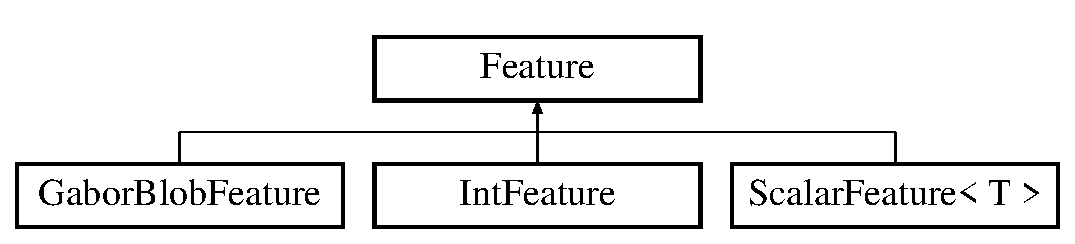
\includegraphics[height=2.000000cm]{class_feature}
\end{center}
\end{figure}
\subsection*{Public Member Functions}
\begin{DoxyCompactItemize}
\item 
\hyperlink{class_feature_a0a781cf57089800686f88e27c50cb313}{Feature} (void)
\item 
\hyperlink{class_feature_ab6dfcfe22cc71c7b45a61d991b4ff775}{$\sim$\+Feature} (void)
\item 
virtual double \hyperlink{class_feature_a7dbbdc860cdc97bcd31584ae10dab3b1}{distance} (\hyperlink{class_feature}{Feature} $\ast$a)=0
\end{DoxyCompactItemize}


\subsection{Constructor \& Destructor Documentation}
\hypertarget{class_feature_a0a781cf57089800686f88e27c50cb313}{\index{Feature@{Feature}!Feature@{Feature}}
\index{Feature@{Feature}!Feature@{Feature}}
\subsubsection[{Feature}]{\setlength{\rightskip}{0pt plus 5cm}Feature\+::\+Feature (
\begin{DoxyParamCaption}
\item[{void}]{}
\end{DoxyParamCaption}
)\hspace{0.3cm}{\ttfamily [inline]}}}\label{class_feature_a0a781cf57089800686f88e27c50cb313}
\hypertarget{class_feature_ab6dfcfe22cc71c7b45a61d991b4ff775}{\index{Feature@{Feature}!````~Feature@{$\sim$\+Feature}}
\index{````~Feature@{$\sim$\+Feature}!Feature@{Feature}}
\subsubsection[{$\sim$\+Feature}]{\setlength{\rightskip}{0pt plus 5cm}Feature\+::$\sim$\+Feature (
\begin{DoxyParamCaption}
\item[{void}]{}
\end{DoxyParamCaption}
)\hspace{0.3cm}{\ttfamily [inline]}}}\label{class_feature_ab6dfcfe22cc71c7b45a61d991b4ff775}


\subsection{Member Function Documentation}
\hypertarget{class_feature_a7dbbdc860cdc97bcd31584ae10dab3b1}{\index{Feature@{Feature}!distance@{distance}}
\index{distance@{distance}!Feature@{Feature}}
\subsubsection[{distance}]{\setlength{\rightskip}{0pt plus 5cm}virtual double Feature\+::distance (
\begin{DoxyParamCaption}
\item[{{\bf Feature} $\ast$}]{a}
\end{DoxyParamCaption}
)\hspace{0.3cm}{\ttfamily [pure virtual]}}}\label{class_feature_a7dbbdc860cdc97bcd31584ae10dab3b1}


Implemented in \hyperlink{class_gabor_blob_feature_ac9dd690e58da5a3a1c1f1964c2949a7c}{Gabor\+Blob\+Feature}, \hyperlink{class_scalar_feature_a5b95859a0d7409d7d9306a0c262e8e17}{Scalar\+Feature$<$ T $>$}, and \hyperlink{class_int_feature_a629ca66179636f0e1e673b017fdbd95e}{Int\+Feature}.



The documentation for this class was generated from the following file\+:\begin{DoxyCompactItemize}
\item 
Manuscript\+App/\hyperlink{_feature_8h}{Feature.\+h}\end{DoxyCompactItemize}

\hypertarget{class_feature_extractor}{\section{Feature\+Extractor Class Reference}
\label{class_feature_extractor}\index{Feature\+Extractor@{Feature\+Extractor}}
}


{\ttfamily \#include $<$Feature\+Extractor.\+h$>$}

Inheritance diagram for Feature\+Extractor\+:\begin{figure}[H]
\begin{center}
\leavevmode
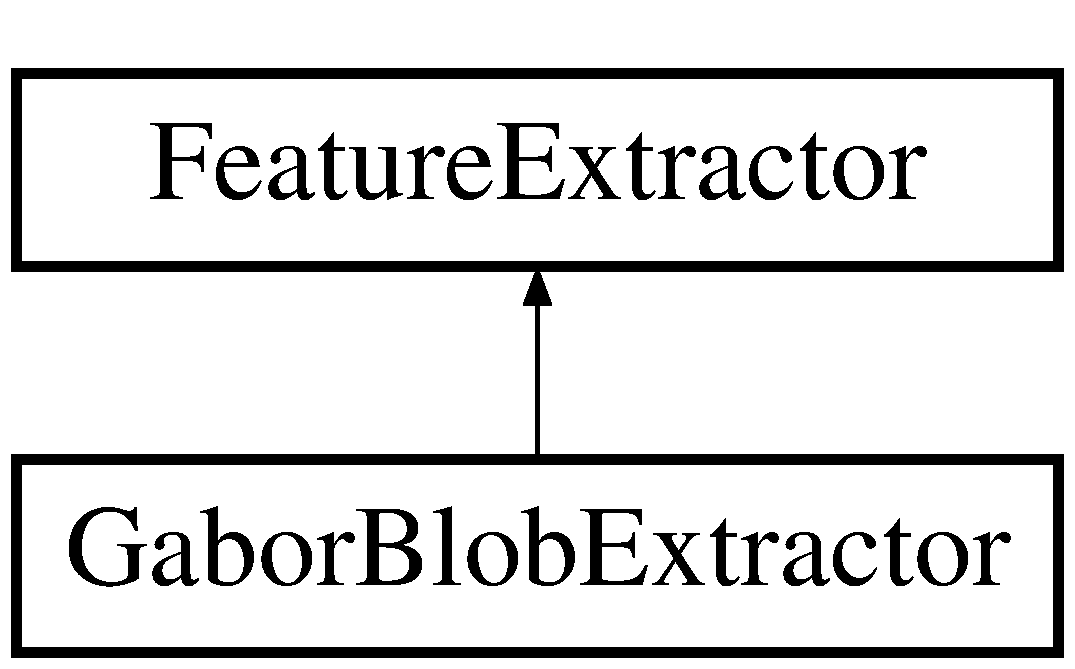
\includegraphics[height=2.000000cm]{class_feature_extractor}
\end{center}
\end{figure}
\subsection*{Public Member Functions}
\begin{DoxyCompactItemize}
\item 
\hyperlink{class_feature_extractor_a20fdc922c648855f2d6e4ba98377c2c0}{Feature\+Extractor} (void)
\item 
\hyperlink{class_feature_extractor_a69618427765f959e239836106f33dc61}{Feature\+Extractor} (Mat \&img)
\item 
\hyperlink{class_feature_extractor_ab659cba0f7ca31313ebf80544400dfae}{$\sim$\+Feature\+Extractor} (void)
\item 
void \hyperlink{class_feature_extractor_a2f56319a663c984edce8b3c977bf8b89}{set\+Image} (Mat \&img)
\item 
virtual void \hyperlink{class_feature_extractor_a34507279297dcc1bc8a7ba9422da4abf}{extract} (vector$<$ \hyperlink{class_feature}{Feature} $\ast$ $>$ \&)=0
\end{DoxyCompactItemize}
\subsection*{Protected Attributes}
\begin{DoxyCompactItemize}
\item 
Mat \hyperlink{class_feature_extractor_a56fefb5d4a1d14aef973442b4bf47a62}{\+\_\+image}
\end{DoxyCompactItemize}


\subsection{Constructor \& Destructor Documentation}
\hypertarget{class_feature_extractor_a20fdc922c648855f2d6e4ba98377c2c0}{\index{Feature\+Extractor@{Feature\+Extractor}!Feature\+Extractor@{Feature\+Extractor}}
\index{Feature\+Extractor@{Feature\+Extractor}!Feature\+Extractor@{Feature\+Extractor}}
\subsubsection[{Feature\+Extractor}]{\setlength{\rightskip}{0pt plus 5cm}Feature\+Extractor\+::\+Feature\+Extractor (
\begin{DoxyParamCaption}
\item[{void}]{}
\end{DoxyParamCaption}
)\hspace{0.3cm}{\ttfamily [inline]}}}\label{class_feature_extractor_a20fdc922c648855f2d6e4ba98377c2c0}
\hypertarget{class_feature_extractor_a69618427765f959e239836106f33dc61}{\index{Feature\+Extractor@{Feature\+Extractor}!Feature\+Extractor@{Feature\+Extractor}}
\index{Feature\+Extractor@{Feature\+Extractor}!Feature\+Extractor@{Feature\+Extractor}}
\subsubsection[{Feature\+Extractor}]{\setlength{\rightskip}{0pt plus 5cm}Feature\+Extractor\+::\+Feature\+Extractor (
\begin{DoxyParamCaption}
\item[{Mat \&}]{img}
\end{DoxyParamCaption}
)\hspace{0.3cm}{\ttfamily [inline]}}}\label{class_feature_extractor_a69618427765f959e239836106f33dc61}
\hypertarget{class_feature_extractor_ab659cba0f7ca31313ebf80544400dfae}{\index{Feature\+Extractor@{Feature\+Extractor}!````~Feature\+Extractor@{$\sim$\+Feature\+Extractor}}
\index{````~Feature\+Extractor@{$\sim$\+Feature\+Extractor}!Feature\+Extractor@{Feature\+Extractor}}
\subsubsection[{$\sim$\+Feature\+Extractor}]{\setlength{\rightskip}{0pt plus 5cm}Feature\+Extractor\+::$\sim$\+Feature\+Extractor (
\begin{DoxyParamCaption}
\item[{void}]{}
\end{DoxyParamCaption}
)\hspace{0.3cm}{\ttfamily [inline]}}}\label{class_feature_extractor_ab659cba0f7ca31313ebf80544400dfae}


\subsection{Member Function Documentation}
\hypertarget{class_feature_extractor_a34507279297dcc1bc8a7ba9422da4abf}{\index{Feature\+Extractor@{Feature\+Extractor}!extract@{extract}}
\index{extract@{extract}!Feature\+Extractor@{Feature\+Extractor}}
\subsubsection[{extract}]{\setlength{\rightskip}{0pt plus 5cm}virtual void Feature\+Extractor\+::extract (
\begin{DoxyParamCaption}
\item[{vector$<$ {\bf Feature} $\ast$ $>$ \&}]{}
\end{DoxyParamCaption}
)\hspace{0.3cm}{\ttfamily [pure virtual]}}}\label{class_feature_extractor_a34507279297dcc1bc8a7ba9422da4abf}


Implemented in \hyperlink{class_gabor_blob_extractor_aff19b47162d8d4244ac9325b82f1de4f}{Gabor\+Blob\+Extractor}.

\hypertarget{class_feature_extractor_a2f56319a663c984edce8b3c977bf8b89}{\index{Feature\+Extractor@{Feature\+Extractor}!set\+Image@{set\+Image}}
\index{set\+Image@{set\+Image}!Feature\+Extractor@{Feature\+Extractor}}
\subsubsection[{set\+Image}]{\setlength{\rightskip}{0pt plus 5cm}void Feature\+Extractor\+::set\+Image (
\begin{DoxyParamCaption}
\item[{Mat \&}]{img}
\end{DoxyParamCaption}
)\hspace{0.3cm}{\ttfamily [inline]}}}\label{class_feature_extractor_a2f56319a663c984edce8b3c977bf8b89}


\subsection{Member Data Documentation}
\hypertarget{class_feature_extractor_a56fefb5d4a1d14aef973442b4bf47a62}{\index{Feature\+Extractor@{Feature\+Extractor}!\+\_\+image@{\+\_\+image}}
\index{\+\_\+image@{\+\_\+image}!Feature\+Extractor@{Feature\+Extractor}}
\subsubsection[{\+\_\+image}]{\setlength{\rightskip}{0pt plus 5cm}Mat Feature\+Extractor\+::\+\_\+image\hspace{0.3cm}{\ttfamily [protected]}}}\label{class_feature_extractor_a56fefb5d4a1d14aef973442b4bf47a62}


The documentation for this class was generated from the following file\+:\begin{DoxyCompactItemize}
\item 
Manuscript\+App/\hyperlink{_feature_extractor_8h}{Feature\+Extractor.\+h}\end{DoxyCompactItemize}

\hypertarget{class_gabor_blob_extractor}{\section{Gabor\+Blob\+Extractor Class Reference}
\label{class_gabor_blob_extractor}\index{Gabor\+Blob\+Extractor@{Gabor\+Blob\+Extractor}}
}


{\ttfamily \#include $<$Gabor\+Blob\+Extractor.\+h$>$}

Inheritance diagram for Gabor\+Blob\+Extractor\+:\begin{figure}[H]
\begin{center}
\leavevmode
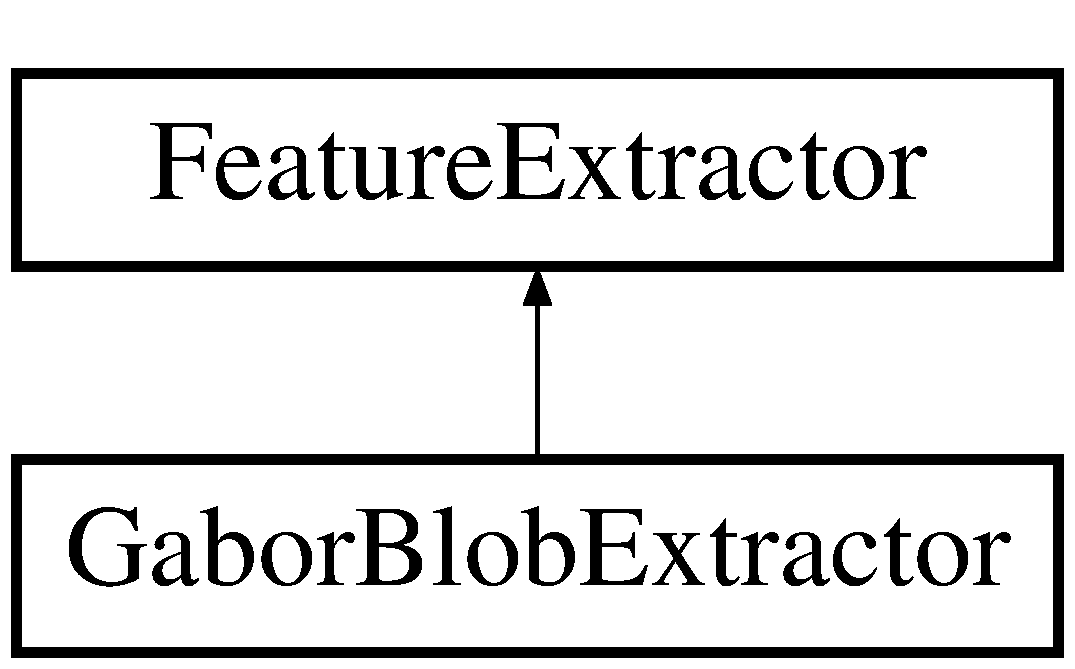
\includegraphics[height=2.000000cm]{class_gabor_blob_extractor}
\end{center}
\end{figure}
\subsection*{Public Member Functions}
\begin{DoxyCompactItemize}
\item 
\hyperlink{class_gabor_blob_extractor_a7f3a5a4c61cd515fbae56fdfefe3d004}{Gabor\+Blob\+Extractor} ()
\item 
\hyperlink{class_gabor_blob_extractor_a5c911de75dbda420e572cf1715440bb1}{Gabor\+Blob\+Extractor} (int n, int r, double sigma, double lambda)
\item 
\hyperlink{class_gabor_blob_extractor_ac13442f2a5ca9d980efb4ed93c6576f6}{$\sim$\+Gabor\+Blob\+Extractor} ()
\item 
void \hyperlink{class_gabor_blob_extractor_a033c00368027417ff74d14ce98e12108}{set\+Num\+Orientation} (int n)
\item 
\hyperlink{class_gabor_blob_feature}{Gabor\+Blob\+Feature} $\ast$ \hyperlink{class_gabor_blob_extractor_a9f332a64eaa87a97cd48fbc34a5a58da}{get\+Component\+Feature} (\hyperlink{class_connected_component}{Connected\+Component} $\ast$component)
\item 
void \hyperlink{class_gabor_blob_extractor_a8111b21c0587c91e53267bdcef9b1882}{process\+Response} (Mat \&response, vector$<$ \hyperlink{class_feature}{Feature} $\ast$ $>$ \&list)
\item 
void \hyperlink{class_gabor_blob_extractor_aff19b47162d8d4244ac9325b82f1de4f}{extract} (vector$<$ \hyperlink{class_feature}{Feature} $\ast$ $>$ \&)
\end{DoxyCompactItemize}
\subsection*{Additional Inherited Members}


\subsection{Constructor \& Destructor Documentation}
\hypertarget{class_gabor_blob_extractor_a7f3a5a4c61cd515fbae56fdfefe3d004}{\index{Gabor\+Blob\+Extractor@{Gabor\+Blob\+Extractor}!Gabor\+Blob\+Extractor@{Gabor\+Blob\+Extractor}}
\index{Gabor\+Blob\+Extractor@{Gabor\+Blob\+Extractor}!Gabor\+Blob\+Extractor@{Gabor\+Blob\+Extractor}}
\subsubsection[{Gabor\+Blob\+Extractor}]{\setlength{\rightskip}{0pt plus 5cm}Gabor\+Blob\+Extractor\+::\+Gabor\+Blob\+Extractor (
\begin{DoxyParamCaption}
{}
\end{DoxyParamCaption}
)\hspace{0.3cm}{\ttfamily [inline]}}}\label{class_gabor_blob_extractor_a7f3a5a4c61cd515fbae56fdfefe3d004}
\hypertarget{class_gabor_blob_extractor_a5c911de75dbda420e572cf1715440bb1}{\index{Gabor\+Blob\+Extractor@{Gabor\+Blob\+Extractor}!Gabor\+Blob\+Extractor@{Gabor\+Blob\+Extractor}}
\index{Gabor\+Blob\+Extractor@{Gabor\+Blob\+Extractor}!Gabor\+Blob\+Extractor@{Gabor\+Blob\+Extractor}}
\subsubsection[{Gabor\+Blob\+Extractor}]{\setlength{\rightskip}{0pt plus 5cm}Gabor\+Blob\+Extractor\+::\+Gabor\+Blob\+Extractor (
\begin{DoxyParamCaption}
\item[{int}]{n, }
\item[{int}]{r, }
\item[{double}]{sigma, }
\item[{double}]{lambda}
\end{DoxyParamCaption}
)\hspace{0.3cm}{\ttfamily [inline]}}}\label{class_gabor_blob_extractor_a5c911de75dbda420e572cf1715440bb1}
\hypertarget{class_gabor_blob_extractor_ac13442f2a5ca9d980efb4ed93c6576f6}{\index{Gabor\+Blob\+Extractor@{Gabor\+Blob\+Extractor}!````~Gabor\+Blob\+Extractor@{$\sim$\+Gabor\+Blob\+Extractor}}
\index{````~Gabor\+Blob\+Extractor@{$\sim$\+Gabor\+Blob\+Extractor}!Gabor\+Blob\+Extractor@{Gabor\+Blob\+Extractor}}
\subsubsection[{$\sim$\+Gabor\+Blob\+Extractor}]{\setlength{\rightskip}{0pt plus 5cm}Gabor\+Blob\+Extractor\+::$\sim$\+Gabor\+Blob\+Extractor (
\begin{DoxyParamCaption}
{}
\end{DoxyParamCaption}
)\hspace{0.3cm}{\ttfamily [inline]}}}\label{class_gabor_blob_extractor_ac13442f2a5ca9d980efb4ed93c6576f6}


\subsection{Member Function Documentation}
\hypertarget{class_gabor_blob_extractor_aff19b47162d8d4244ac9325b82f1de4f}{\index{Gabor\+Blob\+Extractor@{Gabor\+Blob\+Extractor}!extract@{extract}}
\index{extract@{extract}!Gabor\+Blob\+Extractor@{Gabor\+Blob\+Extractor}}
\subsubsection[{extract}]{\setlength{\rightskip}{0pt plus 5cm}void Gabor\+Blob\+Extractor\+::extract (
\begin{DoxyParamCaption}
\item[{vector$<$ {\bf Feature} $\ast$ $>$ \&}]{list}
\end{DoxyParamCaption}
)\hspace{0.3cm}{\ttfamily [virtual]}}}\label{class_gabor_blob_extractor_aff19b47162d8d4244ac9325b82f1de4f}


Implements \hyperlink{class_feature_extractor_a34507279297dcc1bc8a7ba9422da4abf}{Feature\+Extractor}.

\hypertarget{class_gabor_blob_extractor_a9f332a64eaa87a97cd48fbc34a5a58da}{\index{Gabor\+Blob\+Extractor@{Gabor\+Blob\+Extractor}!get\+Component\+Feature@{get\+Component\+Feature}}
\index{get\+Component\+Feature@{get\+Component\+Feature}!Gabor\+Blob\+Extractor@{Gabor\+Blob\+Extractor}}
\subsubsection[{get\+Component\+Feature}]{\setlength{\rightskip}{0pt plus 5cm}{\bf Gabor\+Blob\+Feature} $\ast$ Gabor\+Blob\+Extractor\+::get\+Component\+Feature (
\begin{DoxyParamCaption}
\item[{{\bf Connected\+Component} $\ast$}]{component}
\end{DoxyParamCaption}
)}}\label{class_gabor_blob_extractor_a9f332a64eaa87a97cd48fbc34a5a58da}
\hypertarget{class_gabor_blob_extractor_a8111b21c0587c91e53267bdcef9b1882}{\index{Gabor\+Blob\+Extractor@{Gabor\+Blob\+Extractor}!process\+Response@{process\+Response}}
\index{process\+Response@{process\+Response}!Gabor\+Blob\+Extractor@{Gabor\+Blob\+Extractor}}
\subsubsection[{process\+Response}]{\setlength{\rightskip}{0pt plus 5cm}void Gabor\+Blob\+Extractor\+::process\+Response (
\begin{DoxyParamCaption}
\item[{Mat \&}]{response, }
\item[{vector$<$ {\bf Feature} $\ast$ $>$ \&}]{list}
\end{DoxyParamCaption}
)}}\label{class_gabor_blob_extractor_a8111b21c0587c91e53267bdcef9b1882}
\hypertarget{class_gabor_blob_extractor_a033c00368027417ff74d14ce98e12108}{\index{Gabor\+Blob\+Extractor@{Gabor\+Blob\+Extractor}!set\+Num\+Orientation@{set\+Num\+Orientation}}
\index{set\+Num\+Orientation@{set\+Num\+Orientation}!Gabor\+Blob\+Extractor@{Gabor\+Blob\+Extractor}}
\subsubsection[{set\+Num\+Orientation}]{\setlength{\rightskip}{0pt plus 5cm}void Gabor\+Blob\+Extractor\+::set\+Num\+Orientation (
\begin{DoxyParamCaption}
\item[{int}]{n}
\end{DoxyParamCaption}
)\hspace{0.3cm}{\ttfamily [inline]}}}\label{class_gabor_blob_extractor_a033c00368027417ff74d14ce98e12108}


The documentation for this class was generated from the following files\+:\begin{DoxyCompactItemize}
\item 
Manuscript\+App/\hyperlink{_gabor_blob_extractor_8h}{Gabor\+Blob\+Extractor.\+h}\item 
Manuscript\+App/\hyperlink{_gabor_blob_extractor_8cpp}{Gabor\+Blob\+Extractor.\+cpp}\end{DoxyCompactItemize}

\hypertarget{class_gabor_blob_feature}{\section{Gabor\+Blob\+Feature Class Reference}
\label{class_gabor_blob_feature}\index{Gabor\+Blob\+Feature@{Gabor\+Blob\+Feature}}
}


{\ttfamily \#include $<$Gabor\+Blob\+Feature.\+h$>$}

Inheritance diagram for Gabor\+Blob\+Feature\+:\begin{figure}[H]
\begin{center}
\leavevmode
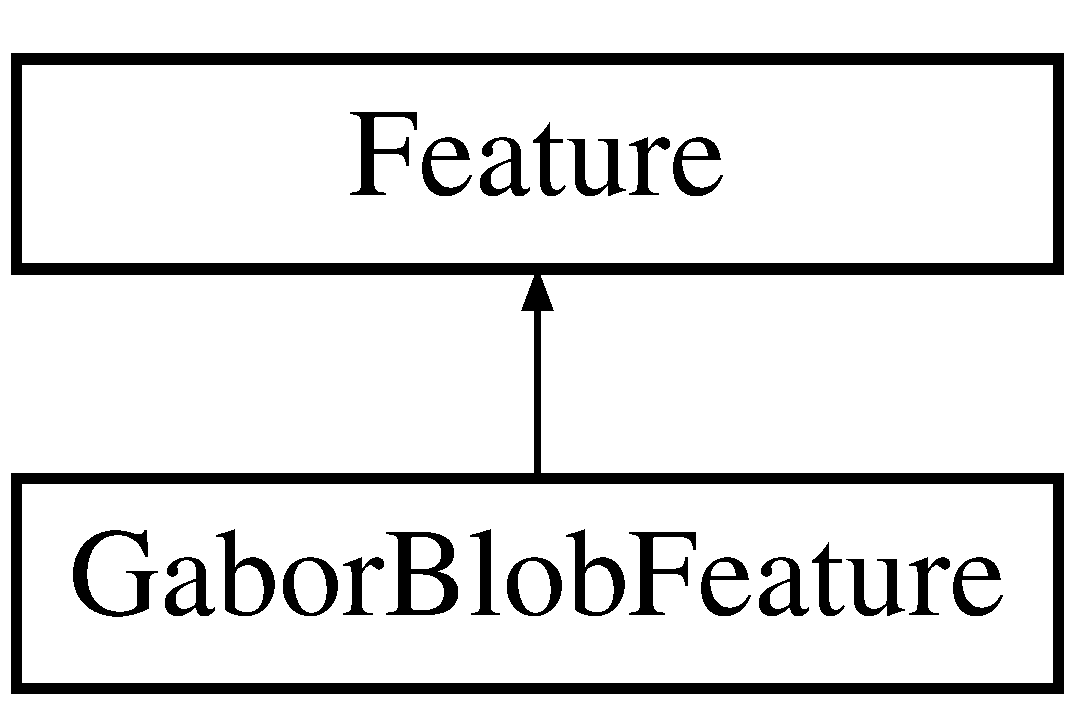
\includegraphics[height=2.000000cm]{class_gabor_blob_feature}
\end{center}
\end{figure}
\subsection*{Public Member Functions}
\begin{DoxyCompactItemize}
\item 
\hyperlink{class_gabor_blob_feature_a69e3ae10ed6cdd4d2a1263eccadf9c43}{Gabor\+Blob\+Feature} ()
\item 
\hyperlink{class_gabor_blob_feature_a3622476f0e482a1bae9efd0fe886f43b}{Gabor\+Blob\+Feature} (float \hyperlink{class_gabor_blob_feature_aeccf061ebe315eae8d9371cb0f80d3ed}{angle})
\item 
\hyperlink{class_gabor_blob_feature_a4e9516cce87a10ac9ae8094d6b00215f}{$\sim$\+Gabor\+Blob\+Feature} ()
\item 
void \hyperlink{class_gabor_blob_feature_aeccf061ebe315eae8d9371cb0f80d3ed}{angle} (float angle)
\item 
float \hyperlink{class_gabor_blob_feature_aab6f437b09cb5bb2788ea84dcb25ea9a}{angle} ()
\item 
void \hyperlink{class_gabor_blob_feature_ad3781ba28ee46dc9ee95481413d8f56a}{major\+Direction} (Point2f dir)
\item 
Point2f \hyperlink{class_gabor_blob_feature_a0e060ac23a33cc1edb3db7616c4ab818}{major\+Direction} ()
\item 
void \hyperlink{class_gabor_blob_feature_ac77bb0d685ec358947d98f2045950170}{minor\+Direction} (Point2f dir)
\item 
Point2f \hyperlink{class_gabor_blob_feature_ac68c416b9eb54df0e47421e86abd5bb6}{minor\+Direction} ()
\item 
void \hyperlink{class_gabor_blob_feature_a9494cf854702bf93ef07f169cbd65b01}{set\+Blob} (Mat \&mat)
\item 
Mat \& \hyperlink{class_gabor_blob_feature_aa501e837abb44fecf85e731147c97350}{get\+Blob} ()
\item 
void \hyperlink{class_gabor_blob_feature_a918d4aaee8cd2eda328d848f74431112}{set\+Samples} (Mat \&samples)
\item 
void \hyperlink{class_gabor_blob_feature_abe712f318a256f12d18a15ebf3fdf125}{compute\+Params} ()
\item 
double \hyperlink{class_gabor_blob_feature_ac9dd690e58da5a3a1c1f1964c2949a7c}{distance} (\hyperlink{class_feature}{Feature} $\ast$a)
\end{DoxyCompactItemize}


\subsection{Constructor \& Destructor Documentation}
\hypertarget{class_gabor_blob_feature_a69e3ae10ed6cdd4d2a1263eccadf9c43}{\index{Gabor\+Blob\+Feature@{Gabor\+Blob\+Feature}!Gabor\+Blob\+Feature@{Gabor\+Blob\+Feature}}
\index{Gabor\+Blob\+Feature@{Gabor\+Blob\+Feature}!Gabor\+Blob\+Feature@{Gabor\+Blob\+Feature}}
\subsubsection[{Gabor\+Blob\+Feature}]{\setlength{\rightskip}{0pt plus 5cm}Gabor\+Blob\+Feature\+::\+Gabor\+Blob\+Feature (
\begin{DoxyParamCaption}
{}
\end{DoxyParamCaption}
)\hspace{0.3cm}{\ttfamily [inline]}}}\label{class_gabor_blob_feature_a69e3ae10ed6cdd4d2a1263eccadf9c43}
\hypertarget{class_gabor_blob_feature_a3622476f0e482a1bae9efd0fe886f43b}{\index{Gabor\+Blob\+Feature@{Gabor\+Blob\+Feature}!Gabor\+Blob\+Feature@{Gabor\+Blob\+Feature}}
\index{Gabor\+Blob\+Feature@{Gabor\+Blob\+Feature}!Gabor\+Blob\+Feature@{Gabor\+Blob\+Feature}}
\subsubsection[{Gabor\+Blob\+Feature}]{\setlength{\rightskip}{0pt plus 5cm}Gabor\+Blob\+Feature\+::\+Gabor\+Blob\+Feature (
\begin{DoxyParamCaption}
\item[{float}]{angle}
\end{DoxyParamCaption}
)\hspace{0.3cm}{\ttfamily [inline]}}}\label{class_gabor_blob_feature_a3622476f0e482a1bae9efd0fe886f43b}
\hypertarget{class_gabor_blob_feature_a4e9516cce87a10ac9ae8094d6b00215f}{\index{Gabor\+Blob\+Feature@{Gabor\+Blob\+Feature}!````~Gabor\+Blob\+Feature@{$\sim$\+Gabor\+Blob\+Feature}}
\index{````~Gabor\+Blob\+Feature@{$\sim$\+Gabor\+Blob\+Feature}!Gabor\+Blob\+Feature@{Gabor\+Blob\+Feature}}
\subsubsection[{$\sim$\+Gabor\+Blob\+Feature}]{\setlength{\rightskip}{0pt plus 5cm}Gabor\+Blob\+Feature\+::$\sim$\+Gabor\+Blob\+Feature (
\begin{DoxyParamCaption}
{}
\end{DoxyParamCaption}
)\hspace{0.3cm}{\ttfamily [inline]}}}\label{class_gabor_blob_feature_a4e9516cce87a10ac9ae8094d6b00215f}


\subsection{Member Function Documentation}
\hypertarget{class_gabor_blob_feature_aeccf061ebe315eae8d9371cb0f80d3ed}{\index{Gabor\+Blob\+Feature@{Gabor\+Blob\+Feature}!angle@{angle}}
\index{angle@{angle}!Gabor\+Blob\+Feature@{Gabor\+Blob\+Feature}}
\subsubsection[{angle}]{\setlength{\rightskip}{0pt plus 5cm}void Gabor\+Blob\+Feature\+::angle (
\begin{DoxyParamCaption}
\item[{float}]{angle}
\end{DoxyParamCaption}
)\hspace{0.3cm}{\ttfamily [inline]}}}\label{class_gabor_blob_feature_aeccf061ebe315eae8d9371cb0f80d3ed}
\hypertarget{class_gabor_blob_feature_aab6f437b09cb5bb2788ea84dcb25ea9a}{\index{Gabor\+Blob\+Feature@{Gabor\+Blob\+Feature}!angle@{angle}}
\index{angle@{angle}!Gabor\+Blob\+Feature@{Gabor\+Blob\+Feature}}
\subsubsection[{angle}]{\setlength{\rightskip}{0pt plus 5cm}float Gabor\+Blob\+Feature\+::angle (
\begin{DoxyParamCaption}
{}
\end{DoxyParamCaption}
)\hspace{0.3cm}{\ttfamily [inline]}}}\label{class_gabor_blob_feature_aab6f437b09cb5bb2788ea84dcb25ea9a}
\hypertarget{class_gabor_blob_feature_abe712f318a256f12d18a15ebf3fdf125}{\index{Gabor\+Blob\+Feature@{Gabor\+Blob\+Feature}!compute\+Params@{compute\+Params}}
\index{compute\+Params@{compute\+Params}!Gabor\+Blob\+Feature@{Gabor\+Blob\+Feature}}
\subsubsection[{compute\+Params}]{\setlength{\rightskip}{0pt plus 5cm}void Gabor\+Blob\+Feature\+::compute\+Params (
\begin{DoxyParamCaption}
{}
\end{DoxyParamCaption}
)}}\label{class_gabor_blob_feature_abe712f318a256f12d18a15ebf3fdf125}
\hypertarget{class_gabor_blob_feature_ac9dd690e58da5a3a1c1f1964c2949a7c}{\index{Gabor\+Blob\+Feature@{Gabor\+Blob\+Feature}!distance@{distance}}
\index{distance@{distance}!Gabor\+Blob\+Feature@{Gabor\+Blob\+Feature}}
\subsubsection[{distance}]{\setlength{\rightskip}{0pt plus 5cm}double Gabor\+Blob\+Feature\+::distance (
\begin{DoxyParamCaption}
\item[{{\bf Feature} $\ast$}]{a}
\end{DoxyParamCaption}
)\hspace{0.3cm}{\ttfamily [virtual]}}}\label{class_gabor_blob_feature_ac9dd690e58da5a3a1c1f1964c2949a7c}


Implements \hyperlink{class_feature_a7dbbdc860cdc97bcd31584ae10dab3b1}{Feature}.

\hypertarget{class_gabor_blob_feature_aa501e837abb44fecf85e731147c97350}{\index{Gabor\+Blob\+Feature@{Gabor\+Blob\+Feature}!get\+Blob@{get\+Blob}}
\index{get\+Blob@{get\+Blob}!Gabor\+Blob\+Feature@{Gabor\+Blob\+Feature}}
\subsubsection[{get\+Blob}]{\setlength{\rightskip}{0pt plus 5cm}Mat\& Gabor\+Blob\+Feature\+::get\+Blob (
\begin{DoxyParamCaption}
{}
\end{DoxyParamCaption}
)\hspace{0.3cm}{\ttfamily [inline]}}}\label{class_gabor_blob_feature_aa501e837abb44fecf85e731147c97350}
\hypertarget{class_gabor_blob_feature_ad3781ba28ee46dc9ee95481413d8f56a}{\index{Gabor\+Blob\+Feature@{Gabor\+Blob\+Feature}!major\+Direction@{major\+Direction}}
\index{major\+Direction@{major\+Direction}!Gabor\+Blob\+Feature@{Gabor\+Blob\+Feature}}
\subsubsection[{major\+Direction}]{\setlength{\rightskip}{0pt plus 5cm}void Gabor\+Blob\+Feature\+::major\+Direction (
\begin{DoxyParamCaption}
\item[{Point2f}]{dir}
\end{DoxyParamCaption}
)\hspace{0.3cm}{\ttfamily [inline]}}}\label{class_gabor_blob_feature_ad3781ba28ee46dc9ee95481413d8f56a}
\hypertarget{class_gabor_blob_feature_a0e060ac23a33cc1edb3db7616c4ab818}{\index{Gabor\+Blob\+Feature@{Gabor\+Blob\+Feature}!major\+Direction@{major\+Direction}}
\index{major\+Direction@{major\+Direction}!Gabor\+Blob\+Feature@{Gabor\+Blob\+Feature}}
\subsubsection[{major\+Direction}]{\setlength{\rightskip}{0pt plus 5cm}Point2f Gabor\+Blob\+Feature\+::major\+Direction (
\begin{DoxyParamCaption}
{}
\end{DoxyParamCaption}
)\hspace{0.3cm}{\ttfamily [inline]}}}\label{class_gabor_blob_feature_a0e060ac23a33cc1edb3db7616c4ab818}
\hypertarget{class_gabor_blob_feature_ac77bb0d685ec358947d98f2045950170}{\index{Gabor\+Blob\+Feature@{Gabor\+Blob\+Feature}!minor\+Direction@{minor\+Direction}}
\index{minor\+Direction@{minor\+Direction}!Gabor\+Blob\+Feature@{Gabor\+Blob\+Feature}}
\subsubsection[{minor\+Direction}]{\setlength{\rightskip}{0pt plus 5cm}void Gabor\+Blob\+Feature\+::minor\+Direction (
\begin{DoxyParamCaption}
\item[{Point2f}]{dir}
\end{DoxyParamCaption}
)\hspace{0.3cm}{\ttfamily [inline]}}}\label{class_gabor_blob_feature_ac77bb0d685ec358947d98f2045950170}
\hypertarget{class_gabor_blob_feature_ac68c416b9eb54df0e47421e86abd5bb6}{\index{Gabor\+Blob\+Feature@{Gabor\+Blob\+Feature}!minor\+Direction@{minor\+Direction}}
\index{minor\+Direction@{minor\+Direction}!Gabor\+Blob\+Feature@{Gabor\+Blob\+Feature}}
\subsubsection[{minor\+Direction}]{\setlength{\rightskip}{0pt plus 5cm}Point2f Gabor\+Blob\+Feature\+::minor\+Direction (
\begin{DoxyParamCaption}
{}
\end{DoxyParamCaption}
)\hspace{0.3cm}{\ttfamily [inline]}}}\label{class_gabor_blob_feature_ac68c416b9eb54df0e47421e86abd5bb6}
\hypertarget{class_gabor_blob_feature_a9494cf854702bf93ef07f169cbd65b01}{\index{Gabor\+Blob\+Feature@{Gabor\+Blob\+Feature}!set\+Blob@{set\+Blob}}
\index{set\+Blob@{set\+Blob}!Gabor\+Blob\+Feature@{Gabor\+Blob\+Feature}}
\subsubsection[{set\+Blob}]{\setlength{\rightskip}{0pt plus 5cm}void Gabor\+Blob\+Feature\+::set\+Blob (
\begin{DoxyParamCaption}
\item[{Mat \&}]{mat}
\end{DoxyParamCaption}
)\hspace{0.3cm}{\ttfamily [inline]}}}\label{class_gabor_blob_feature_a9494cf854702bf93ef07f169cbd65b01}
\hypertarget{class_gabor_blob_feature_a918d4aaee8cd2eda328d848f74431112}{\index{Gabor\+Blob\+Feature@{Gabor\+Blob\+Feature}!set\+Samples@{set\+Samples}}
\index{set\+Samples@{set\+Samples}!Gabor\+Blob\+Feature@{Gabor\+Blob\+Feature}}
\subsubsection[{set\+Samples}]{\setlength{\rightskip}{0pt plus 5cm}void Gabor\+Blob\+Feature\+::set\+Samples (
\begin{DoxyParamCaption}
\item[{Mat \&}]{samples}
\end{DoxyParamCaption}
)}}\label{class_gabor_blob_feature_a918d4aaee8cd2eda328d848f74431112}


The documentation for this class was generated from the following files\+:\begin{DoxyCompactItemize}
\item 
Manuscript\+App/\hyperlink{_gabor_blob_feature_8h}{Gabor\+Blob\+Feature.\+h}\item 
Manuscript\+App/\hyperlink{_gabor_blob_feature_8cpp}{Gabor\+Blob\+Feature.\+cpp}\end{DoxyCompactItemize}

\hypertarget{class_global_binarizer}{\section{Global\+Binarizer Class Reference}
\label{class_global_binarizer}\index{Global\+Binarizer@{Global\+Binarizer}}
}


Global binarizer implment a global binarization algorithm  




{\ttfamily \#include $<$Global\+Binarizer.\+h$>$}

Inheritance diagram for Global\+Binarizer\+:\begin{figure}[H]
\begin{center}
\leavevmode
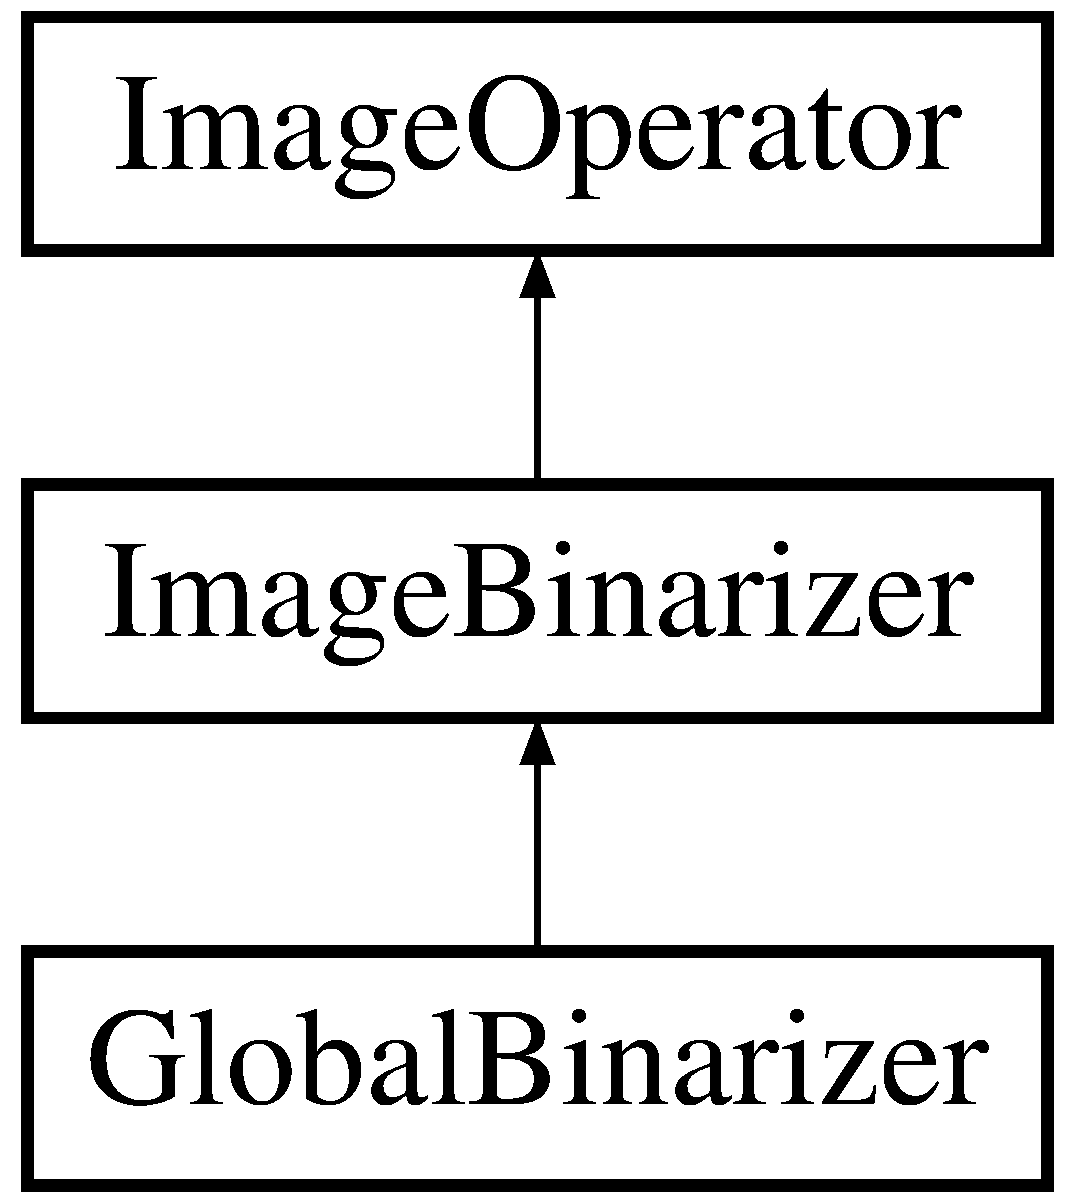
\includegraphics[height=3.000000cm]{class_global_binarizer}
\end{center}
\end{figure}
\subsection*{Public Member Functions}
\begin{DoxyCompactItemize}
\item 
\hyperlink{class_global_binarizer_a50bbd8c67da42e27dcecfcbacfa1189d}{Global\+Binarizer} (void)
\item 
\hyperlink{class_global_binarizer_a737f40337f87b8dc84f75aff325ee748}{Global\+Binarizer} (float thershold)
\item 
\hyperlink{class_global_binarizer_ad5f62437210fb6c174db58456b09c632}{$\sim$\+Global\+Binarizer} (void)
\item 
void \hyperlink{class_global_binarizer_a68d1645debe43e1142b922b7206e6b28}{set\+Thershold} (float threshold)
\item 
\hyperlink{class_d_image}{D\+Image} $\ast$ \hyperlink{class_global_binarizer_ad553b71737ff73e4ec06ccc52ba01b25}{binarize} ()
\begin{DoxyCompactList}\small\item\em Binarize the image using an input threshold \+\_\+thershold. \end{DoxyCompactList}\end{DoxyCompactItemize}
\subsection*{Additional Inherited Members}


\subsection{Detailed Description}
Global binarizer implment a global binarization algorithm 

El Sana, 2/15/2012. 

\subsection{Constructor \& Destructor Documentation}
\hypertarget{class_global_binarizer_a50bbd8c67da42e27dcecfcbacfa1189d}{\index{Global\+Binarizer@{Global\+Binarizer}!Global\+Binarizer@{Global\+Binarizer}}
\index{Global\+Binarizer@{Global\+Binarizer}!Global\+Binarizer@{Global\+Binarizer}}
\subsubsection[{Global\+Binarizer}]{\setlength{\rightskip}{0pt plus 5cm}Global\+Binarizer\+::\+Global\+Binarizer (
\begin{DoxyParamCaption}
\item[{void}]{}
\end{DoxyParamCaption}
)}}\label{class_global_binarizer_a50bbd8c67da42e27dcecfcbacfa1189d}
\hypertarget{class_global_binarizer_a737f40337f87b8dc84f75aff325ee748}{\index{Global\+Binarizer@{Global\+Binarizer}!Global\+Binarizer@{Global\+Binarizer}}
\index{Global\+Binarizer@{Global\+Binarizer}!Global\+Binarizer@{Global\+Binarizer}}
\subsubsection[{Global\+Binarizer}]{\setlength{\rightskip}{0pt plus 5cm}Global\+Binarizer\+::\+Global\+Binarizer (
\begin{DoxyParamCaption}
\item[{float}]{thershold}
\end{DoxyParamCaption}
)}}\label{class_global_binarizer_a737f40337f87b8dc84f75aff325ee748}
\hypertarget{class_global_binarizer_ad5f62437210fb6c174db58456b09c632}{\index{Global\+Binarizer@{Global\+Binarizer}!````~Global\+Binarizer@{$\sim$\+Global\+Binarizer}}
\index{````~Global\+Binarizer@{$\sim$\+Global\+Binarizer}!Global\+Binarizer@{Global\+Binarizer}}
\subsubsection[{$\sim$\+Global\+Binarizer}]{\setlength{\rightskip}{0pt plus 5cm}Global\+Binarizer\+::$\sim$\+Global\+Binarizer (
\begin{DoxyParamCaption}
\item[{void}]{}
\end{DoxyParamCaption}
)}}\label{class_global_binarizer_ad5f62437210fb6c174db58456b09c632}


\subsection{Member Function Documentation}
\hypertarget{class_global_binarizer_ad553b71737ff73e4ec06ccc52ba01b25}{\index{Global\+Binarizer@{Global\+Binarizer}!binarize@{binarize}}
\index{binarize@{binarize}!Global\+Binarizer@{Global\+Binarizer}}
\subsubsection[{binarize}]{\setlength{\rightskip}{0pt plus 5cm}{\bf D\+Image} $\ast$ Global\+Binarizer\+::binarize (
\begin{DoxyParamCaption}
{}
\end{DoxyParamCaption}
)\hspace{0.3cm}{\ttfamily [virtual]}}}\label{class_global_binarizer_ad553b71737ff73e4ec06ccc52ba01b25}


Binarize the image using an input threshold \+\_\+thershold. 

El Sana, 2/15/2012. 

\begin{DoxyReturn}{Returns}
null if it fails, else. 
\end{DoxyReturn}


Implements \hyperlink{class_image_binarizer_accf059357ade25887a94c91f76262254}{Image\+Binarizer}.

\hypertarget{class_global_binarizer_a68d1645debe43e1142b922b7206e6b28}{\index{Global\+Binarizer@{Global\+Binarizer}!set\+Thershold@{set\+Thershold}}
\index{set\+Thershold@{set\+Thershold}!Global\+Binarizer@{Global\+Binarizer}}
\subsubsection[{set\+Thershold}]{\setlength{\rightskip}{0pt plus 5cm}void Global\+Binarizer\+::set\+Thershold (
\begin{DoxyParamCaption}
\item[{float}]{threshold}
\end{DoxyParamCaption}
)\hspace{0.3cm}{\ttfamily [inline]}}}\label{class_global_binarizer_a68d1645debe43e1142b922b7206e6b28}


The documentation for this class was generated from the following files\+:\begin{DoxyCompactItemize}
\item 
Manuscript\+App/\hyperlink{_global_binarizer_8h}{Global\+Binarizer.\+h}\item 
Manuscript\+App/\hyperlink{_global_binarizer_8cpp}{Global\+Binarizer.\+cpp}\end{DoxyCompactItemize}

\hypertarget{class_histogram}{\section{Histogram Class Reference}
\label{class_histogram}\index{Histogram@{Histogram}}
}


{\ttfamily \#include $<$Histogram.\+h$>$}

\subsection*{Public Member Functions}
\begin{DoxyCompactItemize}
\item 
\hyperlink{class_histogram_af7f6bdea94a9e6a44ca389d2a0f2cae2}{Histogram} (void)
\item 
\hyperlink{class_histogram_a6be99bbd12f2dfe12c38739166f37db2}{$\sim$\+Histogram} (void)
\item 
void \hyperlink{class_histogram_a46645826dac5764fa12488acf77fbc5f}{set} (Mat mat)
\item 
Mat \hyperlink{class_histogram_a182b34a7f9a0a23725029f4be34cea0f}{get} ()
\end{DoxyCompactItemize}


\subsection{Constructor \& Destructor Documentation}
\hypertarget{class_histogram_af7f6bdea94a9e6a44ca389d2a0f2cae2}{\index{Histogram@{Histogram}!Histogram@{Histogram}}
\index{Histogram@{Histogram}!Histogram@{Histogram}}
\subsubsection[{Histogram}]{\setlength{\rightskip}{0pt plus 5cm}Histogram\+::\+Histogram (
\begin{DoxyParamCaption}
\item[{void}]{}
\end{DoxyParamCaption}
)}}\label{class_histogram_af7f6bdea94a9e6a44ca389d2a0f2cae2}
\hypertarget{class_histogram_a6be99bbd12f2dfe12c38739166f37db2}{\index{Histogram@{Histogram}!````~Histogram@{$\sim$\+Histogram}}
\index{````~Histogram@{$\sim$\+Histogram}!Histogram@{Histogram}}
\subsubsection[{$\sim$\+Histogram}]{\setlength{\rightskip}{0pt plus 5cm}Histogram\+::$\sim$\+Histogram (
\begin{DoxyParamCaption}
\item[{void}]{}
\end{DoxyParamCaption}
)}}\label{class_histogram_a6be99bbd12f2dfe12c38739166f37db2}


\subsection{Member Function Documentation}
\hypertarget{class_histogram_a182b34a7f9a0a23725029f4be34cea0f}{\index{Histogram@{Histogram}!get@{get}}
\index{get@{get}!Histogram@{Histogram}}
\subsubsection[{get}]{\setlength{\rightskip}{0pt plus 5cm}Mat Histogram\+::get (
\begin{DoxyParamCaption}
{}
\end{DoxyParamCaption}
)\hspace{0.3cm}{\ttfamily [inline]}}}\label{class_histogram_a182b34a7f9a0a23725029f4be34cea0f}
\hypertarget{class_histogram_a46645826dac5764fa12488acf77fbc5f}{\index{Histogram@{Histogram}!set@{set}}
\index{set@{set}!Histogram@{Histogram}}
\subsubsection[{set}]{\setlength{\rightskip}{0pt plus 5cm}void Histogram\+::set (
\begin{DoxyParamCaption}
\item[{Mat}]{mat}
\end{DoxyParamCaption}
)\hspace{0.3cm}{\ttfamily [inline]}}}\label{class_histogram_a46645826dac5764fa12488acf77fbc5f}


The documentation for this class was generated from the following files\+:\begin{DoxyCompactItemize}
\item 
Manuscript\+App/\hyperlink{_histogram_8h}{Histogram.\+h}\item 
Manuscript\+App/\hyperlink{_histogram_8cpp}{Histogram.\+cpp}\end{DoxyCompactItemize}

\hypertarget{class_image_binarizer}{\section{Image\+Binarizer Class Reference}
\label{class_image_binarizer}\index{Image\+Binarizer@{Image\+Binarizer}}
}


{\ttfamily \#include $<$Image\+Binarizer.\+h$>$}

Inheritance diagram for Image\+Binarizer\+:\begin{figure}[H]
\begin{center}
\leavevmode
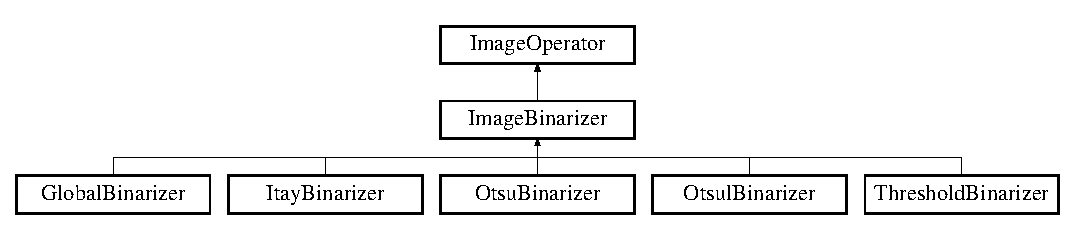
\includegraphics[height=2.645669cm]{class_image_binarizer}
\end{center}
\end{figure}
\subsection*{Public Member Functions}
\begin{DoxyCompactItemize}
\item 
virtual \hyperlink{class_d_image}{D\+Image} $\ast$ \hyperlink{class_image_binarizer_accf059357ade25887a94c91f76262254}{binarize} ()=0
\begin{DoxyCompactList}\small\item\em Binarize is the virtual function to implement a binarization algorithm in the extended class \end{DoxyCompactList}\end{DoxyCompactItemize}
\subsection*{Additional Inherited Members}


\subsection{Member Function Documentation}
\hypertarget{class_image_binarizer_accf059357ade25887a94c91f76262254}{\index{Image\+Binarizer@{Image\+Binarizer}!binarize@{binarize}}
\index{binarize@{binarize}!Image\+Binarizer@{Image\+Binarizer}}
\subsubsection[{binarize}]{\setlength{\rightskip}{0pt plus 5cm}virtual {\bf D\+Image}$\ast$ Image\+Binarizer\+::binarize (
\begin{DoxyParamCaption}
{}
\end{DoxyParamCaption}
)\hspace{0.3cm}{\ttfamily [pure virtual]}}}\label{class_image_binarizer_accf059357ade25887a94c91f76262254}


Binarize is the virtual function to implement a binarization algorithm in the extended class 

El Sana, 2/15/2012. 

\begin{DoxyReturn}{Returns}
null if it fails, else. 
\end{DoxyReturn}


Implemented in \hyperlink{class_threshold_binarizer_a2880414f620b4a6f44032e478217ee1e}{Threshold\+Binarizer}, \hyperlink{class_global_binarizer_ad553b71737ff73e4ec06ccc52ba01b25}{Global\+Binarizer}, \hyperlink{class_itay_binarizer_ad0093e357fe07cc4b42dcc2f0f416832}{Itay\+Binarizer}, \hyperlink{class_otsu_binarizer_a4219a9f9e72d1d0eceee30402bf2afd5}{Otsu\+Binarizer}, and \hyperlink{class_otsul_binarizer_a14064c86e424c1e68625b7fbc07195d5}{Otsul\+Binarizer}.



The documentation for this class was generated from the following file\+:\begin{DoxyCompactItemize}
\item 
Manuscript\+App/\hyperlink{_image_binarizer_8h}{Image\+Binarizer.\+h}\end{DoxyCompactItemize}

\hypertarget{class_image_converter}{\section{Image\+Converter Class Reference}
\label{class_image_converter}\index{Image\+Converter@{Image\+Converter}}
}


{\ttfamily \#include $<$Image\+Converter.\+h$>$}

Inheritance diagram for Image\+Converter\+:\begin{figure}[H]
\begin{center}
\leavevmode
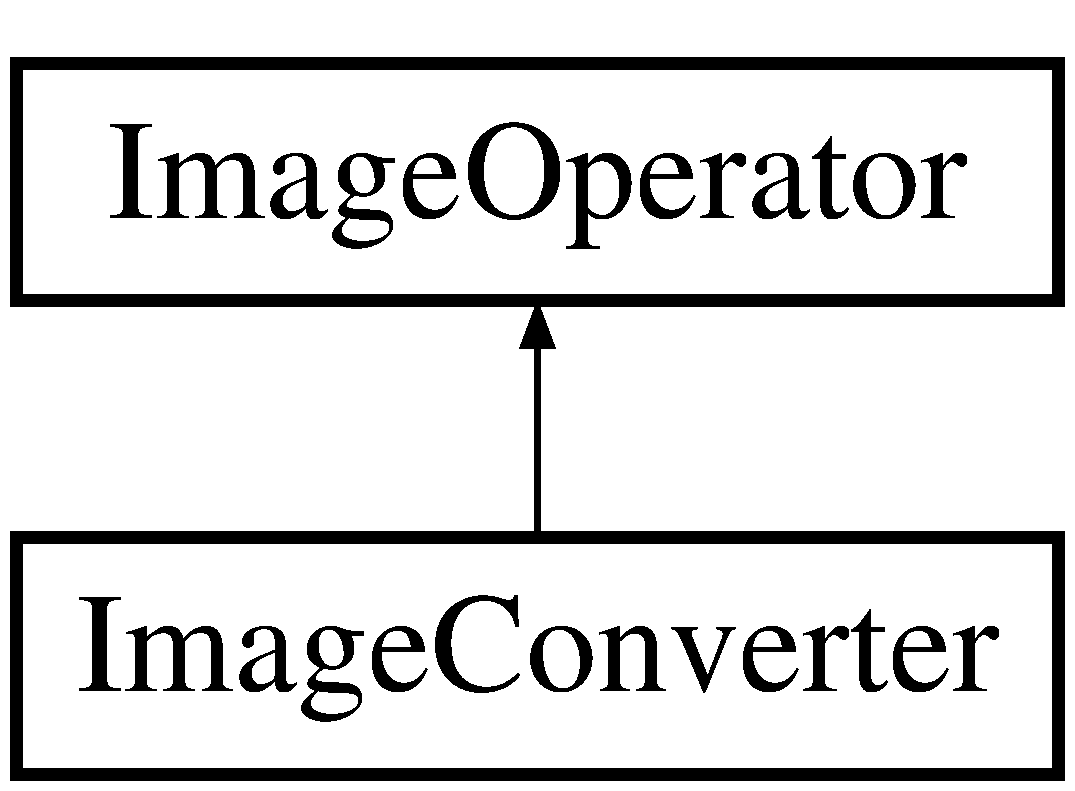
\includegraphics[height=2.000000cm]{class_image_converter}
\end{center}
\end{figure}
\subsection*{Public Member Functions}
\begin{DoxyCompactItemize}
\item 
\hyperlink{class_image_converter_abf8ca3f9d0c1f6eb86263086bbfdd54f}{Image\+Converter} (void)
\item 
\hyperlink{class_image_converter_a2f005d8140352d4a0befbef455e35e34}{$\sim$\+Image\+Converter} (void)
\item 
virtual \hyperlink{class_d_image}{D\+Image} $\ast$ \hyperlink{class_image_converter_ae318e984b77d5db5e3c37bbfd121b9dc}{convert} ()=0
\end{DoxyCompactItemize}
\subsection*{Additional Inherited Members}


\subsection{Constructor \& Destructor Documentation}
\hypertarget{class_image_converter_abf8ca3f9d0c1f6eb86263086bbfdd54f}{\index{Image\+Converter@{Image\+Converter}!Image\+Converter@{Image\+Converter}}
\index{Image\+Converter@{Image\+Converter}!Image\+Converter@{Image\+Converter}}
\subsubsection[{Image\+Converter}]{\setlength{\rightskip}{0pt plus 5cm}Image\+Converter\+::\+Image\+Converter (
\begin{DoxyParamCaption}
\item[{void}]{}
\end{DoxyParamCaption}
)}}\label{class_image_converter_abf8ca3f9d0c1f6eb86263086bbfdd54f}
\hypertarget{class_image_converter_a2f005d8140352d4a0befbef455e35e34}{\index{Image\+Converter@{Image\+Converter}!````~Image\+Converter@{$\sim$\+Image\+Converter}}
\index{````~Image\+Converter@{$\sim$\+Image\+Converter}!Image\+Converter@{Image\+Converter}}
\subsubsection[{$\sim$\+Image\+Converter}]{\setlength{\rightskip}{0pt plus 5cm}Image\+Converter\+::$\sim$\+Image\+Converter (
\begin{DoxyParamCaption}
\item[{void}]{}
\end{DoxyParamCaption}
)}}\label{class_image_converter_a2f005d8140352d4a0befbef455e35e34}


\subsection{Member Function Documentation}
\hypertarget{class_image_converter_ae318e984b77d5db5e3c37bbfd121b9dc}{\index{Image\+Converter@{Image\+Converter}!convert@{convert}}
\index{convert@{convert}!Image\+Converter@{Image\+Converter}}
\subsubsection[{convert}]{\setlength{\rightskip}{0pt plus 5cm}virtual {\bf D\+Image}$\ast$ Image\+Converter\+::convert (
\begin{DoxyParamCaption}
{}
\end{DoxyParamCaption}
)\hspace{0.3cm}{\ttfamily [pure virtual]}}}\label{class_image_converter_ae318e984b77d5db5e3c37bbfd121b9dc}


The documentation for this class was generated from the following files\+:\begin{DoxyCompactItemize}
\item 
Manuscript\+App/\hyperlink{_image_converter_8h}{Image\+Converter.\+h}\item 
Manuscript\+App/\hyperlink{_image_converter_8cpp}{Image\+Converter.\+cpp}\end{DoxyCompactItemize}

\hypertarget{class_image_enhancer}{\section{Image\+Enhancer Class Reference}
\label{class_image_enhancer}\index{Image\+Enhancer@{Image\+Enhancer}}
}


{\ttfamily \#include $<$Image\+Enhancer.\+h$>$}

Inheritance diagram for Image\+Enhancer\+:\begin{figure}[H]
\begin{center}
\leavevmode
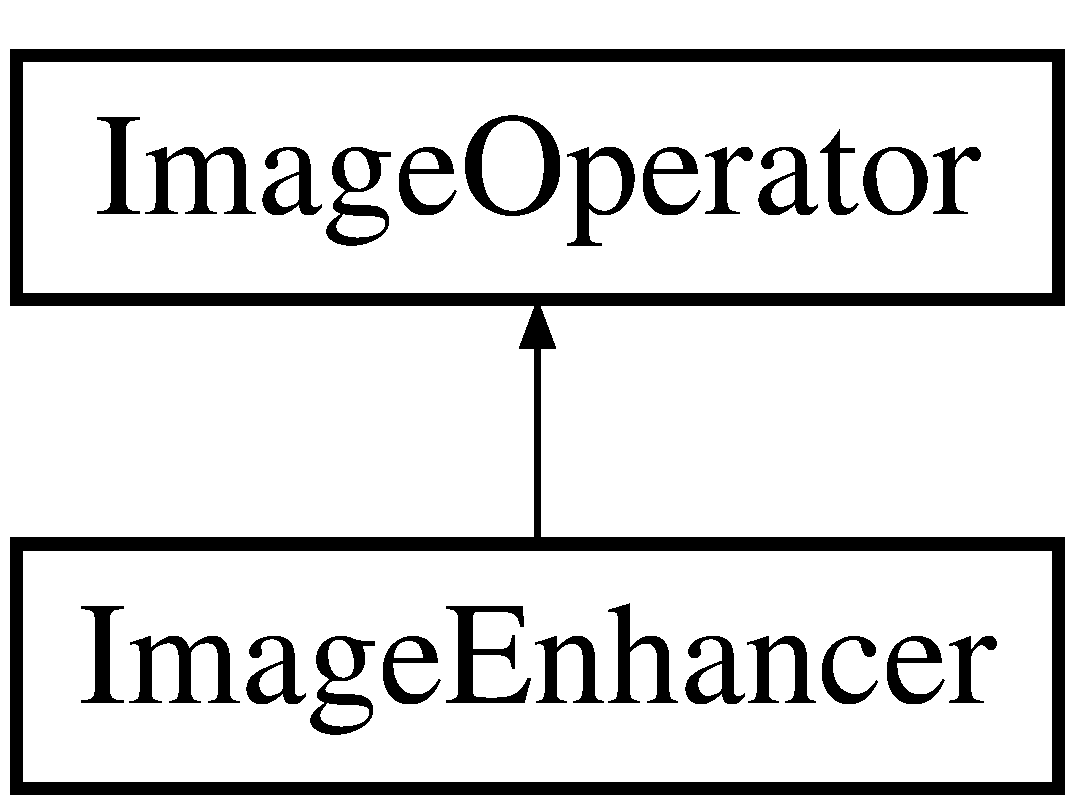
\includegraphics[height=2.000000cm]{class_image_enhancer}
\end{center}
\end{figure}
\subsection*{Public Member Functions}
\begin{DoxyCompactItemize}
\item 
virtual \hyperlink{class_d_image}{D\+Image} $\ast$ \hyperlink{class_image_enhancer_a1b46ef9f8e6271e0c7eb077ef2ac179f}{enhance} ()=0
\end{DoxyCompactItemize}
\subsection*{Additional Inherited Members}


\subsection{Member Function Documentation}
\hypertarget{class_image_enhancer_a1b46ef9f8e6271e0c7eb077ef2ac179f}{\index{Image\+Enhancer@{Image\+Enhancer}!enhance@{enhance}}
\index{enhance@{enhance}!Image\+Enhancer@{Image\+Enhancer}}
\subsubsection[{enhance}]{\setlength{\rightskip}{0pt plus 5cm}virtual {\bf D\+Image}$\ast$ Image\+Enhancer\+::enhance (
\begin{DoxyParamCaption}
{}
\end{DoxyParamCaption}
)\hspace{0.3cm}{\ttfamily [pure virtual]}}}\label{class_image_enhancer_a1b46ef9f8e6271e0c7eb077ef2ac179f}


The documentation for this class was generated from the following file\+:\begin{DoxyCompactItemize}
\item 
Manuscript\+App/\hyperlink{_image_enhancer_8h}{Image\+Enhancer.\+h}\end{DoxyCompactItemize}

\hypertarget{class_image_filter}{\section{Image\+Filter Class Reference}
\label{class_image_filter}\index{Image\+Filter@{Image\+Filter}}
}


{\ttfamily \#include $<$Image\+Filter.\+h$>$}

Inheritance diagram for Image\+Filter\+:\begin{figure}[H]
\begin{center}
\leavevmode
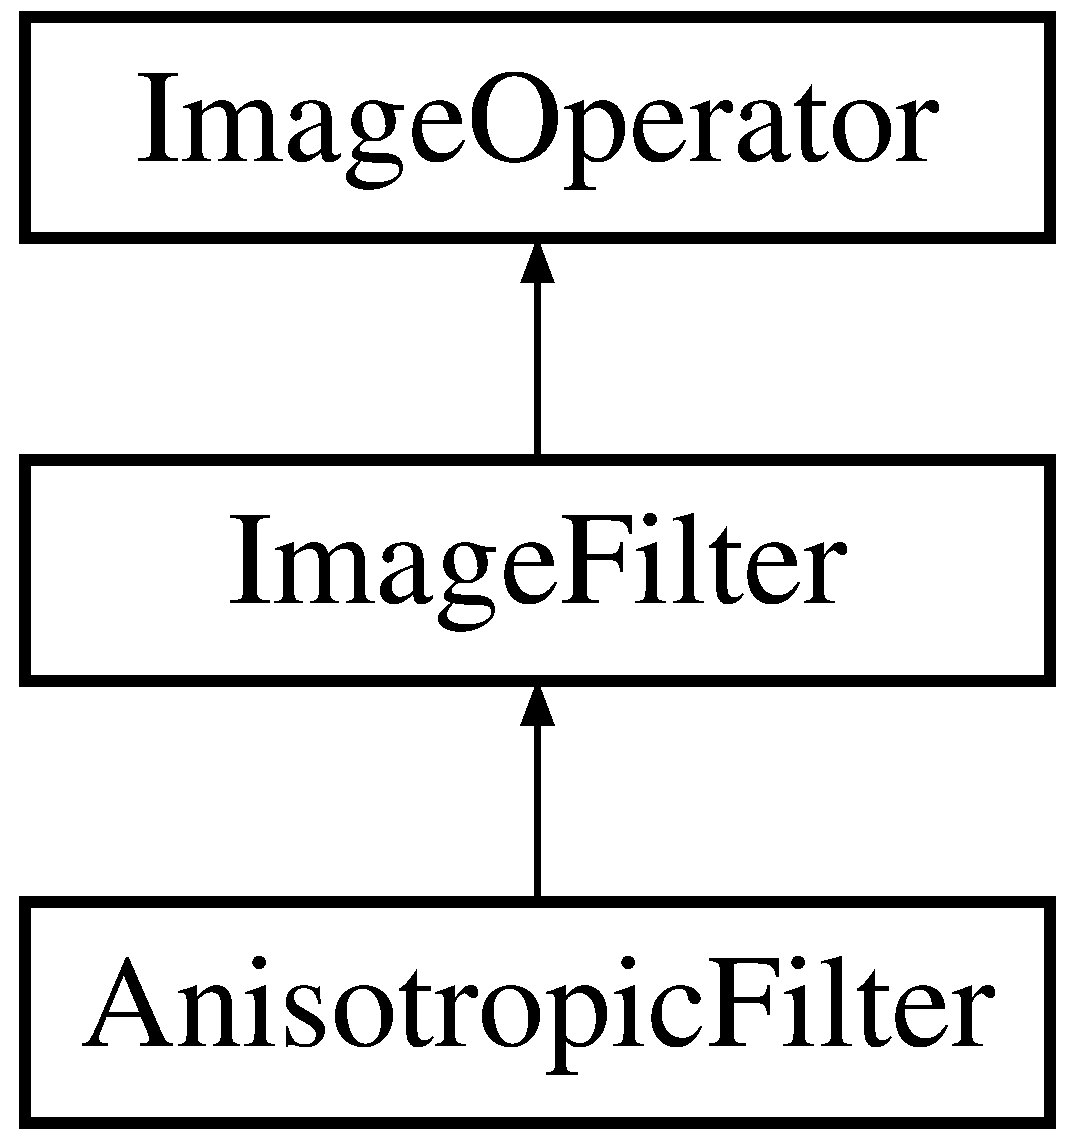
\includegraphics[height=3.000000cm]{class_image_filter}
\end{center}
\end{figure}
\subsection*{Public Member Functions}
\begin{DoxyCompactItemize}
\item 
\hyperlink{class_image_filter_a86dae480d07ddd441dc40c3ec89e5d3e}{Image\+Filter} (void)
\item 
\hyperlink{class_image_filter_a8d04f3e5a04c9b93cdbb004519161936}{$\sim$\+Image\+Filter} (void)
\item 
virtual \hyperlink{class_d_image}{D\+Image} $\ast$ \hyperlink{class_image_filter_afb06f41ef9470e2e2673eb3481c1f86a}{filter} ()=0
\end{DoxyCompactItemize}
\subsection*{Additional Inherited Members}


\subsection{Constructor \& Destructor Documentation}
\hypertarget{class_image_filter_a86dae480d07ddd441dc40c3ec89e5d3e}{\index{Image\+Filter@{Image\+Filter}!Image\+Filter@{Image\+Filter}}
\index{Image\+Filter@{Image\+Filter}!Image\+Filter@{Image\+Filter}}
\subsubsection[{Image\+Filter}]{\setlength{\rightskip}{0pt plus 5cm}Image\+Filter\+::\+Image\+Filter (
\begin{DoxyParamCaption}
\item[{void}]{}
\end{DoxyParamCaption}
)\hspace{0.3cm}{\ttfamily [inline]}}}\label{class_image_filter_a86dae480d07ddd441dc40c3ec89e5d3e}
\hypertarget{class_image_filter_a8d04f3e5a04c9b93cdbb004519161936}{\index{Image\+Filter@{Image\+Filter}!````~Image\+Filter@{$\sim$\+Image\+Filter}}
\index{````~Image\+Filter@{$\sim$\+Image\+Filter}!Image\+Filter@{Image\+Filter}}
\subsubsection[{$\sim$\+Image\+Filter}]{\setlength{\rightskip}{0pt plus 5cm}Image\+Filter\+::$\sim$\+Image\+Filter (
\begin{DoxyParamCaption}
\item[{void}]{}
\end{DoxyParamCaption}
)\hspace{0.3cm}{\ttfamily [inline]}}}\label{class_image_filter_a8d04f3e5a04c9b93cdbb004519161936}


\subsection{Member Function Documentation}
\hypertarget{class_image_filter_afb06f41ef9470e2e2673eb3481c1f86a}{\index{Image\+Filter@{Image\+Filter}!filter@{filter}}
\index{filter@{filter}!Image\+Filter@{Image\+Filter}}
\subsubsection[{filter}]{\setlength{\rightskip}{0pt plus 5cm}virtual {\bf D\+Image}$\ast$ Image\+Filter\+::filter (
\begin{DoxyParamCaption}
{}
\end{DoxyParamCaption}
)\hspace{0.3cm}{\ttfamily [pure virtual]}}}\label{class_image_filter_afb06f41ef9470e2e2673eb3481c1f86a}


Implemented in \hyperlink{class_anisotropic_filter_addbceed7b786a575f553bd4a41e0987c}{Anisotropic\+Filter}.



The documentation for this class was generated from the following file\+:\begin{DoxyCompactItemize}
\item 
Manuscript\+App/\hyperlink{_image_filter_8h}{Image\+Filter.\+h}\end{DoxyCompactItemize}

\hypertarget{class_image_operator}{\section{Image\+Operator Class Reference}
\label{class_image_operator}\index{Image\+Operator@{Image\+Operator}}
}


{\ttfamily \#include $<$Image\+Operator.\+h$>$}

Inheritance diagram for Image\+Operator\+:\begin{figure}[H]
\begin{center}
\leavevmode
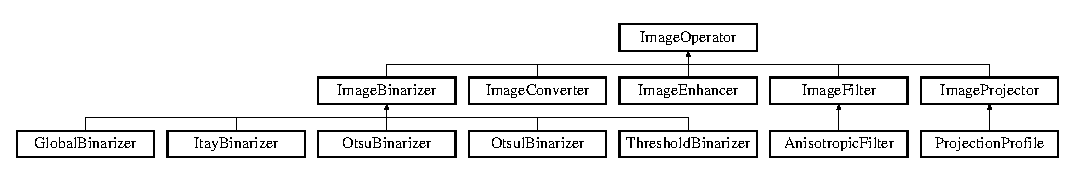
\includegraphics[height=1.889764cm]{class_image_operator}
\end{center}
\end{figure}
\subsection*{Public Member Functions}
\begin{DoxyCompactItemize}
\item 
\hyperlink{class_image_operator_ad51aedea73c2392a53dac0f359d67734}{Image\+Operator} (void)
\item 
\hyperlink{class_image_operator_aa21a419edd1071392438c98fec2bbb6b}{Image\+Operator} (\hyperlink{class_d_image}{D\+Image} $\ast$img)
\item 
\hyperlink{class_image_operator_a381d5ddd708a43730d9b0545b5fedff5}{$\sim$\+Image\+Operator} (void)
\item 
void \hyperlink{class_image_operator_a5b4f0975dabbfb1098d975dd238aa5d6}{set\+Image} (\hyperlink{class_d_image}{D\+Image} $\ast$img)
\begin{DoxyCompactList}\small\item\em Sets the operated image. \end{DoxyCompactList}\item 
\hyperlink{class_d_image}{D\+Image} $\ast$ \hyperlink{class_image_operator_a71271114184aa4d9fe21c903687b55a5}{get\+Image} ()
\begin{DoxyCompactList}\small\item\em Gets the operated image \end{DoxyCompactList}\end{DoxyCompactItemize}
\subsection*{Protected Attributes}
\begin{DoxyCompactItemize}
\item 
\hyperlink{class_d_image}{D\+Image} $\ast$ \hyperlink{class_image_operator_a096f8347c28e3c3e932d4bfe0fb33472}{\+\_\+image}
\end{DoxyCompactItemize}


\subsection{Constructor \& Destructor Documentation}
\hypertarget{class_image_operator_ad51aedea73c2392a53dac0f359d67734}{\index{Image\+Operator@{Image\+Operator}!Image\+Operator@{Image\+Operator}}
\index{Image\+Operator@{Image\+Operator}!Image\+Operator@{Image\+Operator}}
\subsubsection[{Image\+Operator}]{\setlength{\rightskip}{0pt plus 5cm}Image\+Operator\+::\+Image\+Operator (
\begin{DoxyParamCaption}
\item[{void}]{}
\end{DoxyParamCaption}
)\hspace{0.3cm}{\ttfamily [inline]}}}\label{class_image_operator_ad51aedea73c2392a53dac0f359d67734}
\hypertarget{class_image_operator_aa21a419edd1071392438c98fec2bbb6b}{\index{Image\+Operator@{Image\+Operator}!Image\+Operator@{Image\+Operator}}
\index{Image\+Operator@{Image\+Operator}!Image\+Operator@{Image\+Operator}}
\subsubsection[{Image\+Operator}]{\setlength{\rightskip}{0pt plus 5cm}Image\+Operator\+::\+Image\+Operator (
\begin{DoxyParamCaption}
\item[{{\bf D\+Image} $\ast$}]{img}
\end{DoxyParamCaption}
)\hspace{0.3cm}{\ttfamily [inline]}}}\label{class_image_operator_aa21a419edd1071392438c98fec2bbb6b}
\hypertarget{class_image_operator_a381d5ddd708a43730d9b0545b5fedff5}{\index{Image\+Operator@{Image\+Operator}!````~Image\+Operator@{$\sim$\+Image\+Operator}}
\index{````~Image\+Operator@{$\sim$\+Image\+Operator}!Image\+Operator@{Image\+Operator}}
\subsubsection[{$\sim$\+Image\+Operator}]{\setlength{\rightskip}{0pt plus 5cm}Image\+Operator\+::$\sim$\+Image\+Operator (
\begin{DoxyParamCaption}
\item[{void}]{}
\end{DoxyParamCaption}
)\hspace{0.3cm}{\ttfamily [inline]}}}\label{class_image_operator_a381d5ddd708a43730d9b0545b5fedff5}


\subsection{Member Function Documentation}
\hypertarget{class_image_operator_a71271114184aa4d9fe21c903687b55a5}{\index{Image\+Operator@{Image\+Operator}!get\+Image@{get\+Image}}
\index{get\+Image@{get\+Image}!Image\+Operator@{Image\+Operator}}
\subsubsection[{get\+Image}]{\setlength{\rightskip}{0pt plus 5cm}{\bf D\+Image}$\ast$ Image\+Operator\+::get\+Image (
\begin{DoxyParamCaption}
{}
\end{DoxyParamCaption}
)\hspace{0.3cm}{\ttfamily [inline]}}}\label{class_image_operator_a71271114184aa4d9fe21c903687b55a5}


Gets the operated image 

El Sana. 

\begin{DoxyReturn}{Returns}
The image. 
\end{DoxyReturn}
\hypertarget{class_image_operator_a5b4f0975dabbfb1098d975dd238aa5d6}{\index{Image\+Operator@{Image\+Operator}!set\+Image@{set\+Image}}
\index{set\+Image@{set\+Image}!Image\+Operator@{Image\+Operator}}
\subsubsection[{set\+Image}]{\setlength{\rightskip}{0pt plus 5cm}void Image\+Operator\+::set\+Image (
\begin{DoxyParamCaption}
\item[{{\bf D\+Image} $\ast$}]{img}
\end{DoxyParamCaption}
)\hspace{0.3cm}{\ttfamily [inline]}}}\label{class_image_operator_a5b4f0975dabbfb1098d975dd238aa5d6}


Sets the operated image. 

El Sana. 


\begin{DoxyParams}{Parameters}
{\em img} & \mbox{[}in\mbox{]} The image. \\
\hline
\end{DoxyParams}


\subsection{Member Data Documentation}
\hypertarget{class_image_operator_a096f8347c28e3c3e932d4bfe0fb33472}{\index{Image\+Operator@{Image\+Operator}!\+\_\+image@{\+\_\+image}}
\index{\+\_\+image@{\+\_\+image}!Image\+Operator@{Image\+Operator}}
\subsubsection[{\+\_\+image}]{\setlength{\rightskip}{0pt plus 5cm}{\bf D\+Image}$\ast$ Image\+Operator\+::\+\_\+image\hspace{0.3cm}{\ttfamily [protected]}}}\label{class_image_operator_a096f8347c28e3c3e932d4bfe0fb33472}


The documentation for this class was generated from the following file\+:\begin{DoxyCompactItemize}
\item 
Manuscript\+App/\hyperlink{_image_operator_8h}{Image\+Operator.\+h}\end{DoxyCompactItemize}

\hypertarget{class_image_projector}{\section{Image\+Projector Class Reference}
\label{class_image_projector}\index{Image\+Projector@{Image\+Projector}}
}


{\ttfamily \#include $<$Image\+Projector.\+h$>$}

Inheritance diagram for Image\+Projector\+:\begin{figure}[H]
\begin{center}
\leavevmode
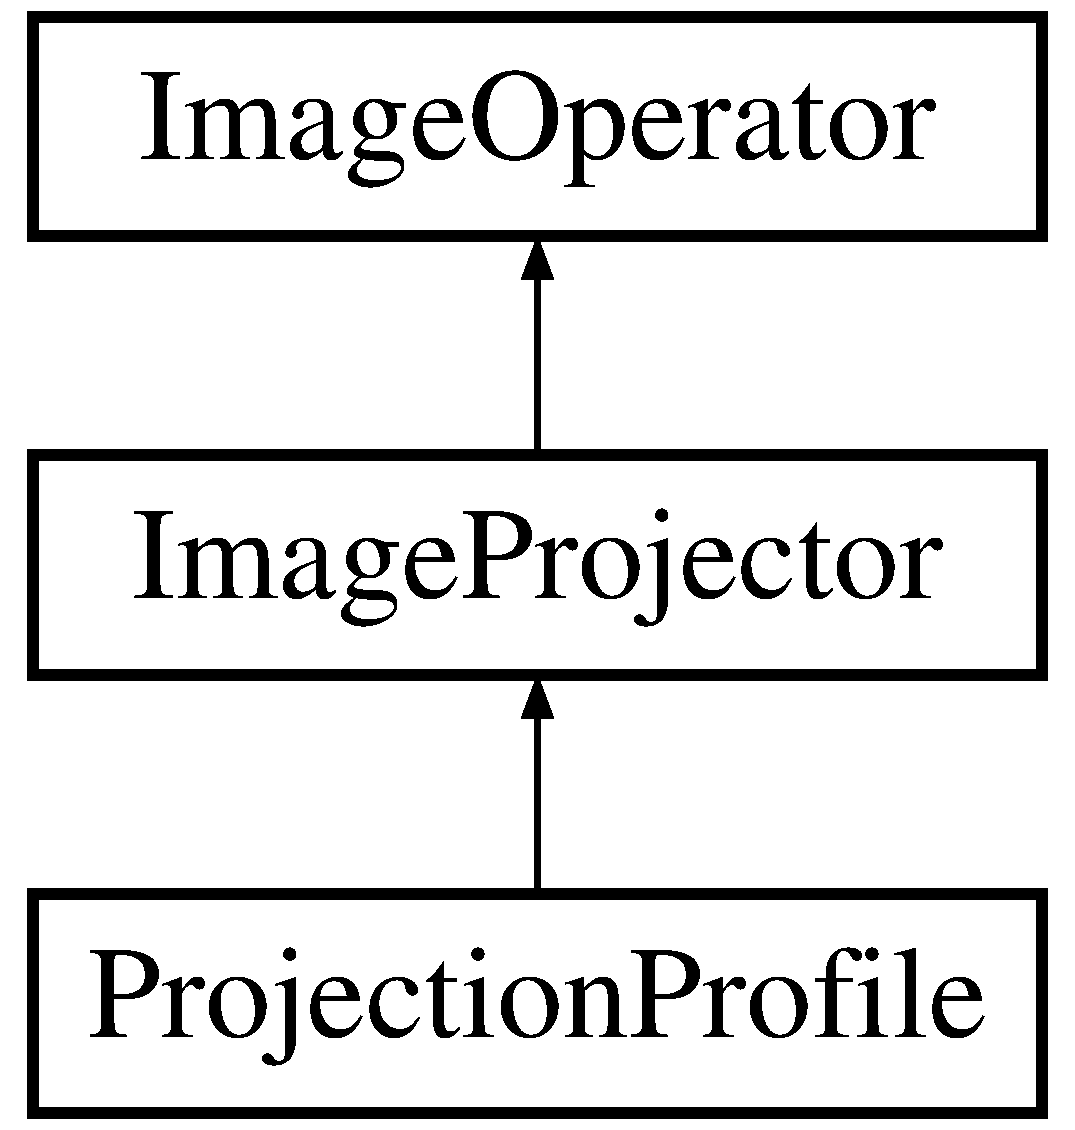
\includegraphics[height=3.000000cm]{class_image_projector}
\end{center}
\end{figure}
\subsection*{Public Member Functions}
\begin{DoxyCompactItemize}
\item 
virtual \hyperlink{class_d_image}{D\+Image} $\ast$ \hyperlink{class_image_projector_a3dd19fda98e15001d7cbf5b8ca1b4b40}{project} ()=0
\begin{DoxyCompactList}\small\item\em Project a 2\+D image into 1\+D image (one column) \end{DoxyCompactList}\end{DoxyCompactItemize}
\subsection*{Static Public Attributes}
\begin{DoxyCompactItemize}
\item 
static const int \hyperlink{class_image_projector_aa4f984418252e6203b04e4dcb5ab8183}{M\+O\+D\+E\+\_\+\+S\+U\+M} = 0
\item 
static const int \hyperlink{class_image_projector_a1f021faf00677be6e1bafdbf1f308ae2}{M\+O\+D\+E\+\_\+\+A\+V\+G} = 1
\item 
static const int \hyperlink{class_image_projector_a7b0d00775b3caaa86260c7e16771ef8d}{M\+O\+D\+E\+\_\+\+M\+A\+X} = 2
\item 
static const int \hyperlink{class_image_projector_a18c6aaf382882c18e38fba9058348d4b}{M\+O\+D\+E\+\_\+\+M\+I\+N} = 3
\end{DoxyCompactItemize}
\subsection*{Protected Attributes}
\begin{DoxyCompactItemize}
\item 
int \hyperlink{class_image_projector_ad23f3f3d0f5b2a66f07d543ec09a321e}{\+\_\+mode}
\item 
int \hyperlink{class_image_projector_a64c6fd5a87cef8bd941a84f45781fd1c}{\+\_\+direction}
\end{DoxyCompactItemize}


\subsection{Member Function Documentation}
\hypertarget{class_image_projector_a3dd19fda98e15001d7cbf5b8ca1b4b40}{\index{Image\+Projector@{Image\+Projector}!project@{project}}
\index{project@{project}!Image\+Projector@{Image\+Projector}}
\subsubsection[{project}]{\setlength{\rightskip}{0pt plus 5cm}virtual {\bf D\+Image}$\ast$ Image\+Projector\+::project (
\begin{DoxyParamCaption}
{}
\end{DoxyParamCaption}
)\hspace{0.3cm}{\ttfamily [pure virtual]}}}\label{class_image_projector_a3dd19fda98e15001d7cbf5b8ca1b4b40}


Project a 2\+D image into 1\+D image (one column) 

El Sana. 


\begin{DoxyParams}{Parameters}
{\em img} & \mbox{[}in\mbox{]} The image. \\
\hline
\end{DoxyParams}


Implemented in \hyperlink{class_projection_profile_a876b05a649f497584fe5d5632ffab9c0}{Projection\+Profile}.



\subsection{Member Data Documentation}
\hypertarget{class_image_projector_a64c6fd5a87cef8bd941a84f45781fd1c}{\index{Image\+Projector@{Image\+Projector}!\+\_\+direction@{\+\_\+direction}}
\index{\+\_\+direction@{\+\_\+direction}!Image\+Projector@{Image\+Projector}}
\subsubsection[{\+\_\+direction}]{\setlength{\rightskip}{0pt plus 5cm}int Image\+Projector\+::\+\_\+direction\hspace{0.3cm}{\ttfamily [protected]}}}\label{class_image_projector_a64c6fd5a87cef8bd941a84f45781fd1c}
\hypertarget{class_image_projector_ad23f3f3d0f5b2a66f07d543ec09a321e}{\index{Image\+Projector@{Image\+Projector}!\+\_\+mode@{\+\_\+mode}}
\index{\+\_\+mode@{\+\_\+mode}!Image\+Projector@{Image\+Projector}}
\subsubsection[{\+\_\+mode}]{\setlength{\rightskip}{0pt plus 5cm}int Image\+Projector\+::\+\_\+mode\hspace{0.3cm}{\ttfamily [protected]}}}\label{class_image_projector_ad23f3f3d0f5b2a66f07d543ec09a321e}
\hypertarget{class_image_projector_a1f021faf00677be6e1bafdbf1f308ae2}{\index{Image\+Projector@{Image\+Projector}!M\+O\+D\+E\+\_\+\+A\+V\+G@{M\+O\+D\+E\+\_\+\+A\+V\+G}}
\index{M\+O\+D\+E\+\_\+\+A\+V\+G@{M\+O\+D\+E\+\_\+\+A\+V\+G}!Image\+Projector@{Image\+Projector}}
\subsubsection[{M\+O\+D\+E\+\_\+\+A\+V\+G}]{\setlength{\rightskip}{0pt plus 5cm}const int Image\+Projector\+::\+M\+O\+D\+E\+\_\+\+A\+V\+G = 1\hspace{0.3cm}{\ttfamily [static]}}}\label{class_image_projector_a1f021faf00677be6e1bafdbf1f308ae2}
\hypertarget{class_image_projector_a7b0d00775b3caaa86260c7e16771ef8d}{\index{Image\+Projector@{Image\+Projector}!M\+O\+D\+E\+\_\+\+M\+A\+X@{M\+O\+D\+E\+\_\+\+M\+A\+X}}
\index{M\+O\+D\+E\+\_\+\+M\+A\+X@{M\+O\+D\+E\+\_\+\+M\+A\+X}!Image\+Projector@{Image\+Projector}}
\subsubsection[{M\+O\+D\+E\+\_\+\+M\+A\+X}]{\setlength{\rightskip}{0pt plus 5cm}const int Image\+Projector\+::\+M\+O\+D\+E\+\_\+\+M\+A\+X = 2\hspace{0.3cm}{\ttfamily [static]}}}\label{class_image_projector_a7b0d00775b3caaa86260c7e16771ef8d}
\hypertarget{class_image_projector_a18c6aaf382882c18e38fba9058348d4b}{\index{Image\+Projector@{Image\+Projector}!M\+O\+D\+E\+\_\+\+M\+I\+N@{M\+O\+D\+E\+\_\+\+M\+I\+N}}
\index{M\+O\+D\+E\+\_\+\+M\+I\+N@{M\+O\+D\+E\+\_\+\+M\+I\+N}!Image\+Projector@{Image\+Projector}}
\subsubsection[{M\+O\+D\+E\+\_\+\+M\+I\+N}]{\setlength{\rightskip}{0pt plus 5cm}const int Image\+Projector\+::\+M\+O\+D\+E\+\_\+\+M\+I\+N = 3\hspace{0.3cm}{\ttfamily [static]}}}\label{class_image_projector_a18c6aaf382882c18e38fba9058348d4b}
\hypertarget{class_image_projector_aa4f984418252e6203b04e4dcb5ab8183}{\index{Image\+Projector@{Image\+Projector}!M\+O\+D\+E\+\_\+\+S\+U\+M@{M\+O\+D\+E\+\_\+\+S\+U\+M}}
\index{M\+O\+D\+E\+\_\+\+S\+U\+M@{M\+O\+D\+E\+\_\+\+S\+U\+M}!Image\+Projector@{Image\+Projector}}
\subsubsection[{M\+O\+D\+E\+\_\+\+S\+U\+M}]{\setlength{\rightskip}{0pt plus 5cm}const int Image\+Projector\+::\+M\+O\+D\+E\+\_\+\+S\+U\+M = 0\hspace{0.3cm}{\ttfamily [static]}}}\label{class_image_projector_aa4f984418252e6203b04e4dcb5ab8183}


The documentation for this class was generated from the following file\+:\begin{DoxyCompactItemize}
\item 
Manuscript\+App/\hyperlink{_image_projector_8h}{Image\+Projector.\+h}\end{DoxyCompactItemize}

\hypertarget{class_int_feature}{\section{Int\+Feature Class Reference}
\label{class_int_feature}\index{Int\+Feature@{Int\+Feature}}
}


{\ttfamily \#include $<$Int\+Feature.\+h$>$}

Inheritance diagram for Int\+Feature\+:\begin{figure}[H]
\begin{center}
\leavevmode
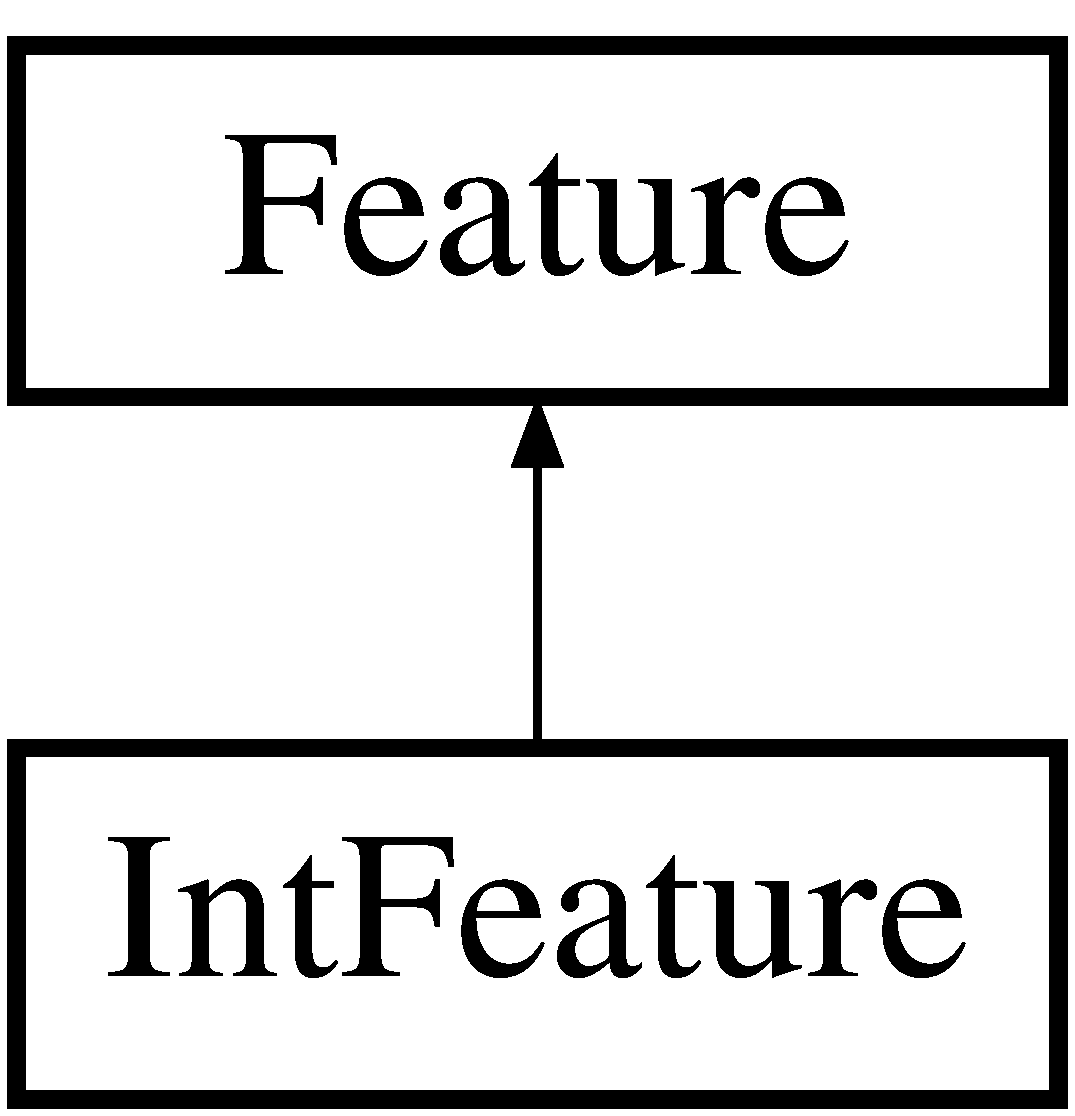
\includegraphics[height=2.000000cm]{class_int_feature}
\end{center}
\end{figure}
\subsection*{Public Member Functions}
\begin{DoxyCompactItemize}
\item 
\hyperlink{class_int_feature_accb2be99097e153df7abfde70894a9d2}{Int\+Feature} ()
\item 
\hyperlink{class_int_feature_aef75cf64b6b58c3b40b9ec607b8444f3}{Int\+Feature} (int a)
\item 
void \hyperlink{class_int_feature_aab965223e7190c970442ab059f8702ee}{val} (int a)
\item 
int \hyperlink{class_int_feature_a0293bade02b37e96c75e04b58b9b7146}{val} ()
\item 
double \hyperlink{class_int_feature_a629ca66179636f0e1e673b017fdbd95e}{distance} (\hyperlink{class_feature}{Feature} $\ast$a)
\end{DoxyCompactItemize}


\subsection{Constructor \& Destructor Documentation}
\hypertarget{class_int_feature_accb2be99097e153df7abfde70894a9d2}{\index{Int\+Feature@{Int\+Feature}!Int\+Feature@{Int\+Feature}}
\index{Int\+Feature@{Int\+Feature}!Int\+Feature@{Int\+Feature}}
\subsubsection[{Int\+Feature}]{\setlength{\rightskip}{0pt plus 5cm}Int\+Feature\+::\+Int\+Feature (
\begin{DoxyParamCaption}
\item[{void}]{}
\end{DoxyParamCaption}
)\hspace{0.3cm}{\ttfamily [inline]}}}\label{class_int_feature_accb2be99097e153df7abfde70894a9d2}
\hypertarget{class_int_feature_aef75cf64b6b58c3b40b9ec607b8444f3}{\index{Int\+Feature@{Int\+Feature}!Int\+Feature@{Int\+Feature}}
\index{Int\+Feature@{Int\+Feature}!Int\+Feature@{Int\+Feature}}
\subsubsection[{Int\+Feature}]{\setlength{\rightskip}{0pt plus 5cm}Int\+Feature\+::\+Int\+Feature (
\begin{DoxyParamCaption}
\item[{int}]{a}
\end{DoxyParamCaption}
)\hspace{0.3cm}{\ttfamily [inline]}}}\label{class_int_feature_aef75cf64b6b58c3b40b9ec607b8444f3}


\subsection{Member Function Documentation}
\hypertarget{class_int_feature_a629ca66179636f0e1e673b017fdbd95e}{\index{Int\+Feature@{Int\+Feature}!distance@{distance}}
\index{distance@{distance}!Int\+Feature@{Int\+Feature}}
\subsubsection[{distance}]{\setlength{\rightskip}{0pt plus 5cm}double Int\+Feature\+::distance (
\begin{DoxyParamCaption}
\item[{{\bf Feature} $\ast$}]{a}
\end{DoxyParamCaption}
)\hspace{0.3cm}{\ttfamily [inline]}, {\ttfamily [virtual]}}}\label{class_int_feature_a629ca66179636f0e1e673b017fdbd95e}


Implements \hyperlink{class_feature_a7dbbdc860cdc97bcd31584ae10dab3b1}{Feature}.

\hypertarget{class_int_feature_aab965223e7190c970442ab059f8702ee}{\index{Int\+Feature@{Int\+Feature}!val@{val}}
\index{val@{val}!Int\+Feature@{Int\+Feature}}
\subsubsection[{val}]{\setlength{\rightskip}{0pt plus 5cm}void Int\+Feature\+::val (
\begin{DoxyParamCaption}
\item[{int}]{a}
\end{DoxyParamCaption}
)\hspace{0.3cm}{\ttfamily [inline]}}}\label{class_int_feature_aab965223e7190c970442ab059f8702ee}
\hypertarget{class_int_feature_a0293bade02b37e96c75e04b58b9b7146}{\index{Int\+Feature@{Int\+Feature}!val@{val}}
\index{val@{val}!Int\+Feature@{Int\+Feature}}
\subsubsection[{val}]{\setlength{\rightskip}{0pt plus 5cm}int Int\+Feature\+::val (
\begin{DoxyParamCaption}
{}
\end{DoxyParamCaption}
)\hspace{0.3cm}{\ttfamily [inline]}}}\label{class_int_feature_a0293bade02b37e96c75e04b58b9b7146}


The documentation for this class was generated from the following files\+:\begin{DoxyCompactItemize}
\item 
Manuscript\+App/\hyperlink{_int_feature_8h}{Int\+Feature.\+h}\item 
Manuscript\+App/\hyperlink{_int_feature_8cpp}{Int\+Feature.\+cpp}\end{DoxyCompactItemize}

\hypertarget{class_itay_binarizer}{\section{Itay\+Binarizer Class Reference}
\label{class_itay_binarizer}\index{Itay\+Binarizer@{Itay\+Binarizer}}
}


Itay binarizer class implements the Itay binarization algorithm  




{\ttfamily \#include $<$Itay\+Binarizer.\+h$>$}

Inheritance diagram for Itay\+Binarizer\+:\begin{figure}[H]
\begin{center}
\leavevmode
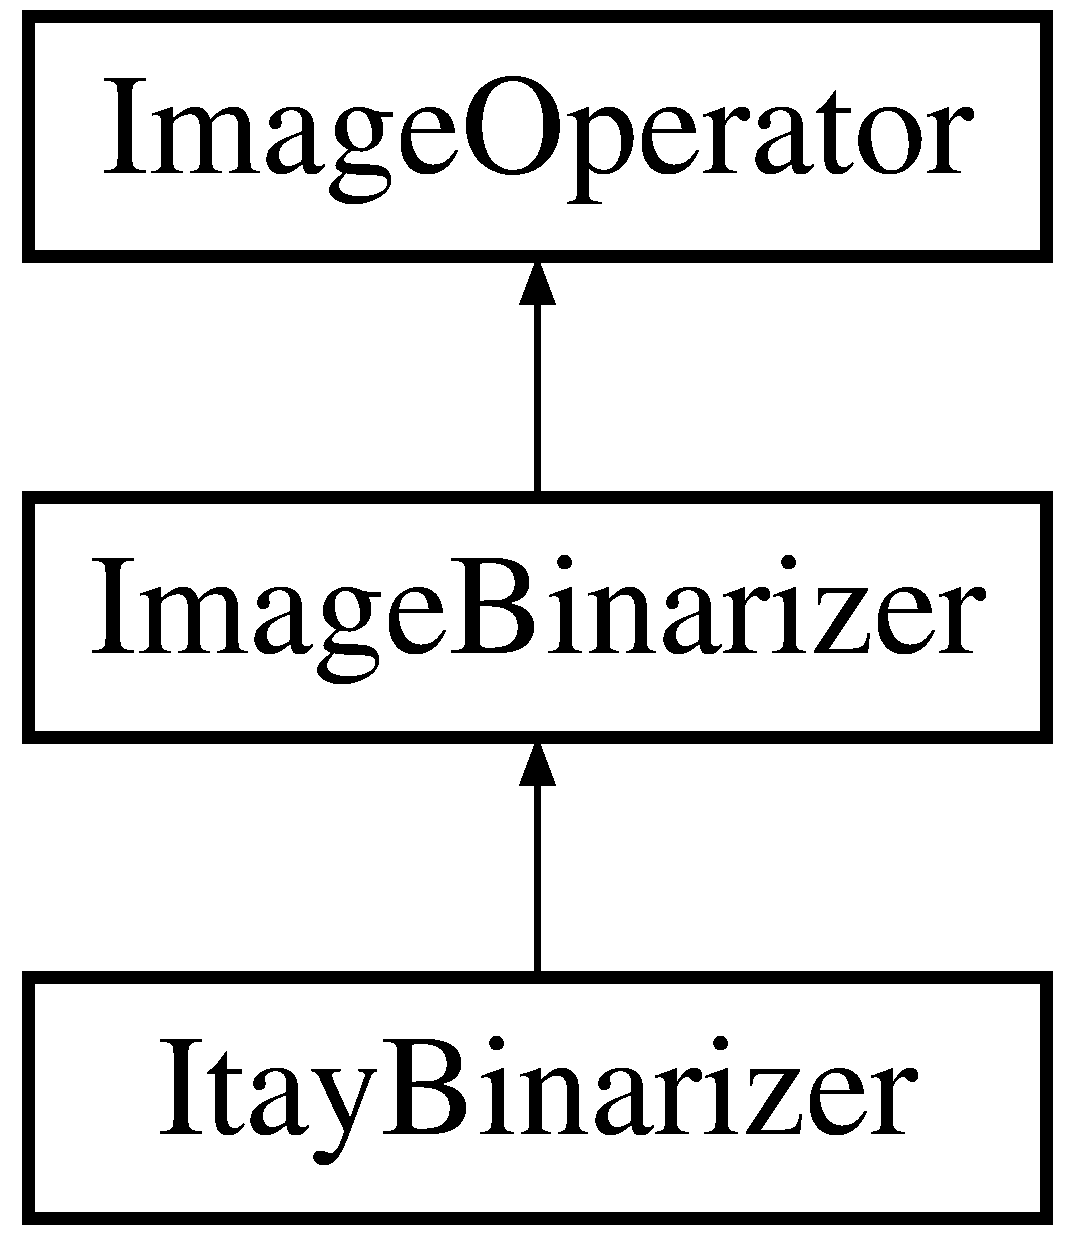
\includegraphics[height=3.000000cm]{class_itay_binarizer}
\end{center}
\end{figure}
\subsection*{Public Member Functions}
\begin{DoxyCompactItemize}
\item 
\hyperlink{class_itay_binarizer_acdebbcdfb59f5d226d85aafe9eefd0de}{Itay\+Binarizer} (void)
\item 
\hyperlink{class_itay_binarizer_ab4d858630f5efb4ee0506fe5b53d6629}{$\sim$\+Itay\+Binarizer} (void)
\item 
\hyperlink{class_d_image}{D\+Image} $\ast$ \hyperlink{class_itay_binarizer_ad0093e357fe07cc4b42dcc2f0f416832}{binarize} ()
\begin{DoxyCompactList}\small\item\em Binarize is the virtual function to implement a binarization algorithm in the extended class \end{DoxyCompactList}\end{DoxyCompactItemize}
\subsection*{Additional Inherited Members}


\subsection{Detailed Description}
Itay binarizer class implements the Itay binarization algorithm 

El Sana, 2/15/2012. 

\subsection{Constructor \& Destructor Documentation}
\hypertarget{class_itay_binarizer_acdebbcdfb59f5d226d85aafe9eefd0de}{\index{Itay\+Binarizer@{Itay\+Binarizer}!Itay\+Binarizer@{Itay\+Binarizer}}
\index{Itay\+Binarizer@{Itay\+Binarizer}!Itay\+Binarizer@{Itay\+Binarizer}}
\subsubsection[{Itay\+Binarizer}]{\setlength{\rightskip}{0pt plus 5cm}Itay\+Binarizer\+::\+Itay\+Binarizer (
\begin{DoxyParamCaption}
\item[{void}]{}
\end{DoxyParamCaption}
)}}\label{class_itay_binarizer_acdebbcdfb59f5d226d85aafe9eefd0de}
\hypertarget{class_itay_binarizer_ab4d858630f5efb4ee0506fe5b53d6629}{\index{Itay\+Binarizer@{Itay\+Binarizer}!````~Itay\+Binarizer@{$\sim$\+Itay\+Binarizer}}
\index{````~Itay\+Binarizer@{$\sim$\+Itay\+Binarizer}!Itay\+Binarizer@{Itay\+Binarizer}}
\subsubsection[{$\sim$\+Itay\+Binarizer}]{\setlength{\rightskip}{0pt plus 5cm}Itay\+Binarizer\+::$\sim$\+Itay\+Binarizer (
\begin{DoxyParamCaption}
\item[{void}]{}
\end{DoxyParamCaption}
)}}\label{class_itay_binarizer_ab4d858630f5efb4ee0506fe5b53d6629}


\subsection{Member Function Documentation}
\hypertarget{class_itay_binarizer_ad0093e357fe07cc4b42dcc2f0f416832}{\index{Itay\+Binarizer@{Itay\+Binarizer}!binarize@{binarize}}
\index{binarize@{binarize}!Itay\+Binarizer@{Itay\+Binarizer}}
\subsubsection[{binarize}]{\setlength{\rightskip}{0pt plus 5cm}{\bf D\+Image} $\ast$ Itay\+Binarizer\+::binarize (
\begin{DoxyParamCaption}
{}
\end{DoxyParamCaption}
)\hspace{0.3cm}{\ttfamily [virtual]}}}\label{class_itay_binarizer_ad0093e357fe07cc4b42dcc2f0f416832}


Binarize is the virtual function to implement a binarization algorithm in the extended class 

El Sana, 2/15/2012. 

\begin{DoxyReturn}{Returns}
null if it fails, else. 
\end{DoxyReturn}


Implements \hyperlink{class_image_binarizer_accf059357ade25887a94c91f76262254}{Image\+Binarizer}.



The documentation for this class was generated from the following files\+:\begin{DoxyCompactItemize}
\item 
Manuscript\+App/\hyperlink{_itay_binarizer_8h}{Itay\+Binarizer.\+h}\item 
Manuscript\+App/\hyperlink{_itay_binarizer_8cpp}{Itay\+Binarizer.\+cpp}\end{DoxyCompactItemize}

\hypertarget{class_metric}{\section{Metric Class Reference}
\label{class_metric}\index{Metric@{Metric}}
}


{\ttfamily \#include $<$Metric.\+h$>$}

Inheritance diagram for Metric\+:\begin{figure}[H]
\begin{center}
\leavevmode
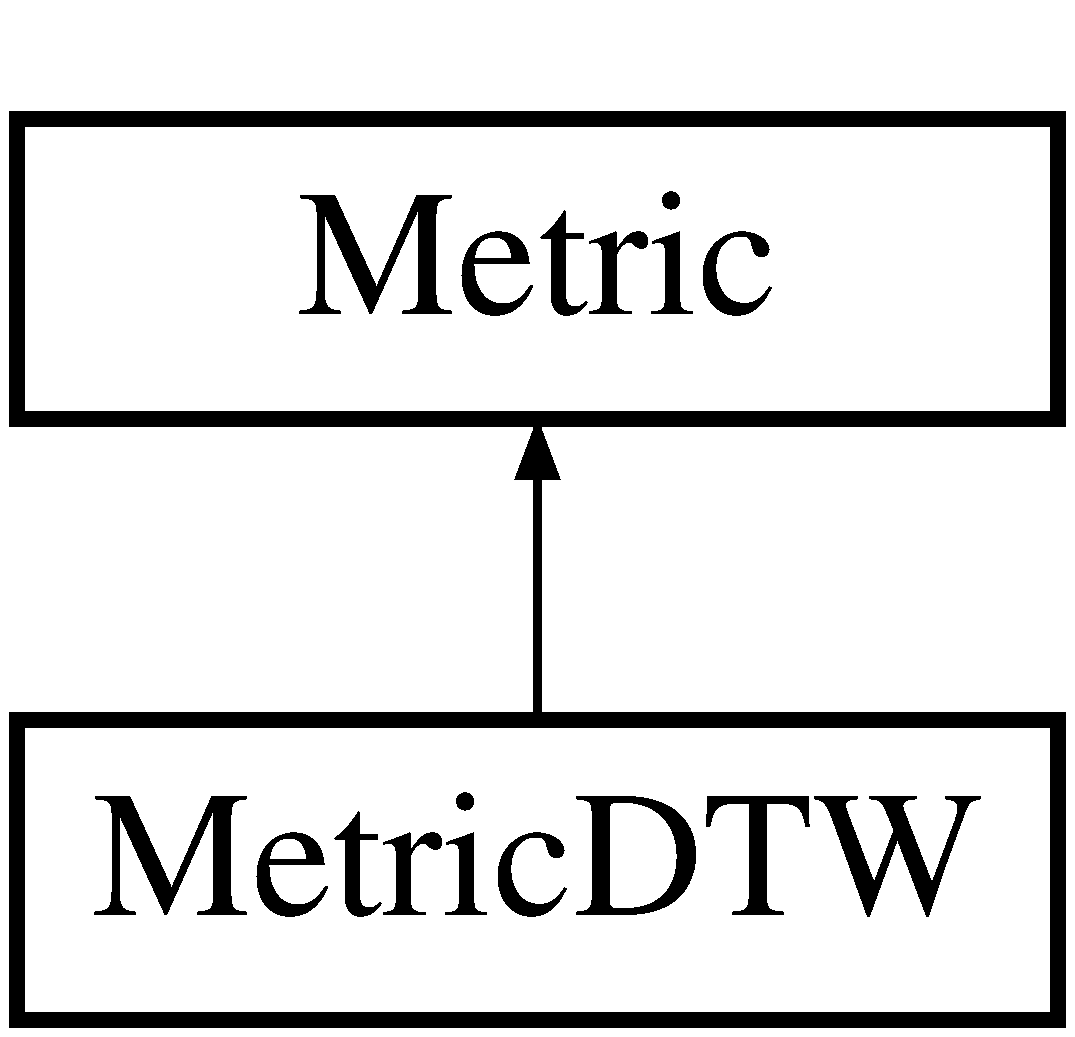
\includegraphics[height=2.000000cm]{class_metric}
\end{center}
\end{figure}
\subsection*{Public Member Functions}
\begin{DoxyCompactItemize}
\item 
\hyperlink{class_metric_ade0443abd5c6080f406288ee650b416b}{Metric} (void)
\item 
\hyperlink{class_metric_a68ec53fa39cba9520dd20dceab1668fa}{$\sim$\+Metric} (void)
\item 
virtual double \hyperlink{class_metric_a0609682cc98cbd0a5e94df800ff18145}{distance} (\hyperlink{class_feature}{Feature} $\ast$a, \hyperlink{class_feature}{Feature} $\ast$b)=0
\item 
virtual double \hyperlink{class_metric_aeffee7c23f39f51669c4ce8cd7551cdd}{distance} (vector$<$ \hyperlink{class_feature}{Feature} $\ast$ $>$ \&a, vector$<$ \hyperlink{class_feature}{Feature} $\ast$ $>$ \&b)=0
\end{DoxyCompactItemize}


\subsection{Constructor \& Destructor Documentation}
\hypertarget{class_metric_ade0443abd5c6080f406288ee650b416b}{\index{Metric@{Metric}!Metric@{Metric}}
\index{Metric@{Metric}!Metric@{Metric}}
\subsubsection[{Metric}]{\setlength{\rightskip}{0pt plus 5cm}Metric\+::\+Metric (
\begin{DoxyParamCaption}
\item[{void}]{}
\end{DoxyParamCaption}
)\hspace{0.3cm}{\ttfamily [inline]}}}\label{class_metric_ade0443abd5c6080f406288ee650b416b}
\hypertarget{class_metric_a68ec53fa39cba9520dd20dceab1668fa}{\index{Metric@{Metric}!````~Metric@{$\sim$\+Metric}}
\index{````~Metric@{$\sim$\+Metric}!Metric@{Metric}}
\subsubsection[{$\sim$\+Metric}]{\setlength{\rightskip}{0pt plus 5cm}Metric\+::$\sim$\+Metric (
\begin{DoxyParamCaption}
\item[{void}]{}
\end{DoxyParamCaption}
)\hspace{0.3cm}{\ttfamily [inline]}}}\label{class_metric_a68ec53fa39cba9520dd20dceab1668fa}


\subsection{Member Function Documentation}
\hypertarget{class_metric_a0609682cc98cbd0a5e94df800ff18145}{\index{Metric@{Metric}!distance@{distance}}
\index{distance@{distance}!Metric@{Metric}}
\subsubsection[{distance}]{\setlength{\rightskip}{0pt plus 5cm}virtual double Metric\+::distance (
\begin{DoxyParamCaption}
\item[{{\bf Feature} $\ast$}]{a, }
\item[{{\bf Feature} $\ast$}]{b}
\end{DoxyParamCaption}
)\hspace{0.3cm}{\ttfamily [pure virtual]}}}\label{class_metric_a0609682cc98cbd0a5e94df800ff18145}


Implemented in \hyperlink{class_metric_d_t_w_a39e2011060167764d3c7e65e5072fbb5}{Metric\+D\+T\+W}.

\hypertarget{class_metric_aeffee7c23f39f51669c4ce8cd7551cdd}{\index{Metric@{Metric}!distance@{distance}}
\index{distance@{distance}!Metric@{Metric}}
\subsubsection[{distance}]{\setlength{\rightskip}{0pt plus 5cm}virtual double Metric\+::distance (
\begin{DoxyParamCaption}
\item[{vector$<$ {\bf Feature} $\ast$ $>$ \&}]{a, }
\item[{vector$<$ {\bf Feature} $\ast$ $>$ \&}]{b}
\end{DoxyParamCaption}
)\hspace{0.3cm}{\ttfamily [pure virtual]}}}\label{class_metric_aeffee7c23f39f51669c4ce8cd7551cdd}


Implemented in \hyperlink{class_metric_d_t_w_a7343dcb7bd4d654959e12bfb672622a2}{Metric\+D\+T\+W}.



The documentation for this class was generated from the following file\+:\begin{DoxyCompactItemize}
\item 
Manuscript\+App/\hyperlink{_metric_8h}{Metric.\+h}\end{DoxyCompactItemize}

\hypertarget{class_metric_d_t_w}{\section{Metric\+D\+T\+W Class Reference}
\label{class_metric_d_t_w}\index{Metric\+D\+T\+W@{Metric\+D\+T\+W}}
}


{\ttfamily \#include $<$Metric\+D\+T\+W.\+h$>$}

Inheritance diagram for Metric\+D\+T\+W\+:\begin{figure}[H]
\begin{center}
\leavevmode
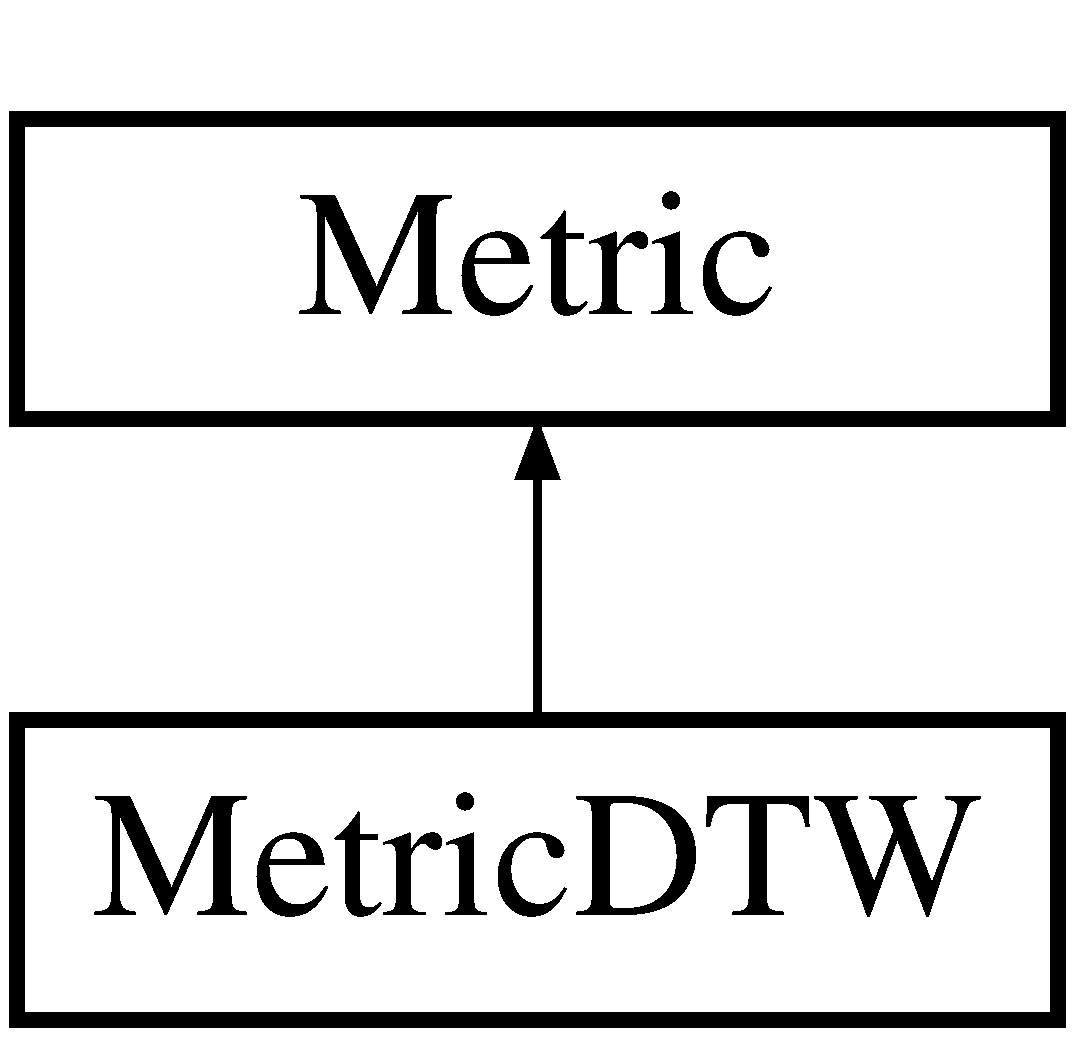
\includegraphics[height=2.000000cm]{class_metric_d_t_w}
\end{center}
\end{figure}
\subsection*{Public Member Functions}
\begin{DoxyCompactItemize}
\item 
\hyperlink{class_metric_d_t_w_af3d7712e07808d281e8884432db40cf0}{Metric\+D\+T\+W} (void)
\item 
\hyperlink{class_metric_d_t_w_a1a84f60596f8517bb360f362e82b277a}{$\sim$\+Metric\+D\+T\+W} (void)
\item 
void \hyperlink{class_metric_d_t_w_ae10fb8483b49695918429f3cb960a063}{init\+Distance\+Map} (vector$<$ \hyperlink{class_feature}{Feature} $\ast$ $>$ \&a, vector$<$ \hyperlink{class_feature}{Feature} $\ast$ $>$ \&b)
\item 
double \hyperlink{class_metric_d_t_w_a39e2011060167764d3c7e65e5072fbb5}{distance} (\hyperlink{class_feature}{Feature} $\ast$a, \hyperlink{class_feature}{Feature} $\ast$b)
\item 
double \hyperlink{class_metric_d_t_w_a7343dcb7bd4d654959e12bfb672622a2}{distance} (vector$<$ \hyperlink{class_feature}{Feature} $\ast$ $>$ \&a, vector$<$ \hyperlink{class_feature}{Feature} $\ast$ $>$ \&b)
\item 
void \hyperlink{class_metric_d_t_w_a37af163866e5922fccc8676ca236a6f2}{find\+Minimal\+Path} (vector$<$ cv\+::\+Point2i $>$ \&path)
\item 
double \hyperlink{class_metric_d_t_w_addd6e64c5742481e13bccf48daf62248}{distance\+From\+Diagonal} (vector$<$ cv\+::\+Point2i $>$ \&path)
\item 
void \hyperlink{class_metric_d_t_w_ac5a4922e152fad12a7e91ab5884b4e86}{print} (vector$<$ cv\+::\+Point2i $>$ \&path)
\end{DoxyCompactItemize}


\subsection{Constructor \& Destructor Documentation}
\hypertarget{class_metric_d_t_w_af3d7712e07808d281e8884432db40cf0}{\index{Metric\+D\+T\+W@{Metric\+D\+T\+W}!Metric\+D\+T\+W@{Metric\+D\+T\+W}}
\index{Metric\+D\+T\+W@{Metric\+D\+T\+W}!Metric\+D\+T\+W@{Metric\+D\+T\+W}}
\subsubsection[{Metric\+D\+T\+W}]{\setlength{\rightskip}{0pt plus 5cm}Metric\+D\+T\+W\+::\+Metric\+D\+T\+W (
\begin{DoxyParamCaption}
\item[{void}]{}
\end{DoxyParamCaption}
)\hspace{0.3cm}{\ttfamily [inline]}}}\label{class_metric_d_t_w_af3d7712e07808d281e8884432db40cf0}
\hypertarget{class_metric_d_t_w_a1a84f60596f8517bb360f362e82b277a}{\index{Metric\+D\+T\+W@{Metric\+D\+T\+W}!````~Metric\+D\+T\+W@{$\sim$\+Metric\+D\+T\+W}}
\index{````~Metric\+D\+T\+W@{$\sim$\+Metric\+D\+T\+W}!Metric\+D\+T\+W@{Metric\+D\+T\+W}}
\subsubsection[{$\sim$\+Metric\+D\+T\+W}]{\setlength{\rightskip}{0pt plus 5cm}Metric\+D\+T\+W\+::$\sim$\+Metric\+D\+T\+W (
\begin{DoxyParamCaption}
\item[{void}]{}
\end{DoxyParamCaption}
)\hspace{0.3cm}{\ttfamily [inline]}}}\label{class_metric_d_t_w_a1a84f60596f8517bb360f362e82b277a}


\subsection{Member Function Documentation}
\hypertarget{class_metric_d_t_w_a39e2011060167764d3c7e65e5072fbb5}{\index{Metric\+D\+T\+W@{Metric\+D\+T\+W}!distance@{distance}}
\index{distance@{distance}!Metric\+D\+T\+W@{Metric\+D\+T\+W}}
\subsubsection[{distance}]{\setlength{\rightskip}{0pt plus 5cm}double Metric\+D\+T\+W\+::distance (
\begin{DoxyParamCaption}
\item[{{\bf Feature} $\ast$}]{a, }
\item[{{\bf Feature} $\ast$}]{b}
\end{DoxyParamCaption}
)\hspace{0.3cm}{\ttfamily [virtual]}}}\label{class_metric_d_t_w_a39e2011060167764d3c7e65e5072fbb5}


Implements \hyperlink{class_metric_a0609682cc98cbd0a5e94df800ff18145}{Metric}.

\hypertarget{class_metric_d_t_w_a7343dcb7bd4d654959e12bfb672622a2}{\index{Metric\+D\+T\+W@{Metric\+D\+T\+W}!distance@{distance}}
\index{distance@{distance}!Metric\+D\+T\+W@{Metric\+D\+T\+W}}
\subsubsection[{distance}]{\setlength{\rightskip}{0pt plus 5cm}double Metric\+D\+T\+W\+::distance (
\begin{DoxyParamCaption}
\item[{vector$<$ {\bf Feature} $\ast$ $>$ \&}]{a, }
\item[{vector$<$ {\bf Feature} $\ast$ $>$ \&}]{b}
\end{DoxyParamCaption}
)\hspace{0.3cm}{\ttfamily [virtual]}}}\label{class_metric_d_t_w_a7343dcb7bd4d654959e12bfb672622a2}


Implements \hyperlink{class_metric_aeffee7c23f39f51669c4ce8cd7551cdd}{Metric}.

\hypertarget{class_metric_d_t_w_addd6e64c5742481e13bccf48daf62248}{\index{Metric\+D\+T\+W@{Metric\+D\+T\+W}!distance\+From\+Diagonal@{distance\+From\+Diagonal}}
\index{distance\+From\+Diagonal@{distance\+From\+Diagonal}!Metric\+D\+T\+W@{Metric\+D\+T\+W}}
\subsubsection[{distance\+From\+Diagonal}]{\setlength{\rightskip}{0pt plus 5cm}double Metric\+D\+T\+W\+::distance\+From\+Diagonal (
\begin{DoxyParamCaption}
\item[{vector$<$ cv\+::\+Point2i $>$ \&}]{path}
\end{DoxyParamCaption}
)}}\label{class_metric_d_t_w_addd6e64c5742481e13bccf48daf62248}
\hypertarget{class_metric_d_t_w_a37af163866e5922fccc8676ca236a6f2}{\index{Metric\+D\+T\+W@{Metric\+D\+T\+W}!find\+Minimal\+Path@{find\+Minimal\+Path}}
\index{find\+Minimal\+Path@{find\+Minimal\+Path}!Metric\+D\+T\+W@{Metric\+D\+T\+W}}
\subsubsection[{find\+Minimal\+Path}]{\setlength{\rightskip}{0pt plus 5cm}void Metric\+D\+T\+W\+::find\+Minimal\+Path (
\begin{DoxyParamCaption}
\item[{vector$<$ cv\+::\+Point2i $>$ \&}]{path}
\end{DoxyParamCaption}
)}}\label{class_metric_d_t_w_a37af163866e5922fccc8676ca236a6f2}
\hypertarget{class_metric_d_t_w_ae10fb8483b49695918429f3cb960a063}{\index{Metric\+D\+T\+W@{Metric\+D\+T\+W}!init\+Distance\+Map@{init\+Distance\+Map}}
\index{init\+Distance\+Map@{init\+Distance\+Map}!Metric\+D\+T\+W@{Metric\+D\+T\+W}}
\subsubsection[{init\+Distance\+Map}]{\setlength{\rightskip}{0pt plus 5cm}void Metric\+D\+T\+W\+::init\+Distance\+Map (
\begin{DoxyParamCaption}
\item[{vector$<$ {\bf Feature} $\ast$ $>$ \&}]{a, }
\item[{vector$<$ {\bf Feature} $\ast$ $>$ \&}]{b}
\end{DoxyParamCaption}
)}}\label{class_metric_d_t_w_ae10fb8483b49695918429f3cb960a063}
\hypertarget{class_metric_d_t_w_ac5a4922e152fad12a7e91ab5884b4e86}{\index{Metric\+D\+T\+W@{Metric\+D\+T\+W}!print@{print}}
\index{print@{print}!Metric\+D\+T\+W@{Metric\+D\+T\+W}}
\subsubsection[{print}]{\setlength{\rightskip}{0pt plus 5cm}void Metric\+D\+T\+W\+::print (
\begin{DoxyParamCaption}
\item[{vector$<$ cv\+::\+Point2i $>$ \&}]{path}
\end{DoxyParamCaption}
)}}\label{class_metric_d_t_w_ac5a4922e152fad12a7e91ab5884b4e86}


The documentation for this class was generated from the following files\+:\begin{DoxyCompactItemize}
\item 
Manuscript\+App/\hyperlink{_metric_d_t_w_8h}{Metric\+D\+T\+W.\+h}\item 
Manuscript\+App/\hyperlink{_metric_d_t_w_8cpp}{Metric\+D\+T\+W.\+cpp}\end{DoxyCompactItemize}

\hypertarget{class_otsu_binarizer}{\section{Otsu\+Binarizer Class Reference}
\label{class_otsu_binarizer}\index{Otsu\+Binarizer@{Otsu\+Binarizer}}
}


Otsul binarizer class implements the Otsu binarization algorithm  




{\ttfamily \#include $<$Otsu\+Binarizer.\+h$>$}

Inheritance diagram for Otsu\+Binarizer\+:\begin{figure}[H]
\begin{center}
\leavevmode
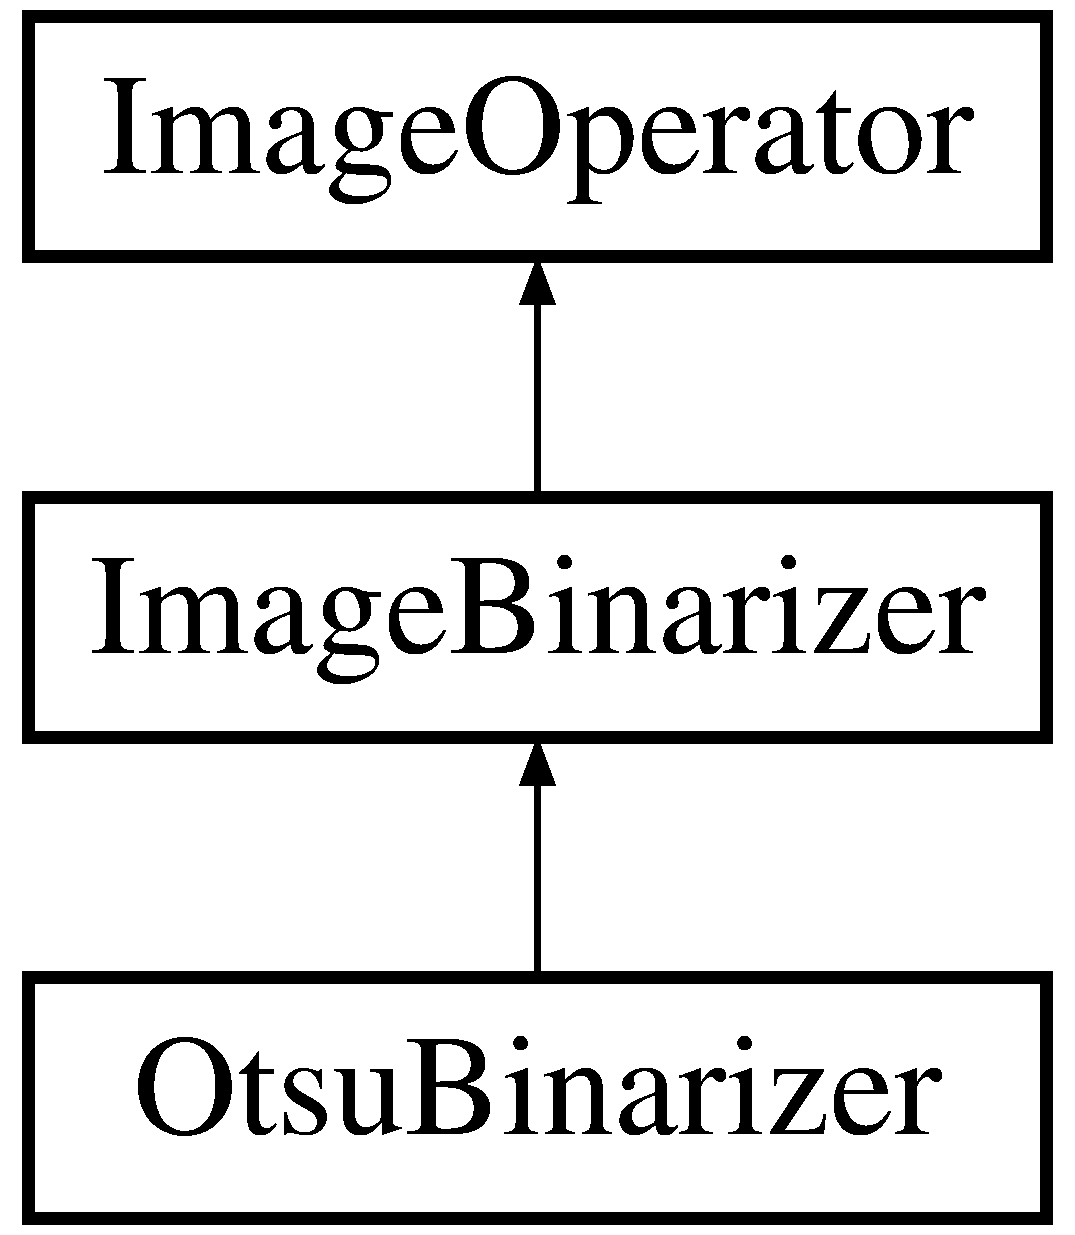
\includegraphics[height=3.000000cm]{class_otsu_binarizer}
\end{center}
\end{figure}
\subsection*{Public Member Functions}
\begin{DoxyCompactItemize}
\item 
\hyperlink{class_d_image}{D\+Image} $\ast$ \hyperlink{class_otsu_binarizer_a4219a9f9e72d1d0eceee30402bf2afd5}{binarize} ()
\begin{DoxyCompactList}\small\item\em binarize an image using the Otsu algorithm \end{DoxyCompactList}\end{DoxyCompactItemize}
\subsection*{Additional Inherited Members}


\subsection{Detailed Description}
Otsul binarizer class implements the Otsu binarization algorithm 

El Sana, 2/15/2012. 

\subsection{Member Function Documentation}
\hypertarget{class_otsu_binarizer_a4219a9f9e72d1d0eceee30402bf2afd5}{\index{Otsu\+Binarizer@{Otsu\+Binarizer}!binarize@{binarize}}
\index{binarize@{binarize}!Otsu\+Binarizer@{Otsu\+Binarizer}}
\subsubsection[{binarize}]{\setlength{\rightskip}{0pt plus 5cm}{\bf D\+Image} $\ast$ Otsu\+Binarizer\+::binarize (
\begin{DoxyParamCaption}
{}
\end{DoxyParamCaption}
)\hspace{0.3cm}{\ttfamily [virtual]}}}\label{class_otsu_binarizer_a4219a9f9e72d1d0eceee30402bf2afd5}


binarize an image using the Otsu algorithm 

El Sana, 2/15/2012. 

\begin{DoxyReturn}{Returns}
null if it fails, else. 
\end{DoxyReturn}


Implements \hyperlink{class_image_binarizer_accf059357ade25887a94c91f76262254}{Image\+Binarizer}.



The documentation for this class was generated from the following files\+:\begin{DoxyCompactItemize}
\item 
Manuscript\+App/\hyperlink{_otsu_binarizer_8h}{Otsu\+Binarizer.\+h}\item 
Manuscript\+App/\hyperlink{_otsu_binarizer_8cpp}{Otsu\+Binarizer.\+cpp}\end{DoxyCompactItemize}

\hypertarget{class_otsul_binarizer}{\section{Otsul\+Binarizer Class Reference}
\label{class_otsul_binarizer}\index{Otsul\+Binarizer@{Otsul\+Binarizer}}
}


Otsul binarizer class implements the Otsu binarization algorithm  




{\ttfamily \#include $<$Otsul\+Binarizer.\+h$>$}

Inheritance diagram for Otsul\+Binarizer\+:\begin{figure}[H]
\begin{center}
\leavevmode
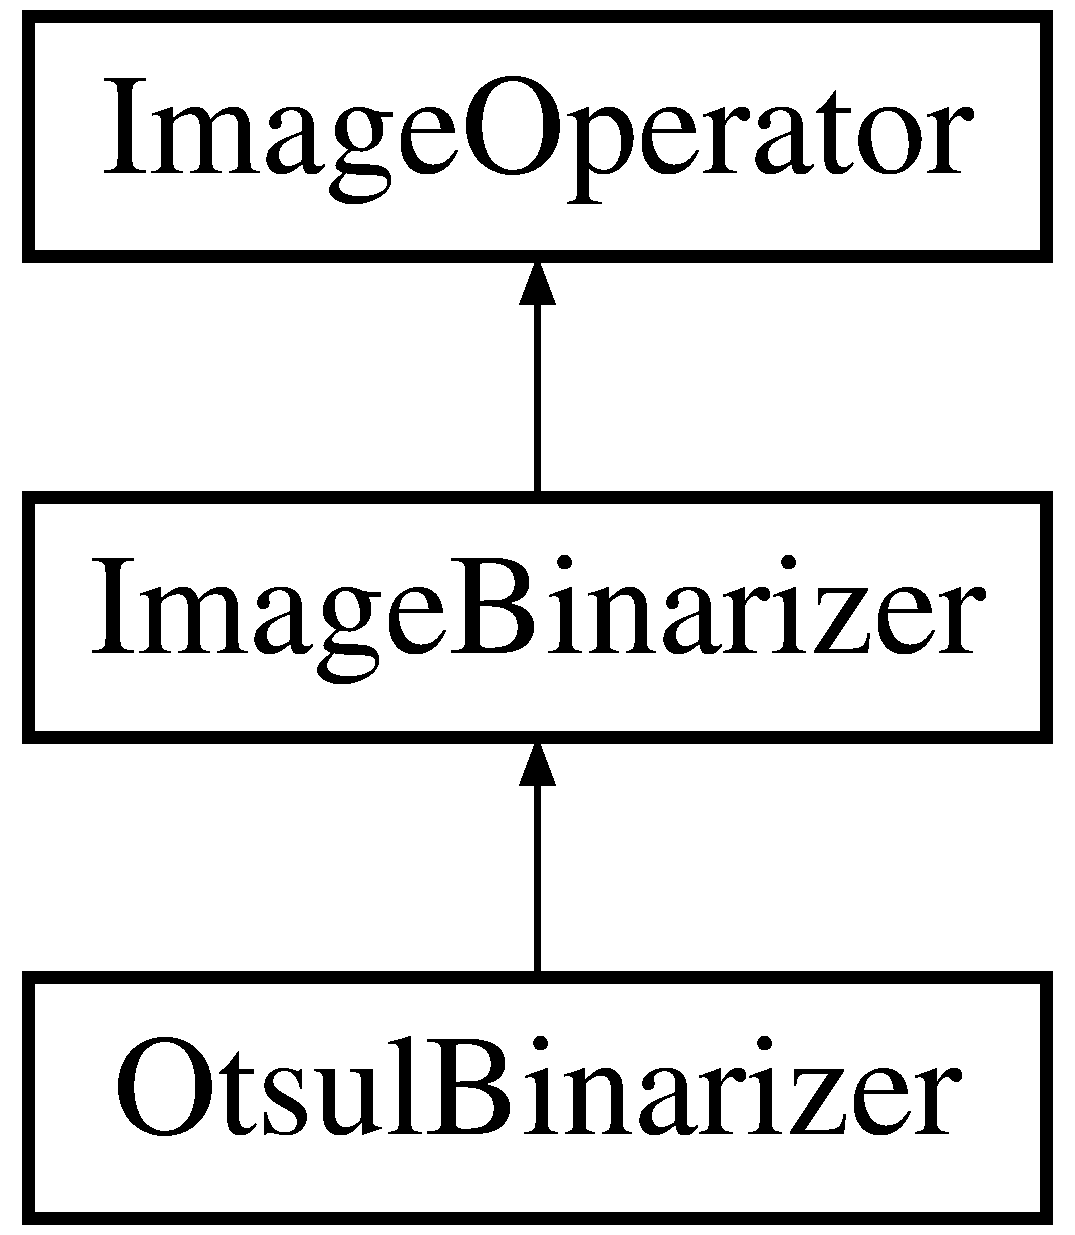
\includegraphics[height=3.000000cm]{class_otsul_binarizer}
\end{center}
\end{figure}
\subsection*{Public Member Functions}
\begin{DoxyCompactItemize}
\item 
\hyperlink{class_d_image}{D\+Image} $\ast$ \hyperlink{class_otsul_binarizer_a14064c86e424c1e68625b7fbc07195d5}{binarize} ()
\begin{DoxyCompactList}\small\item\em binarize an image using the Otsu algorithm \end{DoxyCompactList}\end{DoxyCompactItemize}
\subsection*{Additional Inherited Members}


\subsection{Detailed Description}
Otsul binarizer class implements the Otsu binarization algorithm 

El Sana, 2/15/2012. 

\subsection{Member Function Documentation}
\hypertarget{class_otsul_binarizer_a14064c86e424c1e68625b7fbc07195d5}{\index{Otsul\+Binarizer@{Otsul\+Binarizer}!binarize@{binarize}}
\index{binarize@{binarize}!Otsul\+Binarizer@{Otsul\+Binarizer}}
\subsubsection[{binarize}]{\setlength{\rightskip}{0pt plus 5cm}{\bf D\+Image} $\ast$ Otsul\+Binarizer\+::binarize (
\begin{DoxyParamCaption}
{}
\end{DoxyParamCaption}
)\hspace{0.3cm}{\ttfamily [virtual]}}}\label{class_otsul_binarizer_a14064c86e424c1e68625b7fbc07195d5}


binarize an image using the Otsu algorithm 

El Sana, 2/15/2012. 

\begin{DoxyReturn}{Returns}
null if it fails, else. 
\end{DoxyReturn}


Implements \hyperlink{class_image_binarizer_accf059357ade25887a94c91f76262254}{Image\+Binarizer}.



The documentation for this class was generated from the following files\+:\begin{DoxyCompactItemize}
\item 
Manuscript\+App/\hyperlink{_otsul_binarizer_8h}{Otsul\+Binarizer.\+h}\item 
Manuscript\+App/\hyperlink{_otsul_binarizer_8cpp}{Otsul\+Binarizer.\+cpp}\end{DoxyCompactItemize}

\hypertarget{class_page_image}{\section{Page\+Image Class Reference}
\label{class_page_image}\index{Page\+Image@{Page\+Image}}
}


{\ttfamily \#include $<$Page\+Image.\+h$>$}

Inheritance diagram for Page\+Image\+:\begin{figure}[H]
\begin{center}
\leavevmode
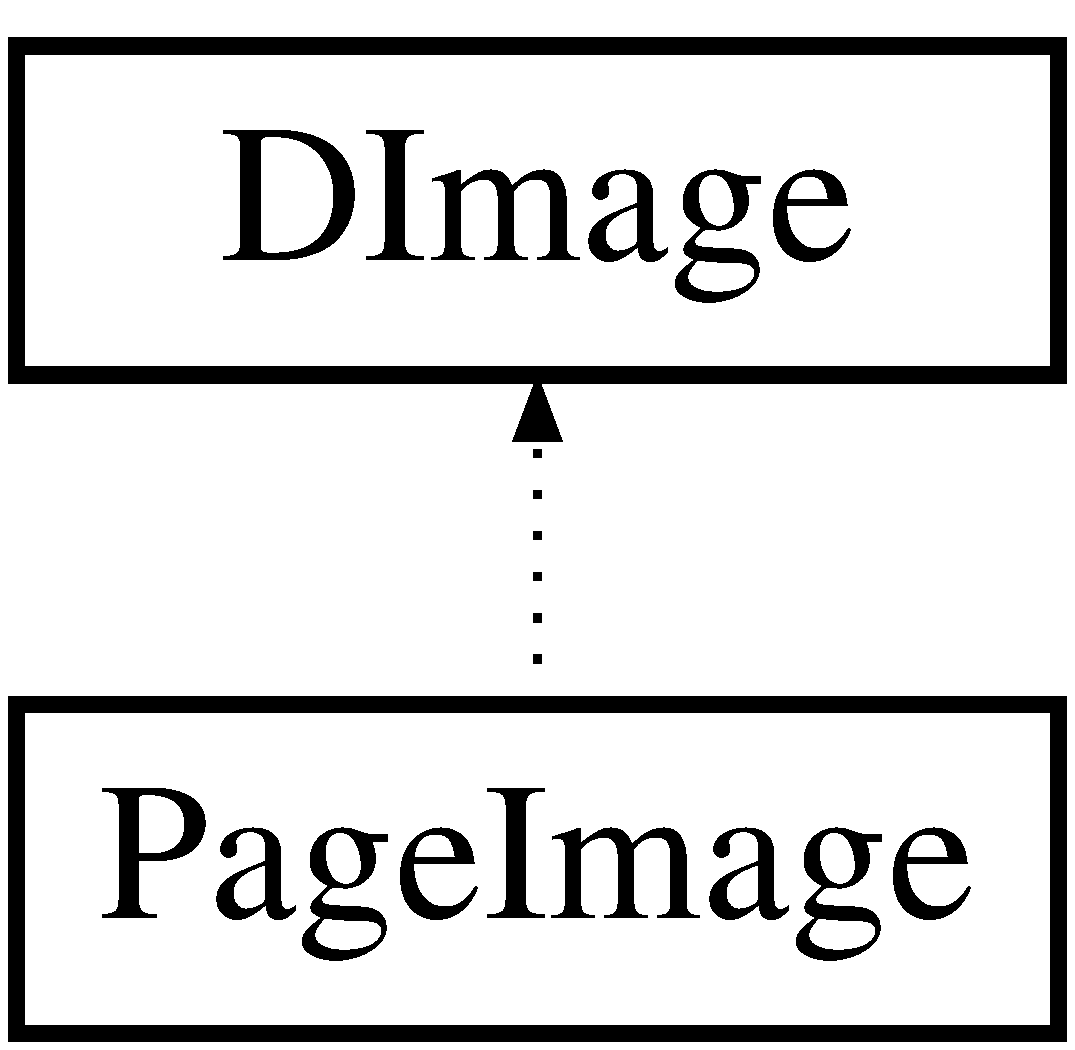
\includegraphics[height=2.000000cm]{class_page_image}
\end{center}
\end{figure}
\subsection*{Public Member Functions}
\begin{DoxyCompactItemize}
\item 
\hyperlink{class_page_image_acd6291149a801930fe85801780a480a1}{Page\+Image} (void)
\item 
\hyperlink{class_page_image_a3a5b95965ac1d84f71c5ba3ee4890558}{$\sim$\+Page\+Image} (void)
\item 
void \hyperlink{class_page_image_a8fb57e9c831783972f64a1befe0eb108}{set\+Main\+Fragment} (\hyperlink{class_d_image}{D\+Image} $\ast$dimg)
\item 
\hyperlink{class_d_image}{D\+Image} $\ast$ \hyperlink{class_page_image_ae865d0cb7d4c1f51ed70180bd2e9894f}{get\+Main\+Fragment} ()
\item 
void \hyperlink{class_page_image_aa06ea24ceaca41d73bb12062a5c806eb}{add\+Margin\+Note} (\hyperlink{class_d_image}{D\+Image} $\ast$dimg)
\item 
void \hyperlink{class_page_image_a8c59ffb28ca315cef488b54bd4901f7c}{extract\+Margin\+Notes} ()
\end{DoxyCompactItemize}


\subsection{Constructor \& Destructor Documentation}
\hypertarget{class_page_image_acd6291149a801930fe85801780a480a1}{\index{Page\+Image@{Page\+Image}!Page\+Image@{Page\+Image}}
\index{Page\+Image@{Page\+Image}!Page\+Image@{Page\+Image}}
\subsubsection[{Page\+Image}]{\setlength{\rightskip}{0pt plus 5cm}Page\+Image\+::\+Page\+Image (
\begin{DoxyParamCaption}
\item[{void}]{}
\end{DoxyParamCaption}
)}}\label{class_page_image_acd6291149a801930fe85801780a480a1}
\hypertarget{class_page_image_a3a5b95965ac1d84f71c5ba3ee4890558}{\index{Page\+Image@{Page\+Image}!````~Page\+Image@{$\sim$\+Page\+Image}}
\index{````~Page\+Image@{$\sim$\+Page\+Image}!Page\+Image@{Page\+Image}}
\subsubsection[{$\sim$\+Page\+Image}]{\setlength{\rightskip}{0pt plus 5cm}Page\+Image\+::$\sim$\+Page\+Image (
\begin{DoxyParamCaption}
\item[{void}]{}
\end{DoxyParamCaption}
)}}\label{class_page_image_a3a5b95965ac1d84f71c5ba3ee4890558}


\subsection{Member Function Documentation}
\hypertarget{class_page_image_aa06ea24ceaca41d73bb12062a5c806eb}{\index{Page\+Image@{Page\+Image}!add\+Margin\+Note@{add\+Margin\+Note}}
\index{add\+Margin\+Note@{add\+Margin\+Note}!Page\+Image@{Page\+Image}}
\subsubsection[{add\+Margin\+Note}]{\setlength{\rightskip}{0pt plus 5cm}void Page\+Image\+::add\+Margin\+Note (
\begin{DoxyParamCaption}
\item[{{\bf D\+Image} $\ast$}]{dimg}
\end{DoxyParamCaption}
)\hspace{0.3cm}{\ttfamily [inline]}}}\label{class_page_image_aa06ea24ceaca41d73bb12062a5c806eb}
\hypertarget{class_page_image_a8c59ffb28ca315cef488b54bd4901f7c}{\index{Page\+Image@{Page\+Image}!extract\+Margin\+Notes@{extract\+Margin\+Notes}}
\index{extract\+Margin\+Notes@{extract\+Margin\+Notes}!Page\+Image@{Page\+Image}}
\subsubsection[{extract\+Margin\+Notes}]{\setlength{\rightskip}{0pt plus 5cm}void Page\+Image\+::extract\+Margin\+Notes (
\begin{DoxyParamCaption}
{}
\end{DoxyParamCaption}
)}}\label{class_page_image_a8c59ffb28ca315cef488b54bd4901f7c}
\hypertarget{class_page_image_ae865d0cb7d4c1f51ed70180bd2e9894f}{\index{Page\+Image@{Page\+Image}!get\+Main\+Fragment@{get\+Main\+Fragment}}
\index{get\+Main\+Fragment@{get\+Main\+Fragment}!Page\+Image@{Page\+Image}}
\subsubsection[{get\+Main\+Fragment}]{\setlength{\rightskip}{0pt plus 5cm}{\bf D\+Image}$\ast$ Page\+Image\+::get\+Main\+Fragment (
\begin{DoxyParamCaption}
{}
\end{DoxyParamCaption}
)\hspace{0.3cm}{\ttfamily [inline]}}}\label{class_page_image_ae865d0cb7d4c1f51ed70180bd2e9894f}
\hypertarget{class_page_image_a8fb57e9c831783972f64a1befe0eb108}{\index{Page\+Image@{Page\+Image}!set\+Main\+Fragment@{set\+Main\+Fragment}}
\index{set\+Main\+Fragment@{set\+Main\+Fragment}!Page\+Image@{Page\+Image}}
\subsubsection[{set\+Main\+Fragment}]{\setlength{\rightskip}{0pt plus 5cm}void Page\+Image\+::set\+Main\+Fragment (
\begin{DoxyParamCaption}
\item[{{\bf D\+Image} $\ast$}]{dimg}
\end{DoxyParamCaption}
)\hspace{0.3cm}{\ttfamily [inline]}}}\label{class_page_image_a8fb57e9c831783972f64a1befe0eb108}


The documentation for this class was generated from the following files\+:\begin{DoxyCompactItemize}
\item 
Manuscript\+App/\hyperlink{_page_image_8h}{Page\+Image.\+h}\item 
Manuscript\+App/\hyperlink{_page_image_8cpp}{Page\+Image.\+cpp}\end{DoxyCompactItemize}

\hypertarget{class_profile_seam_text_line_extractor}{\section{Profile\+Seam\+Text\+Line\+Extractor Class Reference}
\label{class_profile_seam_text_line_extractor}\index{Profile\+Seam\+Text\+Line\+Extractor@{Profile\+Seam\+Text\+Line\+Extractor}}
}


{\ttfamily \#include $<$Profile\+Seam\+Text\+Line\+Extractor.\+h$>$}

Inheritance diagram for Profile\+Seam\+Text\+Line\+Extractor\+:\begin{figure}[H]
\begin{center}
\leavevmode
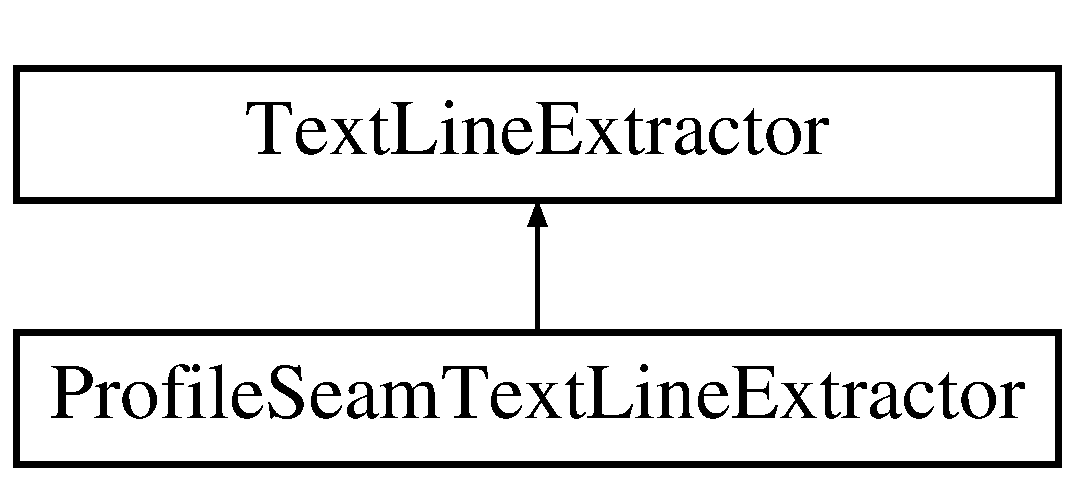
\includegraphics[height=2.000000cm]{class_profile_seam_text_line_extractor}
\end{center}
\end{figure}
\subsection*{Public Member Functions}
\begin{DoxyCompactItemize}
\item 
vector$<$ vector$<$ int $>$ $>$ \hyperlink{class_profile_seam_text_line_extractor_a8221b34c948ac11481e2b8c8658ca4c6}{compute\+Seperating\+Seams} ()
\item 
void \hyperlink{class_profile_seam_text_line_extractor_adf05463fd596d059da9669d3f8e43fed}{Medial\+Seam\+Drawing} ()
\item 
\hyperlink{class_profile_seam_text_line_extractor_ab20c9e4368b7f767e14dc96715bb6567}{Profile\+Seam\+Text\+Line\+Extractor} (\hyperlink{class_projection_profile}{Projection\+Profile} proj, \hyperlink{class_d_image}{D\+Image} $\ast$prof, Mat img)
\item 
\hyperlink{class_profile_seam_text_line_extractor_a96e8293704190d08a00afb7fc0127f98}{$\sim$\+Profile\+Seam\+Text\+Line\+Extractor} ()
\item 
void \hyperlink{class_profile_seam_text_line_extractor_a67017476e961c0531524d3f52cf70e23}{extract} ()
\end{DoxyCompactItemize}
\subsection*{Additional Inherited Members}


\subsection{Constructor \& Destructor Documentation}
\hypertarget{class_profile_seam_text_line_extractor_ab20c9e4368b7f767e14dc96715bb6567}{\index{Profile\+Seam\+Text\+Line\+Extractor@{Profile\+Seam\+Text\+Line\+Extractor}!Profile\+Seam\+Text\+Line\+Extractor@{Profile\+Seam\+Text\+Line\+Extractor}}
\index{Profile\+Seam\+Text\+Line\+Extractor@{Profile\+Seam\+Text\+Line\+Extractor}!Profile\+Seam\+Text\+Line\+Extractor@{Profile\+Seam\+Text\+Line\+Extractor}}
\subsubsection[{Profile\+Seam\+Text\+Line\+Extractor}]{\setlength{\rightskip}{0pt plus 5cm}Profile\+Seam\+Text\+Line\+Extractor\+::\+Profile\+Seam\+Text\+Line\+Extractor (
\begin{DoxyParamCaption}
\item[{{\bf Projection\+Profile}}]{proj, }
\item[{{\bf D\+Image} $\ast$}]{prof, }
\item[{Mat}]{img}
\end{DoxyParamCaption}
)}}\label{class_profile_seam_text_line_extractor_ab20c9e4368b7f767e14dc96715bb6567}
\hypertarget{class_profile_seam_text_line_extractor_a96e8293704190d08a00afb7fc0127f98}{\index{Profile\+Seam\+Text\+Line\+Extractor@{Profile\+Seam\+Text\+Line\+Extractor}!````~Profile\+Seam\+Text\+Line\+Extractor@{$\sim$\+Profile\+Seam\+Text\+Line\+Extractor}}
\index{````~Profile\+Seam\+Text\+Line\+Extractor@{$\sim$\+Profile\+Seam\+Text\+Line\+Extractor}!Profile\+Seam\+Text\+Line\+Extractor@{Profile\+Seam\+Text\+Line\+Extractor}}
\subsubsection[{$\sim$\+Profile\+Seam\+Text\+Line\+Extractor}]{\setlength{\rightskip}{0pt plus 5cm}Profile\+Seam\+Text\+Line\+Extractor\+::$\sim$\+Profile\+Seam\+Text\+Line\+Extractor (
\begin{DoxyParamCaption}
{}
\end{DoxyParamCaption}
)\hspace{0.3cm}{\ttfamily [inline]}}}\label{class_profile_seam_text_line_extractor_a96e8293704190d08a00afb7fc0127f98}


\subsection{Member Function Documentation}
\hypertarget{class_profile_seam_text_line_extractor_a8221b34c948ac11481e2b8c8658ca4c6}{\index{Profile\+Seam\+Text\+Line\+Extractor@{Profile\+Seam\+Text\+Line\+Extractor}!compute\+Seperating\+Seams@{compute\+Seperating\+Seams}}
\index{compute\+Seperating\+Seams@{compute\+Seperating\+Seams}!Profile\+Seam\+Text\+Line\+Extractor@{Profile\+Seam\+Text\+Line\+Extractor}}
\subsubsection[{compute\+Seperating\+Seams}]{\setlength{\rightskip}{0pt plus 5cm}vector$<$ vector$<$ int $>$ $>$ Profile\+Seam\+Text\+Line\+Extractor\+::compute\+Seperating\+Seams (
\begin{DoxyParamCaption}
{}
\end{DoxyParamCaption}
)}}\label{class_profile_seam_text_line_extractor_a8221b34c948ac11481e2b8c8658ca4c6}
\hypertarget{class_profile_seam_text_line_extractor_a67017476e961c0531524d3f52cf70e23}{\index{Profile\+Seam\+Text\+Line\+Extractor@{Profile\+Seam\+Text\+Line\+Extractor}!extract@{extract}}
\index{extract@{extract}!Profile\+Seam\+Text\+Line\+Extractor@{Profile\+Seam\+Text\+Line\+Extractor}}
\subsubsection[{extract}]{\setlength{\rightskip}{0pt plus 5cm}void Profile\+Seam\+Text\+Line\+Extractor\+::extract (
\begin{DoxyParamCaption}
{}
\end{DoxyParamCaption}
)\hspace{0.3cm}{\ttfamily [virtual]}}}\label{class_profile_seam_text_line_extractor_a67017476e961c0531524d3f52cf70e23}


Implements \hyperlink{class_text_line_extractor_ae3e60f7dfccd378b6144510b5b85104f}{Text\+Line\+Extractor}.

\hypertarget{class_profile_seam_text_line_extractor_adf05463fd596d059da9669d3f8e43fed}{\index{Profile\+Seam\+Text\+Line\+Extractor@{Profile\+Seam\+Text\+Line\+Extractor}!Medial\+Seam\+Drawing@{Medial\+Seam\+Drawing}}
\index{Medial\+Seam\+Drawing@{Medial\+Seam\+Drawing}!Profile\+Seam\+Text\+Line\+Extractor@{Profile\+Seam\+Text\+Line\+Extractor}}
\subsubsection[{Medial\+Seam\+Drawing}]{\setlength{\rightskip}{0pt plus 5cm}void Profile\+Seam\+Text\+Line\+Extractor\+::\+Medial\+Seam\+Drawing (
\begin{DoxyParamCaption}
{}
\end{DoxyParamCaption}
)}}\label{class_profile_seam_text_line_extractor_adf05463fd596d059da9669d3f8e43fed}


The documentation for this class was generated from the following files\+:\begin{DoxyCompactItemize}
\item 
Manuscript\+App/\hyperlink{_profile_seam_text_line_extractor_8h}{Profile\+Seam\+Text\+Line\+Extractor.\+h}\item 
Manuscript\+App/\hyperlink{_profile_seam_text_line_extractor_8cpp}{Profile\+Seam\+Text\+Line\+Extractor.\+cpp}\end{DoxyCompactItemize}

\hypertarget{class_projection_profile}{\section{Projection\+Profile Class Reference}
\label{class_projection_profile}\index{Projection\+Profile@{Projection\+Profile}}
}


{\ttfamily \#include $<$Projection\+Profile.\+h$>$}

Inheritance diagram for Projection\+Profile\+:\begin{figure}[H]
\begin{center}
\leavevmode
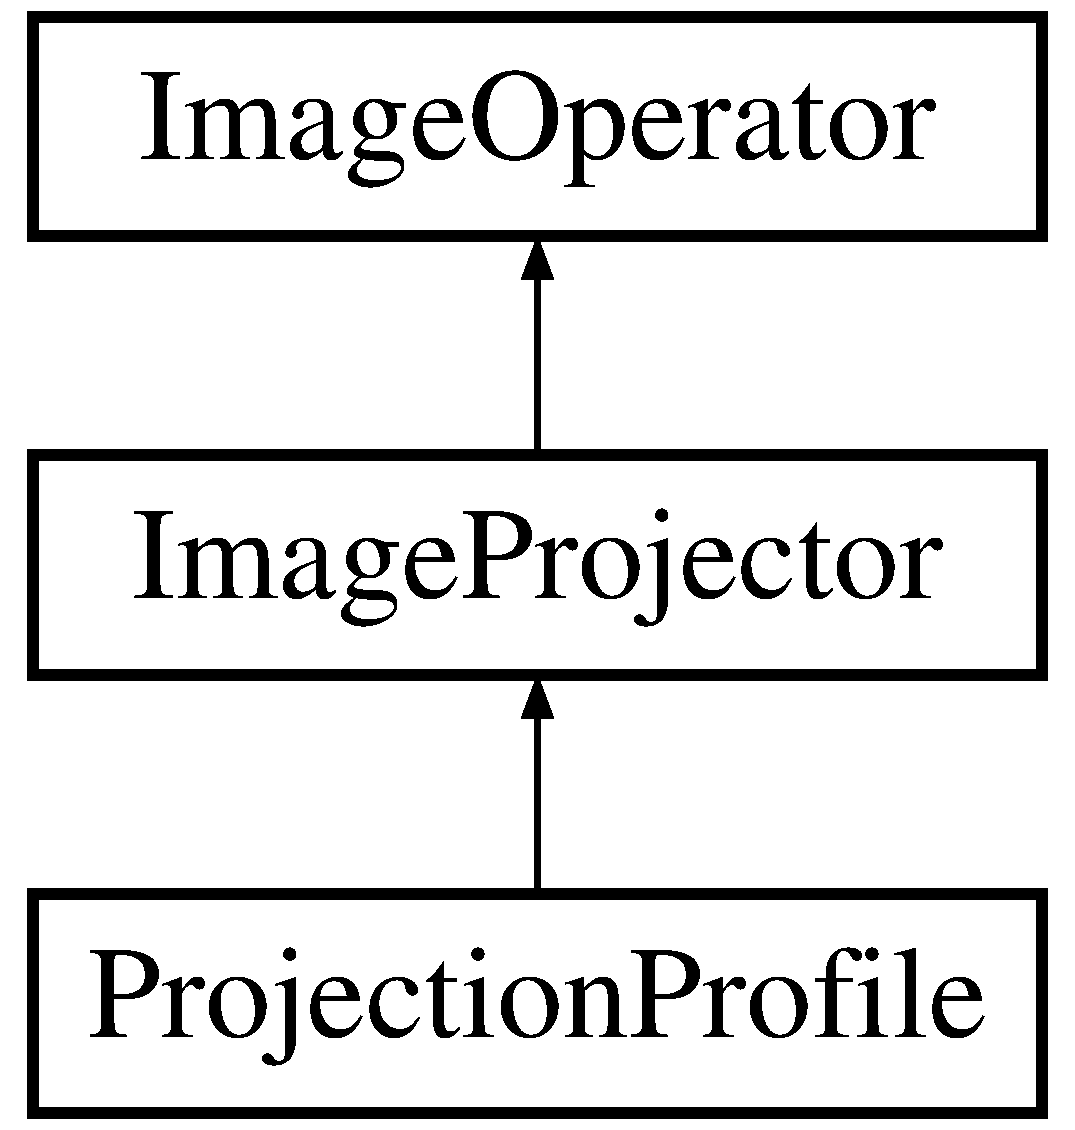
\includegraphics[height=3.000000cm]{class_projection_profile}
\end{center}
\end{figure}
\subsection*{Public Member Functions}
\begin{DoxyCompactItemize}
\item 
\hyperlink{class_projection_profile_a731890565b59cf377deb0c09638216c9}{Projection\+Profile} ()
\item 
\hyperlink{class_projection_profile_aefd5810dbfc34bddd1c7fedb539d6996}{Projection\+Profile} (int mode)
\item 
\hyperlink{class_projection_profile_ab901ba9a5572288f36e23f926ec85028}{$\sim$\+Projection\+Profile} (void)
\item 
void \hyperlink{class_projection_profile_a2f196aaeff36268a12033b0d35180c4d}{smooth\+Profile} (Mat profile)
\item 
void \hyperlink{class_projection_profile_a8bb3b2db0312483fc39ea60cb0067612}{draw\+Profile} (\hyperlink{class_d_image}{D\+Image} $\ast$img, \hyperlink{class_d_image}{D\+Image} $\ast$profile, int width)
\item 
vector$<$ \hyperlink{_projection_profile_8h_a9d6aea485bdd024cbf1618a864c0dc50}{Extremum} $>$ \hyperlink{class_projection_profile_ad3ee9dbf2b9a932fc5e2e591b1d9e693}{find\+Minimum\+Maximum} (\hyperlink{class_d_image}{D\+Image} $\ast$profile)
\item 
double \hyperlink{class_projection_profile_a558047469b18ba1fa1ae3ffd98e3c491}{get\+Weight} (\hyperlink{class_d_image}{D\+Image} $\ast$profile, int scheme)
\item 
\hyperlink{class_d_image}{D\+Image} $\ast$ \hyperlink{class_projection_profile_a876b05a649f497584fe5d5632ffab9c0}{project} ()
\begin{DoxyCompactList}\small\item\em Project a 2\+D image into 1\+D image (one column) \end{DoxyCompactList}\end{DoxyCompactItemize}
\subsection*{Static Public Attributes}
\begin{DoxyCompactItemize}
\item 
static const int \hyperlink{class_projection_profile_a06bb71f5459acefbdac42a661a4c494e}{W\+S\+\_\+\+S\+U\+M} = 0
\item 
static const int \hyperlink{class_projection_profile_a89ec8c60c23f878f08e27b0271e94153}{W\+S\+\_\+\+P\+E\+A\+K\+\_\+\+V\+A\+L\+Y\+\_\+\+D\+I\+F\+F} = 1
\end{DoxyCompactItemize}
\subsection*{Protected Member Functions}
\begin{DoxyCompactItemize}
\item 
double \hyperlink{class_projection_profile_a021b58fa03665d59cf6a21827a4c514c}{get\+Profile\+Sum} (\hyperlink{class_d_image}{D\+Image} $\ast$profile)
\item 
double \hyperlink{class_projection_profile_ae7f19afd842e2989b7642d4de8f7f334}{get\+Peak\+Valley\+Sum} (\hyperlink{class_d_image}{D\+Image} $\ast$profie)
\end{DoxyCompactItemize}
\subsection*{Additional Inherited Members}


\subsection{Constructor \& Destructor Documentation}
\hypertarget{class_projection_profile_a731890565b59cf377deb0c09638216c9}{\index{Projection\+Profile@{Projection\+Profile}!Projection\+Profile@{Projection\+Profile}}
\index{Projection\+Profile@{Projection\+Profile}!Projection\+Profile@{Projection\+Profile}}
\subsubsection[{Projection\+Profile}]{\setlength{\rightskip}{0pt plus 5cm}Projection\+Profile\+::\+Projection\+Profile (
\begin{DoxyParamCaption}
{}
\end{DoxyParamCaption}
)\hspace{0.3cm}{\ttfamily [inline]}}}\label{class_projection_profile_a731890565b59cf377deb0c09638216c9}
\hypertarget{class_projection_profile_aefd5810dbfc34bddd1c7fedb539d6996}{\index{Projection\+Profile@{Projection\+Profile}!Projection\+Profile@{Projection\+Profile}}
\index{Projection\+Profile@{Projection\+Profile}!Projection\+Profile@{Projection\+Profile}}
\subsubsection[{Projection\+Profile}]{\setlength{\rightskip}{0pt plus 5cm}Projection\+Profile\+::\+Projection\+Profile (
\begin{DoxyParamCaption}
\item[{int}]{mode}
\end{DoxyParamCaption}
)\hspace{0.3cm}{\ttfamily [inline]}}}\label{class_projection_profile_aefd5810dbfc34bddd1c7fedb539d6996}
\hypertarget{class_projection_profile_ab901ba9a5572288f36e23f926ec85028}{\index{Projection\+Profile@{Projection\+Profile}!````~Projection\+Profile@{$\sim$\+Projection\+Profile}}
\index{````~Projection\+Profile@{$\sim$\+Projection\+Profile}!Projection\+Profile@{Projection\+Profile}}
\subsubsection[{$\sim$\+Projection\+Profile}]{\setlength{\rightskip}{0pt plus 5cm}Projection\+Profile\+::$\sim$\+Projection\+Profile (
\begin{DoxyParamCaption}
\item[{void}]{}
\end{DoxyParamCaption}
)\hspace{0.3cm}{\ttfamily [inline]}}}\label{class_projection_profile_ab901ba9a5572288f36e23f926ec85028}


\subsection{Member Function Documentation}
\hypertarget{class_projection_profile_a8bb3b2db0312483fc39ea60cb0067612}{\index{Projection\+Profile@{Projection\+Profile}!draw\+Profile@{draw\+Profile}}
\index{draw\+Profile@{draw\+Profile}!Projection\+Profile@{Projection\+Profile}}
\subsubsection[{draw\+Profile}]{\setlength{\rightskip}{0pt plus 5cm}void Projection\+Profile\+::draw\+Profile (
\begin{DoxyParamCaption}
\item[{{\bf D\+Image} $\ast$}]{img, }
\item[{{\bf D\+Image} $\ast$}]{profile, }
\item[{int}]{width}
\end{DoxyParamCaption}
)}}\label{class_projection_profile_a8bb3b2db0312483fc39ea60cb0067612}
\hypertarget{class_projection_profile_ad3ee9dbf2b9a932fc5e2e591b1d9e693}{\index{Projection\+Profile@{Projection\+Profile}!find\+Minimum\+Maximum@{find\+Minimum\+Maximum}}
\index{find\+Minimum\+Maximum@{find\+Minimum\+Maximum}!Projection\+Profile@{Projection\+Profile}}
\subsubsection[{find\+Minimum\+Maximum}]{\setlength{\rightskip}{0pt plus 5cm}std\+::vector$<$ std\+::pair$<$ Point2i, bool $>$ $>$ Projection\+Profile\+::find\+Minimum\+Maximum (
\begin{DoxyParamCaption}
\item[{{\bf D\+Image} $\ast$}]{profile}
\end{DoxyParamCaption}
)}}\label{class_projection_profile_ad3ee9dbf2b9a932fc5e2e591b1d9e693}
\hypertarget{class_projection_profile_ae7f19afd842e2989b7642d4de8f7f334}{\index{Projection\+Profile@{Projection\+Profile}!get\+Peak\+Valley\+Sum@{get\+Peak\+Valley\+Sum}}
\index{get\+Peak\+Valley\+Sum@{get\+Peak\+Valley\+Sum}!Projection\+Profile@{Projection\+Profile}}
\subsubsection[{get\+Peak\+Valley\+Sum}]{\setlength{\rightskip}{0pt plus 5cm}double Projection\+Profile\+::get\+Peak\+Valley\+Sum (
\begin{DoxyParamCaption}
\item[{{\bf D\+Image} $\ast$}]{profie}
\end{DoxyParamCaption}
)\hspace{0.3cm}{\ttfamily [protected]}}}\label{class_projection_profile_ae7f19afd842e2989b7642d4de8f7f334}
\hypertarget{class_projection_profile_a021b58fa03665d59cf6a21827a4c514c}{\index{Projection\+Profile@{Projection\+Profile}!get\+Profile\+Sum@{get\+Profile\+Sum}}
\index{get\+Profile\+Sum@{get\+Profile\+Sum}!Projection\+Profile@{Projection\+Profile}}
\subsubsection[{get\+Profile\+Sum}]{\setlength{\rightskip}{0pt plus 5cm}double Projection\+Profile\+::get\+Profile\+Sum (
\begin{DoxyParamCaption}
\item[{{\bf D\+Image} $\ast$}]{profile}
\end{DoxyParamCaption}
)\hspace{0.3cm}{\ttfamily [protected]}}}\label{class_projection_profile_a021b58fa03665d59cf6a21827a4c514c}
\hypertarget{class_projection_profile_a558047469b18ba1fa1ae3ffd98e3c491}{\index{Projection\+Profile@{Projection\+Profile}!get\+Weight@{get\+Weight}}
\index{get\+Weight@{get\+Weight}!Projection\+Profile@{Projection\+Profile}}
\subsubsection[{get\+Weight}]{\setlength{\rightskip}{0pt plus 5cm}double Projection\+Profile\+::get\+Weight (
\begin{DoxyParamCaption}
\item[{{\bf D\+Image} $\ast$}]{profile, }
\item[{int}]{scheme}
\end{DoxyParamCaption}
)}}\label{class_projection_profile_a558047469b18ba1fa1ae3ffd98e3c491}
\hypertarget{class_projection_profile_a876b05a649f497584fe5d5632ffab9c0}{\index{Projection\+Profile@{Projection\+Profile}!project@{project}}
\index{project@{project}!Projection\+Profile@{Projection\+Profile}}
\subsubsection[{project}]{\setlength{\rightskip}{0pt plus 5cm}{\bf D\+Image} $\ast$ Projection\+Profile\+::project (
\begin{DoxyParamCaption}
{}
\end{DoxyParamCaption}
)\hspace{0.3cm}{\ttfamily [virtual]}}}\label{class_projection_profile_a876b05a649f497584fe5d5632ffab9c0}


Project a 2\+D image into 1\+D image (one column) 

El Sana. 


\begin{DoxyParams}{Parameters}
{\em img} & \mbox{[}in\mbox{]} The image. \\
\hline
\end{DoxyParams}


Implements \hyperlink{class_image_projector_a3dd19fda98e15001d7cbf5b8ca1b4b40}{Image\+Projector}.

\hypertarget{class_projection_profile_a2f196aaeff36268a12033b0d35180c4d}{\index{Projection\+Profile@{Projection\+Profile}!smooth\+Profile@{smooth\+Profile}}
\index{smooth\+Profile@{smooth\+Profile}!Projection\+Profile@{Projection\+Profile}}
\subsubsection[{smooth\+Profile}]{\setlength{\rightskip}{0pt plus 5cm}void Projection\+Profile\+::smooth\+Profile (
\begin{DoxyParamCaption}
\item[{Mat}]{profile}
\end{DoxyParamCaption}
)\hspace{0.3cm}{\ttfamily [inline]}}}\label{class_projection_profile_a2f196aaeff36268a12033b0d35180c4d}


\subsection{Member Data Documentation}
\hypertarget{class_projection_profile_a89ec8c60c23f878f08e27b0271e94153}{\index{Projection\+Profile@{Projection\+Profile}!W\+S\+\_\+\+P\+E\+A\+K\+\_\+\+V\+A\+L\+Y\+\_\+\+D\+I\+F\+F@{W\+S\+\_\+\+P\+E\+A\+K\+\_\+\+V\+A\+L\+Y\+\_\+\+D\+I\+F\+F}}
\index{W\+S\+\_\+\+P\+E\+A\+K\+\_\+\+V\+A\+L\+Y\+\_\+\+D\+I\+F\+F@{W\+S\+\_\+\+P\+E\+A\+K\+\_\+\+V\+A\+L\+Y\+\_\+\+D\+I\+F\+F}!Projection\+Profile@{Projection\+Profile}}
\subsubsection[{W\+S\+\_\+\+P\+E\+A\+K\+\_\+\+V\+A\+L\+Y\+\_\+\+D\+I\+F\+F}]{\setlength{\rightskip}{0pt plus 5cm}const int Projection\+Profile\+::\+W\+S\+\_\+\+P\+E\+A\+K\+\_\+\+V\+A\+L\+Y\+\_\+\+D\+I\+F\+F = 1\hspace{0.3cm}{\ttfamily [static]}}}\label{class_projection_profile_a89ec8c60c23f878f08e27b0271e94153}
\hypertarget{class_projection_profile_a06bb71f5459acefbdac42a661a4c494e}{\index{Projection\+Profile@{Projection\+Profile}!W\+S\+\_\+\+S\+U\+M@{W\+S\+\_\+\+S\+U\+M}}
\index{W\+S\+\_\+\+S\+U\+M@{W\+S\+\_\+\+S\+U\+M}!Projection\+Profile@{Projection\+Profile}}
\subsubsection[{W\+S\+\_\+\+S\+U\+M}]{\setlength{\rightskip}{0pt plus 5cm}const int Projection\+Profile\+::\+W\+S\+\_\+\+S\+U\+M = 0\hspace{0.3cm}{\ttfamily [static]}}}\label{class_projection_profile_a06bb71f5459acefbdac42a661a4c494e}


The documentation for this class was generated from the following files\+:\begin{DoxyCompactItemize}
\item 
Manuscript\+App/\hyperlink{_projection_profile_8h}{Projection\+Profile.\+h}\item 
Manuscript\+App/\hyperlink{_projection_profile_8cpp}{Projection\+Profile.\+cpp}\end{DoxyCompactItemize}

\hypertarget{class_rafi_text_line_extractor}{\section{Rafi\+Text\+Line\+Extractor Class Reference}
\label{class_rafi_text_line_extractor}\index{Rafi\+Text\+Line\+Extractor@{Rafi\+Text\+Line\+Extractor}}
}


{\ttfamily \#include $<$Rafi\+Text\+Line\+Extractor.\+h$>$}

Inheritance diagram for Rafi\+Text\+Line\+Extractor\+:\begin{figure}[H]
\begin{center}
\leavevmode
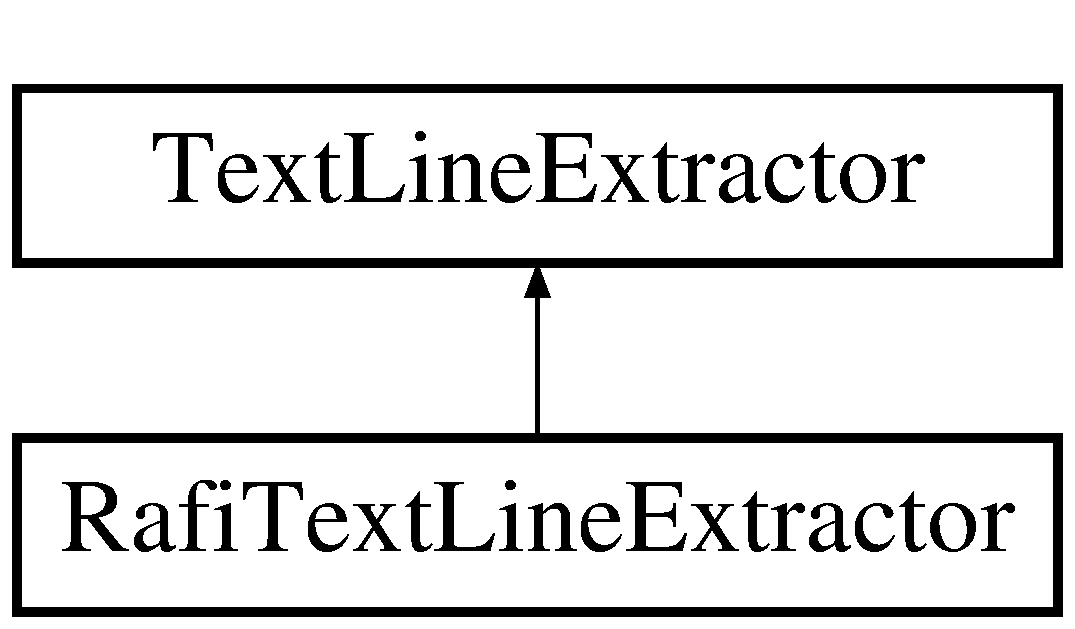
\includegraphics[height=2.000000cm]{class_rafi_text_line_extractor}
\end{center}
\end{figure}
\subsection*{Public Member Functions}
\begin{DoxyCompactItemize}
\item 
void \hyperlink{class_rafi_text_line_extractor_a96292e5e16014f1e48cf4754bf130d1f}{Traverse\+Tree} ()
\item 
\hyperlink{class_rafi_text_line_extractor_a7bbeb76ff90b68710376be91fddb95c9}{Rafi\+Text\+Line\+Extractor} ()
\item 
void \hyperlink{class_rafi_text_line_extractor_aec2e65306e243dfdf0675fb6987ff730}{extract} ()
\end{DoxyCompactItemize}
\subsection*{Protected Member Functions}
\begin{DoxyCompactItemize}
\item 
Mat \hyperlink{class_rafi_text_line_extractor_a4a5f293ba87e2c80d9e02b38050351ea}{filter\+Document} ()
\end{DoxyCompactItemize}
\subsection*{Additional Inherited Members}


\subsection{Constructor \& Destructor Documentation}
\hypertarget{class_rafi_text_line_extractor_a7bbeb76ff90b68710376be91fddb95c9}{\index{Rafi\+Text\+Line\+Extractor@{Rafi\+Text\+Line\+Extractor}!Rafi\+Text\+Line\+Extractor@{Rafi\+Text\+Line\+Extractor}}
\index{Rafi\+Text\+Line\+Extractor@{Rafi\+Text\+Line\+Extractor}!Rafi\+Text\+Line\+Extractor@{Rafi\+Text\+Line\+Extractor}}
\subsubsection[{Rafi\+Text\+Line\+Extractor}]{\setlength{\rightskip}{0pt plus 5cm}Rafi\+Text\+Line\+Extractor\+::\+Rafi\+Text\+Line\+Extractor (
\begin{DoxyParamCaption}
{}
\end{DoxyParamCaption}
)}}\label{class_rafi_text_line_extractor_a7bbeb76ff90b68710376be91fddb95c9}


\subsection{Member Function Documentation}
\hypertarget{class_rafi_text_line_extractor_aec2e65306e243dfdf0675fb6987ff730}{\index{Rafi\+Text\+Line\+Extractor@{Rafi\+Text\+Line\+Extractor}!extract@{extract}}
\index{extract@{extract}!Rafi\+Text\+Line\+Extractor@{Rafi\+Text\+Line\+Extractor}}
\subsubsection[{extract}]{\setlength{\rightskip}{0pt plus 5cm}void Rafi\+Text\+Line\+Extractor\+::extract (
\begin{DoxyParamCaption}
{}
\end{DoxyParamCaption}
)\hspace{0.3cm}{\ttfamily [virtual]}}}\label{class_rafi_text_line_extractor_aec2e65306e243dfdf0675fb6987ff730}


Implements \hyperlink{class_text_line_extractor_ae3e60f7dfccd378b6144510b5b85104f}{Text\+Line\+Extractor}.

\hypertarget{class_rafi_text_line_extractor_a4a5f293ba87e2c80d9e02b38050351ea}{\index{Rafi\+Text\+Line\+Extractor@{Rafi\+Text\+Line\+Extractor}!filter\+Document@{filter\+Document}}
\index{filter\+Document@{filter\+Document}!Rafi\+Text\+Line\+Extractor@{Rafi\+Text\+Line\+Extractor}}
\subsubsection[{filter\+Document}]{\setlength{\rightskip}{0pt plus 5cm}Mat Rafi\+Text\+Line\+Extractor\+::filter\+Document (
\begin{DoxyParamCaption}
{}
\end{DoxyParamCaption}
)\hspace{0.3cm}{\ttfamily [protected]}}}\label{class_rafi_text_line_extractor_a4a5f293ba87e2c80d9e02b38050351ea}
\hypertarget{class_rafi_text_line_extractor_a96292e5e16014f1e48cf4754bf130d1f}{\index{Rafi\+Text\+Line\+Extractor@{Rafi\+Text\+Line\+Extractor}!Traverse\+Tree@{Traverse\+Tree}}
\index{Traverse\+Tree@{Traverse\+Tree}!Rafi\+Text\+Line\+Extractor@{Rafi\+Text\+Line\+Extractor}}
\subsubsection[{Traverse\+Tree}]{\setlength{\rightskip}{0pt plus 5cm}void Rafi\+Text\+Line\+Extractor\+::\+Traverse\+Tree (
\begin{DoxyParamCaption}
{}
\end{DoxyParamCaption}
)}}\label{class_rafi_text_line_extractor_a96292e5e16014f1e48cf4754bf130d1f}


The documentation for this class was generated from the following files\+:\begin{DoxyCompactItemize}
\item 
Manuscript\+App/\hyperlink{_rafi_text_line_extractor_8h}{Rafi\+Text\+Line\+Extractor.\+h}\item 
Manuscript\+App/\hyperlink{_rafi_text_line_extractor_8cpp}{Rafi\+Text\+Line\+Extractor.\+cpp}\end{DoxyCompactItemize}

\hypertarget{class_scalar_feature}{\section{Scalar\+Feature$<$ T $>$ Class Template Reference}
\label{class_scalar_feature}\index{Scalar\+Feature$<$ T $>$@{Scalar\+Feature$<$ T $>$}}
}


{\ttfamily \#include $<$Scalar\+Feature.\+h$>$}

Inheritance diagram for Scalar\+Feature$<$ T $>$\+:\begin{figure}[H]
\begin{center}
\leavevmode
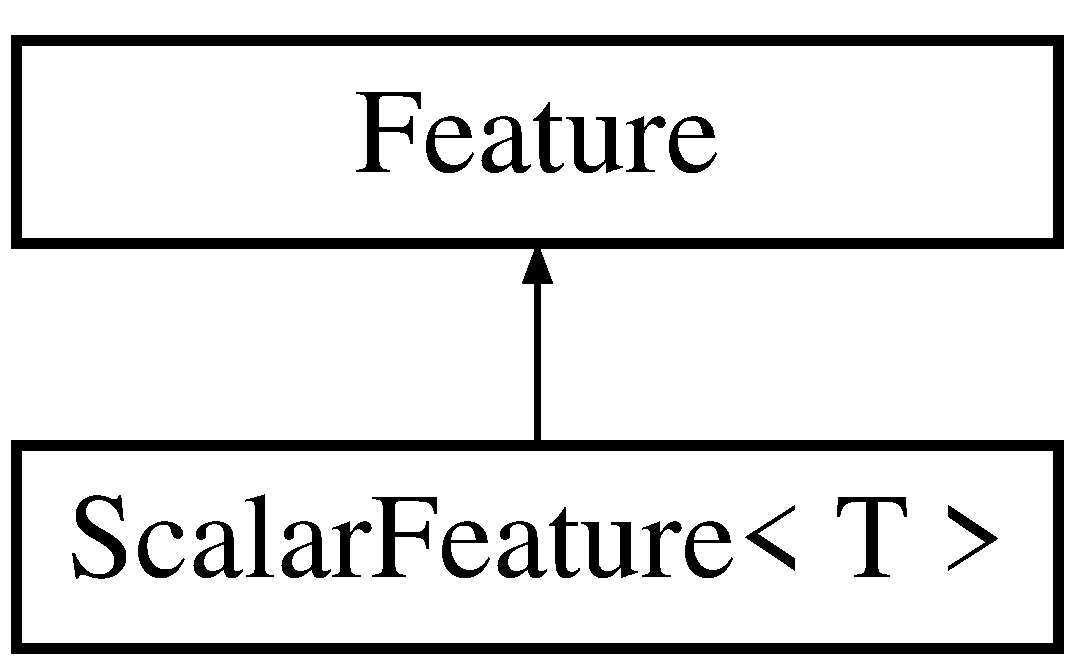
\includegraphics[height=2.000000cm]{class_scalar_feature}
\end{center}
\end{figure}
\subsection*{Public Member Functions}
\begin{DoxyCompactItemize}
\item 
\hyperlink{class_scalar_feature_aa1daecc3065ef533e347b81290b710e3}{Scalar\+Feature} ()
\item 
\hyperlink{class_scalar_feature_ace56cbb8d2624c2f8eb9a0d2f9fc7873}{Scalar\+Feature} (int a)
\item 
void \hyperlink{class_scalar_feature_ac8f206ffcbb1c71d4ac5877193d2d26b}{val} (T a)
\item 
T \hyperlink{class_scalar_feature_a504181db619359cb45ab8e2de509fb6e}{val} ()
\item 
double \hyperlink{class_scalar_feature_a5b95859a0d7409d7d9306a0c262e8e17}{distance} (\hyperlink{class_feature}{Feature} $\ast$a)
\end{DoxyCompactItemize}


\subsection{Constructor \& Destructor Documentation}
\hypertarget{class_scalar_feature_aa1daecc3065ef533e347b81290b710e3}{\index{Scalar\+Feature@{Scalar\+Feature}!Scalar\+Feature@{Scalar\+Feature}}
\index{Scalar\+Feature@{Scalar\+Feature}!Scalar\+Feature@{Scalar\+Feature}}
\subsubsection[{Scalar\+Feature}]{\setlength{\rightskip}{0pt plus 5cm}template$<$class T $>$ {\bf Scalar\+Feature}$<$ T $>$\+::{\bf Scalar\+Feature} (
\begin{DoxyParamCaption}
{}
\end{DoxyParamCaption}
)\hspace{0.3cm}{\ttfamily [inline]}}}\label{class_scalar_feature_aa1daecc3065ef533e347b81290b710e3}
\hypertarget{class_scalar_feature_ace56cbb8d2624c2f8eb9a0d2f9fc7873}{\index{Scalar\+Feature@{Scalar\+Feature}!Scalar\+Feature@{Scalar\+Feature}}
\index{Scalar\+Feature@{Scalar\+Feature}!Scalar\+Feature@{Scalar\+Feature}}
\subsubsection[{Scalar\+Feature}]{\setlength{\rightskip}{0pt plus 5cm}template$<$class T $>$ {\bf Scalar\+Feature}$<$ T $>$\+::{\bf Scalar\+Feature} (
\begin{DoxyParamCaption}
\item[{int}]{a}
\end{DoxyParamCaption}
)\hspace{0.3cm}{\ttfamily [inline]}}}\label{class_scalar_feature_ace56cbb8d2624c2f8eb9a0d2f9fc7873}


\subsection{Member Function Documentation}
\hypertarget{class_scalar_feature_a5b95859a0d7409d7d9306a0c262e8e17}{\index{Scalar\+Feature@{Scalar\+Feature}!distance@{distance}}
\index{distance@{distance}!Scalar\+Feature@{Scalar\+Feature}}
\subsubsection[{distance}]{\setlength{\rightskip}{0pt plus 5cm}template$<$class T $>$ double {\bf Scalar\+Feature}$<$ T $>$\+::distance (
\begin{DoxyParamCaption}
\item[{{\bf Feature} $\ast$}]{a}
\end{DoxyParamCaption}
)\hspace{0.3cm}{\ttfamily [inline]}, {\ttfamily [virtual]}}}\label{class_scalar_feature_a5b95859a0d7409d7d9306a0c262e8e17}


Implements \hyperlink{class_feature_a7dbbdc860cdc97bcd31584ae10dab3b1}{Feature}.

\hypertarget{class_scalar_feature_ac8f206ffcbb1c71d4ac5877193d2d26b}{\index{Scalar\+Feature@{Scalar\+Feature}!val@{val}}
\index{val@{val}!Scalar\+Feature@{Scalar\+Feature}}
\subsubsection[{val}]{\setlength{\rightskip}{0pt plus 5cm}template$<$class T $>$ void {\bf Scalar\+Feature}$<$ T $>$\+::val (
\begin{DoxyParamCaption}
\item[{T}]{a}
\end{DoxyParamCaption}
)\hspace{0.3cm}{\ttfamily [inline]}}}\label{class_scalar_feature_ac8f206ffcbb1c71d4ac5877193d2d26b}
\hypertarget{class_scalar_feature_a504181db619359cb45ab8e2de509fb6e}{\index{Scalar\+Feature@{Scalar\+Feature}!val@{val}}
\index{val@{val}!Scalar\+Feature@{Scalar\+Feature}}
\subsubsection[{val}]{\setlength{\rightskip}{0pt plus 5cm}template$<$class T $>$ T {\bf Scalar\+Feature}$<$ T $>$\+::val (
\begin{DoxyParamCaption}
{}
\end{DoxyParamCaption}
)\hspace{0.3cm}{\ttfamily [inline]}}}\label{class_scalar_feature_a504181db619359cb45ab8e2de509fb6e}


The documentation for this class was generated from the following file\+:\begin{DoxyCompactItemize}
\item 
Manuscript\+App/\hyperlink{_scalar_feature_8h}{Scalar\+Feature.\+h}\end{DoxyCompactItemize}

\hypertarget{class_text_line_extractor}{\section{Text\+Line\+Extractor Class Reference}
\label{class_text_line_extractor}\index{Text\+Line\+Extractor@{Text\+Line\+Extractor}}
}


Text line extractor is a base class for text line extraction algorithms. Each should implement the virtual funxtion extract  




{\ttfamily \#include $<$Text\+Line\+Extractor.\+h$>$}

Inheritance diagram for Text\+Line\+Extractor\+:\begin{figure}[H]
\begin{center}
\leavevmode
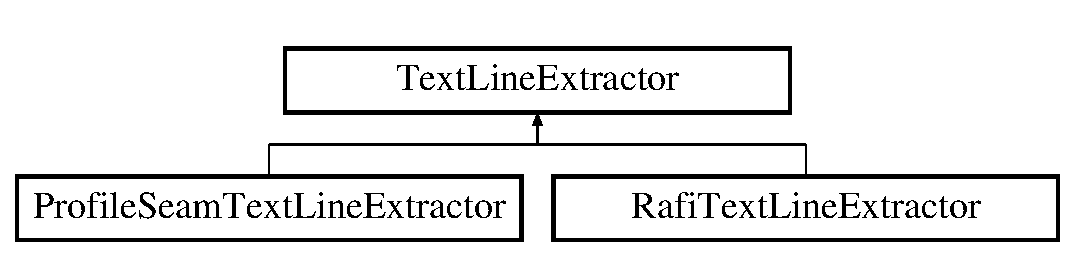
\includegraphics[height=2.000000cm]{class_text_line_extractor}
\end{center}
\end{figure}
\subsection*{Public Member Functions}
\begin{DoxyCompactItemize}
\item 
\hyperlink{class_text_line_extractor_a5f0c3627efd8b25b82e747a191b21d54}{Text\+Line\+Extractor} (void)
\item 
\hyperlink{class_text_line_extractor_a220ed917eeb0ded278f9a08539149623}{$\sim$\+Text\+Line\+Extractor} (void)
\item 
void \hyperlink{class_text_line_extractor_a67f7e8bdb62bff99de9816b55de4c6d0}{set\+Image} (Mat img)
\item 
virtual void \hyperlink{class_text_line_extractor_ae3e60f7dfccd378b6144510b5b85104f}{extract} ()=0
\end{DoxyCompactItemize}
\subsection*{Protected Attributes}
\begin{DoxyCompactItemize}
\item 
Mat \hyperlink{class_text_line_extractor_acc518adbefc6a211ce84f5124da31709}{\+\_\+image}
\end{DoxyCompactItemize}


\subsection{Detailed Description}
Text line extractor is a base class for text line extraction algorithms. Each should implement the virtual funxtion extract 

El Sana, 2/15/2012. 

\subsection{Constructor \& Destructor Documentation}
\hypertarget{class_text_line_extractor_a5f0c3627efd8b25b82e747a191b21d54}{\index{Text\+Line\+Extractor@{Text\+Line\+Extractor}!Text\+Line\+Extractor@{Text\+Line\+Extractor}}
\index{Text\+Line\+Extractor@{Text\+Line\+Extractor}!Text\+Line\+Extractor@{Text\+Line\+Extractor}}
\subsubsection[{Text\+Line\+Extractor}]{\setlength{\rightskip}{0pt plus 5cm}Text\+Line\+Extractor\+::\+Text\+Line\+Extractor (
\begin{DoxyParamCaption}
\item[{void}]{}
\end{DoxyParamCaption}
)\hspace{0.3cm}{\ttfamily [inline]}}}\label{class_text_line_extractor_a5f0c3627efd8b25b82e747a191b21d54}
\hypertarget{class_text_line_extractor_a220ed917eeb0ded278f9a08539149623}{\index{Text\+Line\+Extractor@{Text\+Line\+Extractor}!````~Text\+Line\+Extractor@{$\sim$\+Text\+Line\+Extractor}}
\index{````~Text\+Line\+Extractor@{$\sim$\+Text\+Line\+Extractor}!Text\+Line\+Extractor@{Text\+Line\+Extractor}}
\subsubsection[{$\sim$\+Text\+Line\+Extractor}]{\setlength{\rightskip}{0pt plus 5cm}Text\+Line\+Extractor\+::$\sim$\+Text\+Line\+Extractor (
\begin{DoxyParamCaption}
\item[{void}]{}
\end{DoxyParamCaption}
)\hspace{0.3cm}{\ttfamily [inline]}}}\label{class_text_line_extractor_a220ed917eeb0ded278f9a08539149623}


\subsection{Member Function Documentation}
\hypertarget{class_text_line_extractor_ae3e60f7dfccd378b6144510b5b85104f}{\index{Text\+Line\+Extractor@{Text\+Line\+Extractor}!extract@{extract}}
\index{extract@{extract}!Text\+Line\+Extractor@{Text\+Line\+Extractor}}
\subsubsection[{extract}]{\setlength{\rightskip}{0pt plus 5cm}virtual void Text\+Line\+Extractor\+::extract (
\begin{DoxyParamCaption}
{}
\end{DoxyParamCaption}
)\hspace{0.3cm}{\ttfamily [pure virtual]}}}\label{class_text_line_extractor_ae3e60f7dfccd378b6144510b5b85104f}


Implemented in \hyperlink{class_profile_seam_text_line_extractor_a67017476e961c0531524d3f52cf70e23}{Profile\+Seam\+Text\+Line\+Extractor}, and \hyperlink{class_rafi_text_line_extractor_aec2e65306e243dfdf0675fb6987ff730}{Rafi\+Text\+Line\+Extractor}.

\hypertarget{class_text_line_extractor_a67f7e8bdb62bff99de9816b55de4c6d0}{\index{Text\+Line\+Extractor@{Text\+Line\+Extractor}!set\+Image@{set\+Image}}
\index{set\+Image@{set\+Image}!Text\+Line\+Extractor@{Text\+Line\+Extractor}}
\subsubsection[{set\+Image}]{\setlength{\rightskip}{0pt plus 5cm}void Text\+Line\+Extractor\+::set\+Image (
\begin{DoxyParamCaption}
\item[{Mat}]{img}
\end{DoxyParamCaption}
)\hspace{0.3cm}{\ttfamily [inline]}}}\label{class_text_line_extractor_a67f7e8bdb62bff99de9816b55de4c6d0}


\subsection{Member Data Documentation}
\hypertarget{class_text_line_extractor_acc518adbefc6a211ce84f5124da31709}{\index{Text\+Line\+Extractor@{Text\+Line\+Extractor}!\+\_\+image@{\+\_\+image}}
\index{\+\_\+image@{\+\_\+image}!Text\+Line\+Extractor@{Text\+Line\+Extractor}}
\subsubsection[{\+\_\+image}]{\setlength{\rightskip}{0pt plus 5cm}Mat Text\+Line\+Extractor\+::\+\_\+image\hspace{0.3cm}{\ttfamily [protected]}}}\label{class_text_line_extractor_acc518adbefc6a211ce84f5124da31709}


The documentation for this class was generated from the following file\+:\begin{DoxyCompactItemize}
\item 
Manuscript\+App/\hyperlink{_text_line_extractor_8h}{Text\+Line\+Extractor.\+h}\end{DoxyCompactItemize}

\hypertarget{class_threshold_binarizer}{\section{Threshold\+Binarizer Class Reference}
\label{class_threshold_binarizer}\index{Threshold\+Binarizer@{Threshold\+Binarizer}}
}


{\ttfamily \#include $<$Threshold\+Binarizer.\+h$>$}

Inheritance diagram for Threshold\+Binarizer\+:\begin{figure}[H]
\begin{center}
\leavevmode
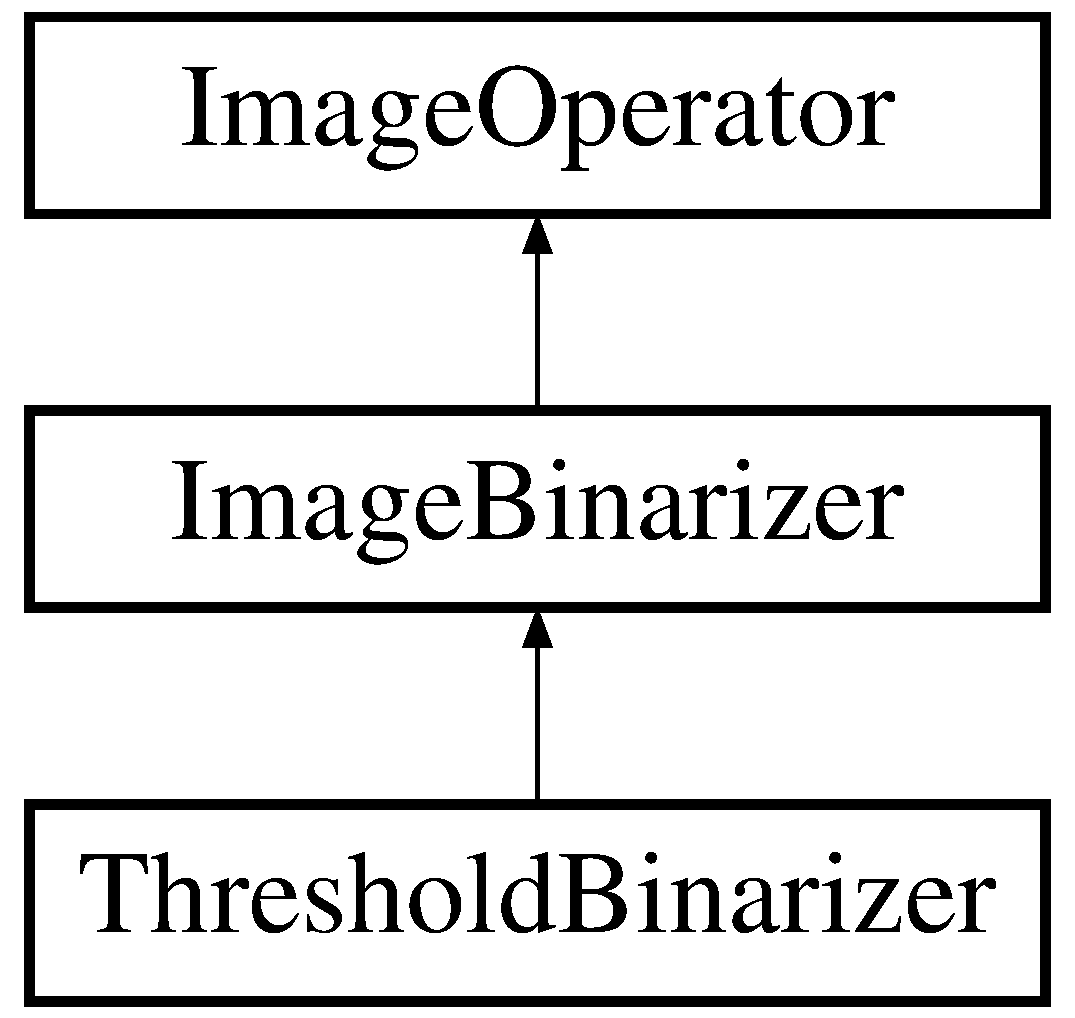
\includegraphics[height=3.000000cm]{class_threshold_binarizer}
\end{center}
\end{figure}
\subsection*{Public Member Functions}
\begin{DoxyCompactItemize}
\item 
\hyperlink{class_threshold_binarizer_a951304a610f67e3ba71823f4a376111a}{Threshold\+Binarizer} (int threshold)
\item 
\hyperlink{class_threshold_binarizer_adcca8ae82313ed16e17f06d27abdf9b5}{Threshold\+Binarizer} (int threshold, bool reverse)
\item 
void \hyperlink{class_threshold_binarizer_a6e58690b08f2db45e4235b44629ae307}{set\+Threshold} (int threshold)
\item 
void \hyperlink{class_threshold_binarizer_a6dbfb62c3bc1a692dfd220743ef006cc}{set\+Reverse} (bool reverse)
\item 
\hyperlink{class_d_image}{D\+Image} $\ast$ \hyperlink{class_threshold_binarizer_a2880414f620b4a6f44032e478217ee1e}{binarize} ()
\begin{DoxyCompactList}\small\item\em binarize an image based on a thershold \end{DoxyCompactList}\end{DoxyCompactItemize}
\subsection*{Additional Inherited Members}


\subsection{Constructor \& Destructor Documentation}
\hypertarget{class_threshold_binarizer_a951304a610f67e3ba71823f4a376111a}{\index{Threshold\+Binarizer@{Threshold\+Binarizer}!Threshold\+Binarizer@{Threshold\+Binarizer}}
\index{Threshold\+Binarizer@{Threshold\+Binarizer}!Threshold\+Binarizer@{Threshold\+Binarizer}}
\subsubsection[{Threshold\+Binarizer}]{\setlength{\rightskip}{0pt plus 5cm}Threshold\+Binarizer\+::\+Threshold\+Binarizer (
\begin{DoxyParamCaption}
\item[{int}]{threshold}
\end{DoxyParamCaption}
)\hspace{0.3cm}{\ttfamily [inline]}}}\label{class_threshold_binarizer_a951304a610f67e3ba71823f4a376111a}
\hypertarget{class_threshold_binarizer_adcca8ae82313ed16e17f06d27abdf9b5}{\index{Threshold\+Binarizer@{Threshold\+Binarizer}!Threshold\+Binarizer@{Threshold\+Binarizer}}
\index{Threshold\+Binarizer@{Threshold\+Binarizer}!Threshold\+Binarizer@{Threshold\+Binarizer}}
\subsubsection[{Threshold\+Binarizer}]{\setlength{\rightskip}{0pt plus 5cm}Threshold\+Binarizer\+::\+Threshold\+Binarizer (
\begin{DoxyParamCaption}
\item[{int}]{threshold, }
\item[{bool}]{reverse}
\end{DoxyParamCaption}
)\hspace{0.3cm}{\ttfamily [inline]}}}\label{class_threshold_binarizer_adcca8ae82313ed16e17f06d27abdf9b5}


\subsection{Member Function Documentation}
\hypertarget{class_threshold_binarizer_a2880414f620b4a6f44032e478217ee1e}{\index{Threshold\+Binarizer@{Threshold\+Binarizer}!binarize@{binarize}}
\index{binarize@{binarize}!Threshold\+Binarizer@{Threshold\+Binarizer}}
\subsubsection[{binarize}]{\setlength{\rightskip}{0pt plus 5cm}{\bf D\+Image} $\ast$ Threshold\+Binarizer\+::binarize (
\begin{DoxyParamCaption}
{}
\end{DoxyParamCaption}
)\hspace{0.3cm}{\ttfamily [virtual]}}}\label{class_threshold_binarizer_a2880414f620b4a6f44032e478217ee1e}


binarize an image based on a thershold 

El Sana, 2/15/2012. 

\begin{DoxyReturn}{Returns}
null if it fails, else. 
\end{DoxyReturn}


Implements \hyperlink{class_image_binarizer_accf059357ade25887a94c91f76262254}{Image\+Binarizer}.

\hypertarget{class_threshold_binarizer_a6dbfb62c3bc1a692dfd220743ef006cc}{\index{Threshold\+Binarizer@{Threshold\+Binarizer}!set\+Reverse@{set\+Reverse}}
\index{set\+Reverse@{set\+Reverse}!Threshold\+Binarizer@{Threshold\+Binarizer}}
\subsubsection[{set\+Reverse}]{\setlength{\rightskip}{0pt plus 5cm}void Threshold\+Binarizer\+::set\+Reverse (
\begin{DoxyParamCaption}
\item[{bool}]{reverse}
\end{DoxyParamCaption}
)\hspace{0.3cm}{\ttfamily [inline]}}}\label{class_threshold_binarizer_a6dbfb62c3bc1a692dfd220743ef006cc}
\hypertarget{class_threshold_binarizer_a6e58690b08f2db45e4235b44629ae307}{\index{Threshold\+Binarizer@{Threshold\+Binarizer}!set\+Threshold@{set\+Threshold}}
\index{set\+Threshold@{set\+Threshold}!Threshold\+Binarizer@{Threshold\+Binarizer}}
\subsubsection[{set\+Threshold}]{\setlength{\rightskip}{0pt plus 5cm}void Threshold\+Binarizer\+::set\+Threshold (
\begin{DoxyParamCaption}
\item[{int}]{threshold}
\end{DoxyParamCaption}
)\hspace{0.3cm}{\ttfamily [inline]}}}\label{class_threshold_binarizer_a6e58690b08f2db45e4235b44629ae307}


The documentation for this class was generated from the following files\+:\begin{DoxyCompactItemize}
\item 
Manuscript\+App/\hyperlink{_threshold_binarizer_8h}{Threshold\+Binarizer.\+h}\item 
Manuscript\+App/\hyperlink{_threshold_binarizer_8cpp}{Threshold\+Binarizer.\+cpp}\end{DoxyCompactItemize}

\chapter{File Documentation}
\hypertarget{anigauss_8h}{\section{Manuscript\+App/anigauss.h File Reference}
\label{anigauss_8h}\index{Manuscript\+App/anigauss.\+h@{Manuscript\+App/anigauss.\+h}}
}
{\ttfamily \#include $<$math.\+h$>$}\\*
{\ttfamily \#include $<$stdlib.\+h$>$}\\*
\subsection*{Macros}
\begin{DoxyCompactItemize}
\item 
\#define \hyperlink{anigauss_8h_a598a3330b3c21701223ee0ca14316eca}{P\+I}~3.\+14159265358979323846
\item 
\#define \hyperlink{anigauss_8h_af6cd02292ac5596aabfe6f66d3758aac}{S\+R\+C\+T\+Y\+P\+E}~double
\item 
\#define \hyperlink{anigauss_8h_a1eefe9e8a78002dee3e956f6a42a2015}{D\+S\+T\+T\+Y\+P\+E}~double
\end{DoxyCompactItemize}
\subsection*{Functions}
\begin{DoxyCompactItemize}
\item 
void \hyperlink{anigauss_8h_add0518151a7f774aae955a21358f1496}{Yv\+Vfilter\+Coef} (double sigma, double $\ast$filter)
\item 
void \hyperlink{anigauss_8h_a922a1e9ec611998813439d7ea7c28d3f}{Triggs\+M} (double $\ast$filter, double $\ast$M)
\item 
void \hyperlink{anigauss_8h_ae97e45541e212872609d2ad24f0672b8}{anigauss} (\hyperlink{anigauss_8h_af6cd02292ac5596aabfe6f66d3758aac}{S\+R\+C\+T\+Y\+P\+E} $\ast$input, \hyperlink{anigauss_8h_a1eefe9e8a78002dee3e956f6a42a2015}{D\+S\+T\+T\+Y\+P\+E} $\ast$output, int sizex, int sizey, double sigmav, double sigmau, double phi, int orderv, int orderu)
\end{DoxyCompactItemize}


\subsection{Macro Definition Documentation}
\hypertarget{anigauss_8h_a1eefe9e8a78002dee3e956f6a42a2015}{\index{anigauss.\+h@{anigauss.\+h}!D\+S\+T\+T\+Y\+P\+E@{D\+S\+T\+T\+Y\+P\+E}}
\index{D\+S\+T\+T\+Y\+P\+E@{D\+S\+T\+T\+Y\+P\+E}!anigauss.\+h@{anigauss.\+h}}
\subsubsection[{D\+S\+T\+T\+Y\+P\+E}]{\setlength{\rightskip}{0pt plus 5cm}\#define D\+S\+T\+T\+Y\+P\+E~double}}\label{anigauss_8h_a1eefe9e8a78002dee3e956f6a42a2015}
\hypertarget{anigauss_8h_a598a3330b3c21701223ee0ca14316eca}{\index{anigauss.\+h@{anigauss.\+h}!P\+I@{P\+I}}
\index{P\+I@{P\+I}!anigauss.\+h@{anigauss.\+h}}
\subsubsection[{P\+I}]{\setlength{\rightskip}{0pt plus 5cm}\#define P\+I~3.\+14159265358979323846}}\label{anigauss_8h_a598a3330b3c21701223ee0ca14316eca}
\hypertarget{anigauss_8h_af6cd02292ac5596aabfe6f66d3758aac}{\index{anigauss.\+h@{anigauss.\+h}!S\+R\+C\+T\+Y\+P\+E@{S\+R\+C\+T\+Y\+P\+E}}
\index{S\+R\+C\+T\+Y\+P\+E@{S\+R\+C\+T\+Y\+P\+E}!anigauss.\+h@{anigauss.\+h}}
\subsubsection[{S\+R\+C\+T\+Y\+P\+E}]{\setlength{\rightskip}{0pt plus 5cm}\#define S\+R\+C\+T\+Y\+P\+E~double}}\label{anigauss_8h_af6cd02292ac5596aabfe6f66d3758aac}


\subsection{Function Documentation}
\hypertarget{anigauss_8h_ae97e45541e212872609d2ad24f0672b8}{\index{anigauss.\+h@{anigauss.\+h}!anigauss@{anigauss}}
\index{anigauss@{anigauss}!anigauss.\+h@{anigauss.\+h}}
\subsubsection[{anigauss}]{\setlength{\rightskip}{0pt plus 5cm}void anigauss (
\begin{DoxyParamCaption}
\item[{{\bf S\+R\+C\+T\+Y\+P\+E} $\ast$}]{input, }
\item[{{\bf D\+S\+T\+T\+Y\+P\+E} $\ast$}]{output, }
\item[{int}]{sizex, }
\item[{int}]{sizey, }
\item[{double}]{sigmav, }
\item[{double}]{sigmau, }
\item[{double}]{phi, }
\item[{int}]{orderv, }
\item[{int}]{orderu}
\end{DoxyParamCaption}
)}}\label{anigauss_8h_ae97e45541e212872609d2ad24f0672b8}
\hypertarget{anigauss_8h_a922a1e9ec611998813439d7ea7c28d3f}{\index{anigauss.\+h@{anigauss.\+h}!Triggs\+M@{Triggs\+M}}
\index{Triggs\+M@{Triggs\+M}!anigauss.\+h@{anigauss.\+h}}
\subsubsection[{Triggs\+M}]{\setlength{\rightskip}{0pt plus 5cm}void Triggs\+M (
\begin{DoxyParamCaption}
\item[{double $\ast$}]{filter, }
\item[{double $\ast$}]{M}
\end{DoxyParamCaption}
)}}\label{anigauss_8h_a922a1e9ec611998813439d7ea7c28d3f}
\hypertarget{anigauss_8h_add0518151a7f774aae955a21358f1496}{\index{anigauss.\+h@{anigauss.\+h}!Yv\+Vfilter\+Coef@{Yv\+Vfilter\+Coef}}
\index{Yv\+Vfilter\+Coef@{Yv\+Vfilter\+Coef}!anigauss.\+h@{anigauss.\+h}}
\subsubsection[{Yv\+Vfilter\+Coef}]{\setlength{\rightskip}{0pt plus 5cm}void Yv\+Vfilter\+Coef (
\begin{DoxyParamCaption}
\item[{double}]{sigma, }
\item[{double $\ast$}]{filter}
\end{DoxyParamCaption}
)}}\label{anigauss_8h_add0518151a7f774aae955a21358f1496}

\hypertarget{_anisotropic_filter_8cpp}{\section{Manuscript\+App/\+Anisotropic\+Filter.cpp File Reference}
\label{_anisotropic_filter_8cpp}\index{Manuscript\+App/\+Anisotropic\+Filter.\+cpp@{Manuscript\+App/\+Anisotropic\+Filter.\+cpp}}
}
{\ttfamily \#include \char`\"{}stdafx.\+h\char`\"{}}\\*
{\ttfamily \#include \char`\"{}Anisotropic\+Filter.\+h\char`\"{}}\\*
{\ttfamily \#include \char`\"{}anigauss.\+h\char`\"{}}\\*
{\ttfamily \#include \char`\"{}Binary\+Component\+Extractor.\+h\char`\"{}}\\*
{\ttfamily \#include $<$math.\+h$>$}\\*

\hypertarget{_anisotropic_filter_8h}{\section{Manuscript\+App/\+Anisotropic\+Filter.h File Reference}
\label{_anisotropic_filter_8h}\index{Manuscript\+App/\+Anisotropic\+Filter.\+h@{Manuscript\+App/\+Anisotropic\+Filter.\+h}}
}
{\ttfamily \#include \char`\"{}D\+Image.\+h\char`\"{}}\\*
{\ttfamily \#include \char`\"{}Image\+Filter.\+h\char`\"{}}\\*
\subsection*{Classes}
\begin{DoxyCompactItemize}
\item 
class \hyperlink{class_anisotropic_filter}{Anisotropic\+Filter}
\end{DoxyCompactItemize}
\subsection*{Macros}
\begin{DoxyCompactItemize}
\item 
\#define \hyperlink{_anisotropic_filter_8h_add7587fa768b74eff9a321002fac911b}{\+\_\+\+A\+N\+I\+S\+O\+T\+R\+O\+P\+I\+C\+\_\+\+F\+I\+L\+T\+E\+R\+\_\+\+H\+\_\+}
\end{DoxyCompactItemize}


\subsection{Macro Definition Documentation}
\hypertarget{_anisotropic_filter_8h_add7587fa768b74eff9a321002fac911b}{\index{Anisotropic\+Filter.\+h@{Anisotropic\+Filter.\+h}!\+\_\+\+A\+N\+I\+S\+O\+T\+R\+O\+P\+I\+C\+\_\+\+F\+I\+L\+T\+E\+R\+\_\+\+H\+\_\+@{\+\_\+\+A\+N\+I\+S\+O\+T\+R\+O\+P\+I\+C\+\_\+\+F\+I\+L\+T\+E\+R\+\_\+\+H\+\_\+}}
\index{\+\_\+\+A\+N\+I\+S\+O\+T\+R\+O\+P\+I\+C\+\_\+\+F\+I\+L\+T\+E\+R\+\_\+\+H\+\_\+@{\+\_\+\+A\+N\+I\+S\+O\+T\+R\+O\+P\+I\+C\+\_\+\+F\+I\+L\+T\+E\+R\+\_\+\+H\+\_\+}!Anisotropic\+Filter.\+h@{Anisotropic\+Filter.\+h}}
\subsubsection[{\+\_\+\+A\+N\+I\+S\+O\+T\+R\+O\+P\+I\+C\+\_\+\+F\+I\+L\+T\+E\+R\+\_\+\+H\+\_\+}]{\setlength{\rightskip}{0pt plus 5cm}\#define \+\_\+\+A\+N\+I\+S\+O\+T\+R\+O\+P\+I\+C\+\_\+\+F\+I\+L\+T\+E\+R\+\_\+\+H\+\_\+}}\label{_anisotropic_filter_8h_add7587fa768b74eff9a321002fac911b}

\hypertarget{_binary_component_extractor_8cpp}{\section{Manuscript\+App/\+Binary\+Component\+Extractor.cpp File Reference}
\label{_binary_component_extractor_8cpp}\index{Manuscript\+App/\+Binary\+Component\+Extractor.\+cpp@{Manuscript\+App/\+Binary\+Component\+Extractor.\+cpp}}
}
{\ttfamily \#include \char`\"{}stdafx.\+h\char`\"{}}\\*
{\ttfamily \#include \char`\"{}D\+Image.\+h\char`\"{}}\\*
{\ttfamily \#include \char`\"{}Binary\+Component\+Extractor.\+h\char`\"{}}\\*

\hypertarget{_binary_component_extractor_8h}{\section{Manuscript\+App/\+Binary\+Component\+Extractor.h File Reference}
\label{_binary_component_extractor_8h}\index{Manuscript\+App/\+Binary\+Component\+Extractor.\+h@{Manuscript\+App/\+Binary\+Component\+Extractor.\+h}}
}
{\ttfamily \#include \char`\"{}Component\+Extractor.\+h\char`\"{}}\\*
\subsection*{Classes}
\begin{DoxyCompactItemize}
\item 
class \hyperlink{class_binary_component_extractor}{Binary\+Component\+Extractor}
\begin{DoxyCompactList}\small\item\em Binary component extractor class \end{DoxyCompactList}\end{DoxyCompactItemize}

\hypertarget{_component_extractor_8h}{\section{Manuscript\+App/\+Component\+Extractor.h File Reference}
\label{_component_extractor_8h}\index{Manuscript\+App/\+Component\+Extractor.\+h@{Manuscript\+App/\+Component\+Extractor.\+h}}
}
{\ttfamily \#include $<$opencv/cv.\+h$>$}\\*
{\ttfamily \#include $<$opencv2/core/core.\+hpp$>$}\\*
{\ttfamily \#include \char`\"{}Connected\+Component.\+h\char`\"{}}\\*
\subsection*{Classes}
\begin{DoxyCompactItemize}
\item 
class \hyperlink{class_component_extractor}{Component\+Extractor}
\end{DoxyCompactItemize}

\hypertarget{_connected_component_8cpp}{\section{Manuscript\+App/\+Connected\+Component.cpp File Reference}
\label{_connected_component_8cpp}\index{Manuscript\+App/\+Connected\+Component.\+cpp@{Manuscript\+App/\+Connected\+Component.\+cpp}}
}
{\ttfamily \#include \char`\"{}stdafx.\+h\char`\"{}}\\*
{\ttfamily \#include \char`\"{}Connected\+Component.\+h\char`\"{}}\\*

\hypertarget{_connected_component_8h}{\section{Manuscript\+App/\+Connected\+Component.h File Reference}
\label{_connected_component_8h}\index{Manuscript\+App/\+Connected\+Component.\+h@{Manuscript\+App/\+Connected\+Component.\+h}}
}
{\ttfamily \#include $<$vector$>$}\\*
{\ttfamily \#include $<$string$>$}\\*
{\ttfamily \#include \char`\"{}Contour.\+h\char`\"{}}\\*
\subsection*{Classes}
\begin{DoxyCompactItemize}
\item 
class \hyperlink{class_connected_component}{Connected\+Component}
\begin{DoxyCompactList}\small\item\em Connected component. \end{DoxyCompactList}\end{DoxyCompactItemize}

\hypertarget{_contour_8cpp}{\section{Manuscript\+App/\+Contour.cpp File Reference}
\label{_contour_8cpp}\index{Manuscript\+App/\+Contour.\+cpp@{Manuscript\+App/\+Contour.\+cpp}}
}
{\ttfamily \#include \char`\"{}stdafx.\+h\char`\"{}}\\*
{\ttfamily \#include \char`\"{}Contour.\+h\char`\"{}}\\*

\hypertarget{_contour_8h}{\section{Manuscript\+App/\+Contour.h File Reference}
\label{_contour_8h}\index{Manuscript\+App/\+Contour.\+h@{Manuscript\+App/\+Contour.\+h}}
}
{\ttfamily \#include $<$vector$>$}\\*
{\ttfamily \#include $<$opencv\textbackslash{}cv.\+h$>$}\\*
{\ttfamily \#include $<$opencv2\textbackslash{}core\textbackslash{}core.\+hpp$>$}\\*
\subsection*{Classes}
\begin{DoxyCompactItemize}
\item 
class \hyperlink{class_contour}{Contour}
\end{DoxyCompactItemize}
\subsection*{Typedefs}
\begin{DoxyCompactItemize}
\item 
typedef pair$<$ int, float $>$ \hyperlink{_contour_8h_a8f46426628d6edd9ed397144417e79ee}{Vertex\+Weight}
\item 
typedef pair$<$ Point2f, Point2f $>$ \hyperlink{_contour_8h_a25057779f97dd06805ea5fcf36635c40}{Orientation}
\end{DoxyCompactItemize}


\subsection{Typedef Documentation}
\hypertarget{_contour_8h_a25057779f97dd06805ea5fcf36635c40}{\index{Contour.\+h@{Contour.\+h}!Orientation@{Orientation}}
\index{Orientation@{Orientation}!Contour.\+h@{Contour.\+h}}
\subsubsection[{Orientation}]{\setlength{\rightskip}{0pt plus 5cm}typedef pair$<$Point2f, Point2f$>$ {\bf Orientation}}}\label{_contour_8h_a25057779f97dd06805ea5fcf36635c40}
\hypertarget{_contour_8h_a8f46426628d6edd9ed397144417e79ee}{\index{Contour.\+h@{Contour.\+h}!Vertex\+Weight@{Vertex\+Weight}}
\index{Vertex\+Weight@{Vertex\+Weight}!Contour.\+h@{Contour.\+h}}
\subsubsection[{Vertex\+Weight}]{\setlength{\rightskip}{0pt plus 5cm}typedef pair$<$int, float$>$ {\bf Vertex\+Weight}}}\label{_contour_8h_a8f46426628d6edd9ed397144417e79ee}

\hypertarget{_d_image_8cpp}{\section{Manuscript\+App/\+D\+Image.cpp File Reference}
\label{_d_image_8cpp}\index{Manuscript\+App/\+D\+Image.\+cpp@{Manuscript\+App/\+D\+Image.\+cpp}}
}
{\ttfamily \#include \char`\"{}stdafx.\+h\char`\"{}}\\*
{\ttfamily \#include \char`\"{}D\+Image.\+h\char`\"{}}\\*

\hypertarget{_d_image_8h}{\section{Manuscript\+App/\+D\+Image.h File Reference}
\label{_d_image_8h}\index{Manuscript\+App/\+D\+Image.\+h@{Manuscript\+App/\+D\+Image.\+h}}
}
{\ttfamily \#include $<$opencv\textbackslash{}cv.\+h$>$}\\*
{\ttfamily \#include $<$opencv2/highgui/highgui.\+hpp$>$}\\*
{\ttfamily \#include $<$vector$>$}\\*
{\ttfamily \#include \char`\"{}Image\+Filter.\+h\char`\"{}}\\*
{\ttfamily \#include \char`\"{}Image\+Binarizer.\+h\char`\"{}}\\*
{\ttfamily \#include \char`\"{}Image\+Enhancer.\+h\char`\"{}}\\*
{\ttfamily \#include \char`\"{}Image\+Converter.\+h\char`\"{}}\\*
{\ttfamily \#include \char`\"{}Image\+Projector.\+h\char`\"{}}\\*
{\ttfamily \#include \char`\"{}Component\+Extractor.\+h\char`\"{}}\\*
{\ttfamily \#include \char`\"{}Feature\+Extractor.\+h\char`\"{}}\\*
\subsection*{Classes}
\begin{DoxyCompactItemize}
\item 
class \hyperlink{class_d_image}{D\+Image}
\end{DoxyCompactItemize}

\hypertarget{dllmain_8cpp}{\section{Manuscript\+App/dllmain.cpp File Reference}
\label{dllmain_8cpp}\index{Manuscript\+App/dllmain.\+cpp@{Manuscript\+App/dllmain.\+cpp}}
}
{\ttfamily \#include \char`\"{}stdafx.\+h\char`\"{}}\\*
\subsection*{Functions}
\begin{DoxyCompactItemize}
\item 
B\+O\+O\+L A\+P\+I\+E\+N\+T\+R\+Y \hyperlink{dllmain_8cpp_a26e64fb39b69bcd9d1274d279f1561b9}{Dll\+Main} (H\+M\+O\+D\+U\+L\+E h\+Module, D\+W\+O\+R\+D ul\+\_\+reason\+\_\+for\+\_\+call, L\+P\+V\+O\+I\+D lp\+Reserved)
\end{DoxyCompactItemize}


\subsection{Function Documentation}
\hypertarget{dllmain_8cpp_a26e64fb39b69bcd9d1274d279f1561b9}{\index{dllmain.\+cpp@{dllmain.\+cpp}!Dll\+Main@{Dll\+Main}}
\index{Dll\+Main@{Dll\+Main}!dllmain.\+cpp@{dllmain.\+cpp}}
\subsubsection[{Dll\+Main}]{\setlength{\rightskip}{0pt plus 5cm}B\+O\+O\+L A\+P\+I\+E\+N\+T\+R\+Y Dll\+Main (
\begin{DoxyParamCaption}
\item[{H\+M\+O\+D\+U\+L\+E}]{h\+Module, }
\item[{D\+W\+O\+R\+D}]{ul\+\_\+reason\+\_\+for\+\_\+call, }
\item[{L\+P\+V\+O\+I\+D}]{lp\+Reserved}
\end{DoxyParamCaption}
)}}\label{dllmain_8cpp_a26e64fb39b69bcd9d1274d279f1561b9}

\hypertarget{_feature_8h}{\section{Manuscript\+App/\+Feature.h File Reference}
\label{_feature_8h}\index{Manuscript\+App/\+Feature.\+h@{Manuscript\+App/\+Feature.\+h}}
}
\subsection*{Classes}
\begin{DoxyCompactItemize}
\item 
class \hyperlink{class_feature}{Feature}
\end{DoxyCompactItemize}

\hypertarget{_feature_extractor_8h}{\section{Manuscript\+App/\+Feature\+Extractor.h File Reference}
\label{_feature_extractor_8h}\index{Manuscript\+App/\+Feature\+Extractor.\+h@{Manuscript\+App/\+Feature\+Extractor.\+h}}
}
{\ttfamily \#include $<$opencv/cv.\+h$>$}\\*
{\ttfamily \#include $<$opencv2/core/core.\+hpp$>$}\\*
{\ttfamily \#include \char`\"{}Feature.\+h\char`\"{}}\\*
\subsection*{Classes}
\begin{DoxyCompactItemize}
\item 
class \hyperlink{class_feature_extractor}{Feature\+Extractor}
\end{DoxyCompactItemize}

\hypertarget{_gabor_blob_extractor_8cpp}{\section{Manuscript\+App/\+Gabor\+Blob\+Extractor.cpp File Reference}
\label{_gabor_blob_extractor_8cpp}\index{Manuscript\+App/\+Gabor\+Blob\+Extractor.\+cpp@{Manuscript\+App/\+Gabor\+Blob\+Extractor.\+cpp}}
}
{\ttfamily \#include \char`\"{}stdafx.\+h\char`\"{}}\\*
{\ttfamily \#include \char`\"{}Gabor\+Blob\+Extractor.\+h\char`\"{}}\\*
{\ttfamily \#include \char`\"{}Gabor\+Blob\+Feature.\+h\char`\"{}}\\*
{\ttfamily \#include \char`\"{}D\+Image.\+h\char`\"{}}\\*
{\ttfamily \#include \char`\"{}Otsu\+Binarizer.\+h\char`\"{}}\\*
{\ttfamily \#include \char`\"{}Binary\+Component\+Extractor.\+h\char`\"{}}\\*

\hypertarget{_gabor_blob_extractor_8h}{\section{Manuscript\+App/\+Gabor\+Blob\+Extractor.h File Reference}
\label{_gabor_blob_extractor_8h}\index{Manuscript\+App/\+Gabor\+Blob\+Extractor.\+h@{Manuscript\+App/\+Gabor\+Blob\+Extractor.\+h}}
}
{\ttfamily \#include $<$opencv\textbackslash{}cv.\+h$>$}\\*
{\ttfamily \#include \char`\"{}Image\+Tools.\+h\char`\"{}}\\*
{\ttfamily \#include \char`\"{}Connected\+Component.\+h\char`\"{}}\\*
{\ttfamily \#include \char`\"{}featureextractor.\+h\char`\"{}}\\*
{\ttfamily \#include \char`\"{}Gabor\+Blob\+Feature.\+h\char`\"{}}\\*
\subsection*{Classes}
\begin{DoxyCompactItemize}
\item 
class \hyperlink{class_gabor_blob_extractor}{Gabor\+Blob\+Extractor}
\end{DoxyCompactItemize}

\hypertarget{_gabor_blob_feature_8cpp}{\section{Manuscript\+App/\+Gabor\+Blob\+Feature.cpp File Reference}
\label{_gabor_blob_feature_8cpp}\index{Manuscript\+App/\+Gabor\+Blob\+Feature.\+cpp@{Manuscript\+App/\+Gabor\+Blob\+Feature.\+cpp}}
}
{\ttfamily \#include \char`\"{}stdafx.\+h\char`\"{}}\\*
{\ttfamily \#include \char`\"{}Gabor\+Blob\+Feature.\+h\char`\"{}}\\*

\hypertarget{_gabor_blob_feature_8h}{\section{Manuscript\+App/\+Gabor\+Blob\+Feature.h File Reference}
\label{_gabor_blob_feature_8h}\index{Manuscript\+App/\+Gabor\+Blob\+Feature.\+h@{Manuscript\+App/\+Gabor\+Blob\+Feature.\+h}}
}
{\ttfamily \#include $<$opencv\textbackslash{}cv.\+h$>$}\\*
{\ttfamily \#include $<$opencv\textbackslash{}ml.\+h$>$}\\*
{\ttfamily \#include \char`\"{}feature.\+h\char`\"{}}\\*
\subsection*{Classes}
\begin{DoxyCompactItemize}
\item 
class \hyperlink{class_gabor_blob_feature}{Gabor\+Blob\+Feature}
\end{DoxyCompactItemize}

\hypertarget{_global_binarizer_8cpp}{\section{Manuscript\+App/\+Global\+Binarizer.cpp File Reference}
\label{_global_binarizer_8cpp}\index{Manuscript\+App/\+Global\+Binarizer.\+cpp@{Manuscript\+App/\+Global\+Binarizer.\+cpp}}
}
{\ttfamily \#include \char`\"{}stdafx.\+h\char`\"{}}\\*
{\ttfamily \#include \char`\"{}Global\+Binarizer.\+h\char`\"{}}\\*
{\ttfamily \#include \char`\"{}D\+Image.\+h\char`\"{}}\\*

\hypertarget{_global_binarizer_8h}{\section{Manuscript\+App/\+Global\+Binarizer.h File Reference}
\label{_global_binarizer_8h}\index{Manuscript\+App/\+Global\+Binarizer.\+h@{Manuscript\+App/\+Global\+Binarizer.\+h}}
}
{\ttfamily \#include \char`\"{}Image\+Binarizer.\+h\char`\"{}}\\*
\subsection*{Classes}
\begin{DoxyCompactItemize}
\item 
class \hyperlink{class_global_binarizer}{Global\+Binarizer}
\begin{DoxyCompactList}\small\item\em Global binarizer implment a global binarization algorithm \end{DoxyCompactList}\end{DoxyCompactItemize}

\hypertarget{_histogram_8cpp}{\section{Manuscript\+App/\+Histogram.cpp File Reference}
\label{_histogram_8cpp}\index{Manuscript\+App/\+Histogram.\+cpp@{Manuscript\+App/\+Histogram.\+cpp}}
}
{\ttfamily \#include \char`\"{}stdafx.\+h\char`\"{}}\\*
{\ttfamily \#include \char`\"{}Histogram.\+h\char`\"{}}\\*

\hypertarget{_histogram_8h}{\section{Manuscript\+App/\+Histogram.h File Reference}
\label{_histogram_8h}\index{Manuscript\+App/\+Histogram.\+h@{Manuscript\+App/\+Histogram.\+h}}
}
{\ttfamily \#include $<$opencv/cv.\+h$>$}\\*
\subsection*{Classes}
\begin{DoxyCompactItemize}
\item 
class \hyperlink{class_histogram}{Histogram}
\end{DoxyCompactItemize}

\hypertarget{_image_binarizer_8h}{\section{Manuscript\+App/\+Image\+Binarizer.h File Reference}
\label{_image_binarizer_8h}\index{Manuscript\+App/\+Image\+Binarizer.\+h@{Manuscript\+App/\+Image\+Binarizer.\+h}}
}
{\ttfamily \#include $<$opencv\textbackslash{}cv.\+h$>$}\\*
{\ttfamily \#include \char`\"{}Image\+Operator.\+h\char`\"{}}\\*
\subsection*{Classes}
\begin{DoxyCompactItemize}
\item 
class \hyperlink{class_image_binarizer}{Image\+Binarizer}
\end{DoxyCompactItemize}

\hypertarget{_image_converter_8cpp}{\section{Manuscript\+App/\+Image\+Converter.cpp File Reference}
\label{_image_converter_8cpp}\index{Manuscript\+App/\+Image\+Converter.\+cpp@{Manuscript\+App/\+Image\+Converter.\+cpp}}
}
{\ttfamily \#include \char`\"{}stdafx.\+h\char`\"{}}\\*
{\ttfamily \#include \char`\"{}Image\+Converter.\+h\char`\"{}}\\*

\hypertarget{_image_converter_8h}{\section{Manuscript\+App/\+Image\+Converter.h File Reference}
\label{_image_converter_8h}\index{Manuscript\+App/\+Image\+Converter.\+h@{Manuscript\+App/\+Image\+Converter.\+h}}
}
{\ttfamily \#include $<$opencv\textbackslash{}cv.\+h$>$}\\*
{\ttfamily \#include \char`\"{}Image\+Operator.\+h\char`\"{}}\\*
\subsection*{Classes}
\begin{DoxyCompactItemize}
\item 
class \hyperlink{class_image_converter}{Image\+Converter}
\end{DoxyCompactItemize}

\hypertarget{_image_enhancer_8h}{\section{Manuscript\+App/\+Image\+Enhancer.h File Reference}
\label{_image_enhancer_8h}\index{Manuscript\+App/\+Image\+Enhancer.\+h@{Manuscript\+App/\+Image\+Enhancer.\+h}}
}
{\ttfamily \#include $<$opencv\textbackslash{}cv.\+h$>$}\\*
{\ttfamily \#include \char`\"{}Image\+Operator.\+h\char`\"{}}\\*
\subsection*{Classes}
\begin{DoxyCompactItemize}
\item 
class \hyperlink{class_image_enhancer}{Image\+Enhancer}
\end{DoxyCompactItemize}

\hypertarget{_image_filter_8h}{\section{Manuscript\+App/\+Image\+Filter.h File Reference}
\label{_image_filter_8h}\index{Manuscript\+App/\+Image\+Filter.\+h@{Manuscript\+App/\+Image\+Filter.\+h}}
}
{\ttfamily \#include \char`\"{}imageoperator.\+h\char`\"{}}\\*
\subsection*{Classes}
\begin{DoxyCompactItemize}
\item 
class \hyperlink{class_image_filter}{Image\+Filter}
\end{DoxyCompactItemize}

\hypertarget{_image_operator_8h}{\section{Manuscript\+App/\+Image\+Operator.h File Reference}
\label{_image_operator_8h}\index{Manuscript\+App/\+Image\+Operator.\+h@{Manuscript\+App/\+Image\+Operator.\+h}}
}
{\ttfamily \#include $<$opencv\textbackslash{}cv.\+h$>$}\\*
\subsection*{Classes}
\begin{DoxyCompactItemize}
\item 
class \hyperlink{class_image_operator}{Image\+Operator}
\end{DoxyCompactItemize}

\hypertarget{_image_projector_8h}{\section{Manuscript\+App/\+Image\+Projector.h File Reference}
\label{_image_projector_8h}\index{Manuscript\+App/\+Image\+Projector.\+h@{Manuscript\+App/\+Image\+Projector.\+h}}
}
{\ttfamily \#include $<$opencv\textbackslash{}cv.\+h$>$}\\*
{\ttfamily \#include \char`\"{}Image\+Operator.\+h\char`\"{}}\\*
\subsection*{Classes}
\begin{DoxyCompactItemize}
\item 
class \hyperlink{class_image_projector}{Image\+Projector}
\end{DoxyCompactItemize}

\hypertarget{_image_tools_8cpp}{\section{Manuscript\+App/\+Image\+Tools.cpp File Reference}
\label{_image_tools_8cpp}\index{Manuscript\+App/\+Image\+Tools.\+cpp@{Manuscript\+App/\+Image\+Tools.\+cpp}}
}
{\ttfamily \#include \char`\"{}stdafx.\+h\char`\"{}}\\*
{\ttfamily \#include \char`\"{}Image\+Tools.\+h\char`\"{}}\\*

\hypertarget{_image_tools_8h}{\section{Manuscript\+App/\+Image\+Tools.h File Reference}
\label{_image_tools_8h}\index{Manuscript\+App/\+Image\+Tools.\+h@{Manuscript\+App/\+Image\+Tools.\+h}}
}
{\ttfamily \#include $<$opencv\textbackslash{}cv.\+h$>$}\\*
{\ttfamily \#include $<$opencv2/highgui/highgui.\+hpp$>$}\\*
{\ttfamily \#include $<$string$>$}\\*
{\ttfamily \#include \char`\"{}D\+Image.\+h\char`\"{}}\\*
\subsection*{Namespaces}
\begin{DoxyCompactItemize}
\item 
 \hyperlink{namespace_image_tools}{Image\+Tools}
\end{DoxyCompactItemize}
\subsection*{Typedefs}
\begin{DoxyCompactItemize}
\item 
typedef std\+::pair$<$ cv\+::\+Point2f, \\*
cv\+::\+Point2f $>$ \hyperlink{namespace_image_tools_ab9b6e111b7139dcff8b2b04b0f36d1a1}{Image\+Tools\+::\+Orientation}
\end{DoxyCompactItemize}
\subsection*{Functions}
\begin{DoxyCompactItemize}
\item 
cv\+::\+Point2f \hyperlink{namespace_image_tools_aef9fa361958e089c60e33af0e1ae96c4}{Image\+Tools\+::center\+Of\+Mass} (cv\+::\+Mat mat)
\item 
cv\+::\+Mat \hyperlink{namespace_image_tools_aef7ccc5ec3cb576256506b6539f5ad6e}{Image\+Tools\+::variance\+Around\+Point} (cv\+::\+Mat m, cv\+::\+Point2f point)
\item 
\hyperlink{_contour_8h_a25057779f97dd06805ea5fcf36635c40}{Orientation} \hyperlink{namespace_image_tools_ab6bb0f737969195fcfceb4723bf474ea}{Image\+Tools\+::orientation} (cv\+::\+Mat m, cv\+::\+Point2f \&com)
\item 
void \hyperlink{namespace_image_tools_af76b41d3be28c818faf2a9ec1e3d3bb1}{Image\+Tools\+::smooth\+Column} (cv\+::\+Mat mat, cv\+::\+Mat filter, int col\+\_\+idx)
\item 
void \hyperlink{namespace_image_tools_a45492e740afde5d3482a71d5cee9842b}{Image\+Tools\+::display} (String win, \hyperlink{class_d_image}{D\+Image} \&img)
\item 
void \hyperlink{namespace_image_tools_a00f243162ed9b7c3dc16d105425e473d}{Image\+Tools\+::display} (String win, Mat \&img)
\end{DoxyCompactItemize}

\hypertarget{_int_feature_8cpp}{\section{Manuscript\+App/\+Int\+Feature.cpp File Reference}
\label{_int_feature_8cpp}\index{Manuscript\+App/\+Int\+Feature.\+cpp@{Manuscript\+App/\+Int\+Feature.\+cpp}}
}
{\ttfamily \#include \char`\"{}stdafx.\+h\char`\"{}}\\*
{\ttfamily \#include \char`\"{}Int\+Feature.\+h\char`\"{}}\\*

\hypertarget{_int_feature_8h}{\section{Manuscript\+App/\+Int\+Feature.h File Reference}
\label{_int_feature_8h}\index{Manuscript\+App/\+Int\+Feature.\+h@{Manuscript\+App/\+Int\+Feature.\+h}}
}
{\ttfamily \#include $<$math.\+h$>$}\\*
{\ttfamily \#include \char`\"{}feature.\+h\char`\"{}}\\*
\subsection*{Classes}
\begin{DoxyCompactItemize}
\item 
class \hyperlink{class_int_feature}{Int\+Feature}
\end{DoxyCompactItemize}

\hypertarget{_itay_binarizer_8cpp}{\section{Manuscript\+App/\+Itay\+Binarizer.cpp File Reference}
\label{_itay_binarizer_8cpp}\index{Manuscript\+App/\+Itay\+Binarizer.\+cpp@{Manuscript\+App/\+Itay\+Binarizer.\+cpp}}
}
{\ttfamily \#include \char`\"{}Std\+Afx.\+h\char`\"{}}\\*
{\ttfamily \#include \char`\"{}Itay\+Binarizer.\+h\char`\"{}}\\*
{\ttfamily \#include \char`\"{}D\+Image.\+h\char`\"{}}\\*

\hypertarget{_itay_binarizer_8h}{\section{Manuscript\+App/\+Itay\+Binarizer.h File Reference}
\label{_itay_binarizer_8h}\index{Manuscript\+App/\+Itay\+Binarizer.\+h@{Manuscript\+App/\+Itay\+Binarizer.\+h}}
}
{\ttfamily \#include \char`\"{}Image\+Binarizer.\+h\char`\"{}}\\*
\subsection*{Classes}
\begin{DoxyCompactItemize}
\item 
class \hyperlink{class_itay_binarizer}{Itay\+Binarizer}
\begin{DoxyCompactList}\small\item\em Itay binarizer class implements the Itay binarization algorithm \end{DoxyCompactList}\end{DoxyCompactItemize}

\hypertarget{_manuscript_8cpp}{\section{Manuscript\+App/\+Manuscript.cpp File Reference}
\label{_manuscript_8cpp}\index{Manuscript\+App/\+Manuscript.\+cpp@{Manuscript\+App/\+Manuscript.\+cpp}}
}
{\ttfamily \#include \char`\"{}stdafx.\+h\char`\"{}}\\*

\hypertarget{_manuscript_app_8cpp}{\section{Manuscript\+App/\+Manuscript\+App.cpp File Reference}
\label{_manuscript_app_8cpp}\index{Manuscript\+App/\+Manuscript\+App.\+cpp@{Manuscript\+App/\+Manuscript\+App.\+cpp}}
}
{\ttfamily \#include \char`\"{}stdafx.\+h\char`\"{}}\\*
{\ttfamily \#include $<$math.\+h$>$}\\*
{\ttfamily \#include $<$opencv/cv.\+h$>$}\\*
{\ttfamily \#include $<$opencv2/core/core.\+hpp$>$}\\*
{\ttfamily \#include $<$opencv2/highgui/highgui.\+hpp$>$}\\*
{\ttfamily \#include $<$iostream$>$}\\*
{\ttfamily \#include \char`\"{}D\+Image.\+h\char`\"{}}\\*
{\ttfamily \#include \char`\"{}Int\+Feature.\+h\char`\"{}}\\*
{\ttfamily \#include \char`\"{}Scalar\+Feature.\+h\char`\"{}}\\*
{\ttfamily \#include \char`\"{}Metric\+D\+T\+W.\+h\char`\"{}}\\*
{\ttfamily \#include \char`\"{}Projection\+Profile.\+h\char`\"{}}\\*
{\ttfamily \#include \char`\"{}Profile\+Seam\+Text\+Line\+Extractor.\+h\char`\"{}}\\*
{\ttfamily \#include \char`\"{}Gabor\+Blob\+Feature.\+h\char`\"{}}\\*
{\ttfamily \#include \char`\"{}Gabor\+Blob\+Extractor.\+h\char`\"{}}\\*
{\ttfamily \#include \char`\"{}Rafi\+Text\+Line\+Extractor.\+h\char`\"{}}\\*
{\ttfamily \#include \char`\"{}Anisotropic\+Filter.\+h\char`\"{}}\\*
{\ttfamily \#include \char`\"{}Otsu\+Binarizer.\+h\char`\"{}}\\*
{\ttfamily \#include \char`\"{}Binary\+Component\+Extractor.\+h\char`\"{}}\\*
\subsection*{Functions}
\begin{DoxyCompactItemize}
\item 
void \hyperlink{_manuscript_app_8cpp_a6adf8b0b3ed88b7cdb41aba7aa53eb9e}{display} (String win, \hyperlink{class_d_image}{D\+Image} \&img)
\item 
void \hyperlink{_manuscript_app_8cpp_a3c44ed80f6715624f3f9385afc4bdbc6}{display} (String win, Mat img)
\item 
void \hyperlink{_manuscript_app_8cpp_a41735df986ae4115fdd69e30bdd2b178}{test\+D\+T\+W} ()
\item 
void \hyperlink{_manuscript_app_8cpp_a1d8d25e26990f41c53aa22717c315bb5}{Test\+Gabor\+Features} (\hyperlink{class_d_image}{D\+Image} $\ast$img, int n, int r, double sigma, double lambda)
\item 
void \hyperlink{_manuscript_app_8cpp_a427f82c128b5d7728cbc37834fb90d9f}{Test\+Rafi\+Alg} (\hyperlink{class_d_image}{D\+Image} $\ast$img)
\item 
void \hyperlink{_manuscript_app_8cpp_a177afe71722ac091241a9e672f2f5940}{Test\+Projection} (\hyperlink{class_d_image}{D\+Image} $\ast$img)
\item 
int \hyperlink{_manuscript_app_8cpp_a0ddf1224851353fc92bfbff6f499fa97}{main} (int argc, char $\ast$argv\mbox{[}$\,$\mbox{]})
\end{DoxyCompactItemize}
\subsection*{Variables}
\begin{DoxyCompactItemize}
\item 
string \hyperlink{_manuscript_app_8cpp_ad3eaaa2080aad3470dce85656e011ed9}{Image\+Path}
\end{DoxyCompactItemize}


\subsection{Function Documentation}
\hypertarget{_manuscript_app_8cpp_a6adf8b0b3ed88b7cdb41aba7aa53eb9e}{\index{Manuscript\+App.\+cpp@{Manuscript\+App.\+cpp}!display@{display}}
\index{display@{display}!Manuscript\+App.\+cpp@{Manuscript\+App.\+cpp}}
\subsubsection[{display}]{\setlength{\rightskip}{0pt plus 5cm}void display (
\begin{DoxyParamCaption}
\item[{String}]{win, }
\item[{{\bf D\+Image} \&}]{img}
\end{DoxyParamCaption}
)}}\label{_manuscript_app_8cpp_a6adf8b0b3ed88b7cdb41aba7aa53eb9e}
\hypertarget{_manuscript_app_8cpp_a3c44ed80f6715624f3f9385afc4bdbc6}{\index{Manuscript\+App.\+cpp@{Manuscript\+App.\+cpp}!display@{display}}
\index{display@{display}!Manuscript\+App.\+cpp@{Manuscript\+App.\+cpp}}
\subsubsection[{display}]{\setlength{\rightskip}{0pt plus 5cm}void display (
\begin{DoxyParamCaption}
\item[{String}]{win, }
\item[{Mat}]{img}
\end{DoxyParamCaption}
)}}\label{_manuscript_app_8cpp_a3c44ed80f6715624f3f9385afc4bdbc6}
\hypertarget{_manuscript_app_8cpp_a0ddf1224851353fc92bfbff6f499fa97}{\index{Manuscript\+App.\+cpp@{Manuscript\+App.\+cpp}!main@{main}}
\index{main@{main}!Manuscript\+App.\+cpp@{Manuscript\+App.\+cpp}}
\subsubsection[{main}]{\setlength{\rightskip}{0pt plus 5cm}int main (
\begin{DoxyParamCaption}
\item[{int}]{argc, }
\item[{char $\ast$}]{argv\mbox{[}$\,$\mbox{]}}
\end{DoxyParamCaption}
)}}\label{_manuscript_app_8cpp_a0ddf1224851353fc92bfbff6f499fa97}
\hypertarget{_manuscript_app_8cpp_a41735df986ae4115fdd69e30bdd2b178}{\index{Manuscript\+App.\+cpp@{Manuscript\+App.\+cpp}!test\+D\+T\+W@{test\+D\+T\+W}}
\index{test\+D\+T\+W@{test\+D\+T\+W}!Manuscript\+App.\+cpp@{Manuscript\+App.\+cpp}}
\subsubsection[{test\+D\+T\+W}]{\setlength{\rightskip}{0pt plus 5cm}void test\+D\+T\+W (
\begin{DoxyParamCaption}
{}
\end{DoxyParamCaption}
)}}\label{_manuscript_app_8cpp_a41735df986ae4115fdd69e30bdd2b178}
\hypertarget{_manuscript_app_8cpp_a1d8d25e26990f41c53aa22717c315bb5}{\index{Manuscript\+App.\+cpp@{Manuscript\+App.\+cpp}!Test\+Gabor\+Features@{Test\+Gabor\+Features}}
\index{Test\+Gabor\+Features@{Test\+Gabor\+Features}!Manuscript\+App.\+cpp@{Manuscript\+App.\+cpp}}
\subsubsection[{Test\+Gabor\+Features}]{\setlength{\rightskip}{0pt plus 5cm}void Test\+Gabor\+Features (
\begin{DoxyParamCaption}
\item[{{\bf D\+Image} $\ast$}]{img, }
\item[{int}]{n, }
\item[{int}]{r, }
\item[{double}]{sigma, }
\item[{double}]{lambda}
\end{DoxyParamCaption}
)}}\label{_manuscript_app_8cpp_a1d8d25e26990f41c53aa22717c315bb5}
\hypertarget{_manuscript_app_8cpp_a177afe71722ac091241a9e672f2f5940}{\index{Manuscript\+App.\+cpp@{Manuscript\+App.\+cpp}!Test\+Projection@{Test\+Projection}}
\index{Test\+Projection@{Test\+Projection}!Manuscript\+App.\+cpp@{Manuscript\+App.\+cpp}}
\subsubsection[{Test\+Projection}]{\setlength{\rightskip}{0pt plus 5cm}void Test\+Projection (
\begin{DoxyParamCaption}
\item[{{\bf D\+Image} $\ast$}]{img}
\end{DoxyParamCaption}
)}}\label{_manuscript_app_8cpp_a177afe71722ac091241a9e672f2f5940}
\hypertarget{_manuscript_app_8cpp_a427f82c128b5d7728cbc37834fb90d9f}{\index{Manuscript\+App.\+cpp@{Manuscript\+App.\+cpp}!Test\+Rafi\+Alg@{Test\+Rafi\+Alg}}
\index{Test\+Rafi\+Alg@{Test\+Rafi\+Alg}!Manuscript\+App.\+cpp@{Manuscript\+App.\+cpp}}
\subsubsection[{Test\+Rafi\+Alg}]{\setlength{\rightskip}{0pt plus 5cm}void Test\+Rafi\+Alg (
\begin{DoxyParamCaption}
\item[{{\bf D\+Image} $\ast$}]{img}
\end{DoxyParamCaption}
)}}\label{_manuscript_app_8cpp_a427f82c128b5d7728cbc37834fb90d9f}


\subsection{Variable Documentation}
\hypertarget{_manuscript_app_8cpp_ad3eaaa2080aad3470dce85656e011ed9}{\index{Manuscript\+App.\+cpp@{Manuscript\+App.\+cpp}!Image\+Path@{Image\+Path}}
\index{Image\+Path@{Image\+Path}!Manuscript\+App.\+cpp@{Manuscript\+App.\+cpp}}
\subsubsection[{Image\+Path}]{\setlength{\rightskip}{0pt plus 5cm}string Image\+Path}}\label{_manuscript_app_8cpp_ad3eaaa2080aad3470dce85656e011ed9}

\hypertarget{_metric_8h}{\section{Manuscript\+App/\+Metric.h File Reference}
\label{_metric_8h}\index{Manuscript\+App/\+Metric.\+h@{Manuscript\+App/\+Metric.\+h}}
}
{\ttfamily \#include $<$vector$>$}\\*
{\ttfamily \#include \char`\"{}Feature.\+h\char`\"{}}\\*
\subsection*{Classes}
\begin{DoxyCompactItemize}
\item 
class \hyperlink{class_metric}{Metric}
\end{DoxyCompactItemize}

\hypertarget{_metric_d_t_w_8cpp}{\section{Manuscript\+App/\+Metric\+D\+T\+W.cpp File Reference}
\label{_metric_d_t_w_8cpp}\index{Manuscript\+App/\+Metric\+D\+T\+W.\+cpp@{Manuscript\+App/\+Metric\+D\+T\+W.\+cpp}}
}
{\ttfamily \#include \char`\"{}stdafx.\+h\char`\"{}}\\*
{\ttfamily \#include \char`\"{}Feature.\+h\char`\"{}}\\*
{\ttfamily \#include \char`\"{}Metric\+D\+T\+W.\+h\char`\"{}}\\*
{\ttfamily \#include \char`\"{}Tools.\+h\char`\"{}}\\*

\hypertarget{_metric_d_t_w_8h}{\section{Manuscript\+App/\+Metric\+D\+T\+W.h File Reference}
\label{_metric_d_t_w_8h}\index{Manuscript\+App/\+Metric\+D\+T\+W.\+h@{Manuscript\+App/\+Metric\+D\+T\+W.\+h}}
}
{\ttfamily \#include $<$vector$>$}\\*
{\ttfamily \#include $<$opencv\textbackslash{}cv.\+h$>$}\\*
{\ttfamily \#include $<$float.\+h$>$}\\*
{\ttfamily \#include \char`\"{}metric.\+h\char`\"{}}\\*
\subsection*{Classes}
\begin{DoxyCompactItemize}
\item 
class \hyperlink{class_metric_d_t_w}{Metric\+D\+T\+W}
\end{DoxyCompactItemize}

\hypertarget{_otsu_binarizer_8cpp}{\section{Manuscript\+App/\+Otsu\+Binarizer.cpp File Reference}
\label{_otsu_binarizer_8cpp}\index{Manuscript\+App/\+Otsu\+Binarizer.\+cpp@{Manuscript\+App/\+Otsu\+Binarizer.\+cpp}}
}
{\ttfamily \#include \char`\"{}stdafx.\+h\char`\"{}}\\*
{\ttfamily \#include \char`\"{}Otsu\+Binarizer.\+h\char`\"{}}\\*
{\ttfamily \#include \char`\"{}D\+Image.\+h\char`\"{}}\\*

\hypertarget{_otsu_binarizer_8h}{\section{Manuscript\+App/\+Otsu\+Binarizer.h File Reference}
\label{_otsu_binarizer_8h}\index{Manuscript\+App/\+Otsu\+Binarizer.\+h@{Manuscript\+App/\+Otsu\+Binarizer.\+h}}
}
{\ttfamily \#include \char`\"{}Image\+Binarizer.\+h\char`\"{}}\\*
\subsection*{Classes}
\begin{DoxyCompactItemize}
\item 
class \hyperlink{class_otsu_binarizer}{Otsu\+Binarizer}
\begin{DoxyCompactList}\small\item\em Otsul binarizer class implements the Otsu binarization algorithm \end{DoxyCompactList}\end{DoxyCompactItemize}

\hypertarget{_otsul_binarizer_8cpp}{\section{Manuscript\+App/\+Otsul\+Binarizer.cpp File Reference}
\label{_otsul_binarizer_8cpp}\index{Manuscript\+App/\+Otsul\+Binarizer.\+cpp@{Manuscript\+App/\+Otsul\+Binarizer.\+cpp}}
}
{\ttfamily \#include \char`\"{}stdafx.\+h\char`\"{}}\\*
{\ttfamily \#include \char`\"{}Otsul\+Binarizer.\+h\char`\"{}}\\*
{\ttfamily \#include \char`\"{}D\+Image.\+h\char`\"{}}\\*

\hypertarget{_otsul_binarizer_8h}{\section{Manuscript\+App/\+Otsul\+Binarizer.h File Reference}
\label{_otsul_binarizer_8h}\index{Manuscript\+App/\+Otsul\+Binarizer.\+h@{Manuscript\+App/\+Otsul\+Binarizer.\+h}}
}
{\ttfamily \#include \char`\"{}Image\+Binarizer.\+h\char`\"{}}\\*
\subsection*{Classes}
\begin{DoxyCompactItemize}
\item 
class \hyperlink{class_otsul_binarizer}{Otsul\+Binarizer}
\begin{DoxyCompactList}\small\item\em Otsul binarizer class implements the Otsu binarization algorithm \end{DoxyCompactList}\end{DoxyCompactItemize}

\hypertarget{_page_image_8cpp}{\section{Manuscript\+App/\+Page\+Image.cpp File Reference}
\label{_page_image_8cpp}\index{Manuscript\+App/\+Page\+Image.\+cpp@{Manuscript\+App/\+Page\+Image.\+cpp}}
}
{\ttfamily \#include \char`\"{}stdafx.\+h\char`\"{}}\\*
{\ttfamily \#include \char`\"{}Page\+Image.\+h\char`\"{}}\\*

\hypertarget{_page_image_8h}{\section{Manuscript\+App/\+Page\+Image.h File Reference}
\label{_page_image_8h}\index{Manuscript\+App/\+Page\+Image.\+h@{Manuscript\+App/\+Page\+Image.\+h}}
}
{\ttfamily \#include $<$iostream$>$}\\*
{\ttfamily \#include $<$vector$>$}\\*
{\ttfamily \#include \char`\"{}D\+Image.\+h\char`\"{}}\\*
\subsection*{Classes}
\begin{DoxyCompactItemize}
\item 
class \hyperlink{class_page_image}{Page\+Image}
\end{DoxyCompactItemize}

\hypertarget{_profile_seam_text_line_extractor_8cpp}{\section{Manuscript\+App/\+Profile\+Seam\+Text\+Line\+Extractor.cpp File Reference}
\label{_profile_seam_text_line_extractor_8cpp}\index{Manuscript\+App/\+Profile\+Seam\+Text\+Line\+Extractor.\+cpp@{Manuscript\+App/\+Profile\+Seam\+Text\+Line\+Extractor.\+cpp}}
}
{\ttfamily \#include \char`\"{}stdafx.\+h\char`\"{}}\\*
{\ttfamily \#include \char`\"{}Profile\+Seam\+Text\+Line\+Extractor.\+h\char`\"{}}\\*
{\ttfamily \#include \char`\"{}D\+Image.\+h\char`\"{}}\\*
{\ttfamily \#include \char`\"{}Projection\+Profile.\+h\char`\"{}}\\*
{\ttfamily \#include $<$math.\+h$>$}\\*

\hypertarget{_profile_seam_text_line_extractor_8h}{\section{Manuscript\+App/\+Profile\+Seam\+Text\+Line\+Extractor.h File Reference}
\label{_profile_seam_text_line_extractor_8h}\index{Manuscript\+App/\+Profile\+Seam\+Text\+Line\+Extractor.\+h@{Manuscript\+App/\+Profile\+Seam\+Text\+Line\+Extractor.\+h}}
}
{\ttfamily \#include \char`\"{}Text\+Line\+Extractor.\+h\char`\"{}}\\*
{\ttfamily \#include \char`\"{}Projection\+Profile.\+h\char`\"{}}\\*
\subsection*{Classes}
\begin{DoxyCompactItemize}
\item 
class \hyperlink{class_profile_seam_text_line_extractor}{Profile\+Seam\+Text\+Line\+Extractor}
\end{DoxyCompactItemize}

\hypertarget{_projection_profile_8cpp}{\section{Manuscript\+App/\+Projection\+Profile.cpp File Reference}
\label{_projection_profile_8cpp}\index{Manuscript\+App/\+Projection\+Profile.\+cpp@{Manuscript\+App/\+Projection\+Profile.\+cpp}}
}
{\ttfamily \#include \char`\"{}stdafx.\+h\char`\"{}}\\*
{\ttfamily \#include \char`\"{}Projection\+Profile.\+h\char`\"{}}\\*
{\ttfamily \#include \char`\"{}D\+Image.\+h\char`\"{}}\\*

\hypertarget{_projection_profile_8h}{\section{Manuscript\+App/\+Projection\+Profile.h File Reference}
\label{_projection_profile_8h}\index{Manuscript\+App/\+Projection\+Profile.\+h@{Manuscript\+App/\+Projection\+Profile.\+h}}
}
{\ttfamily \#include \char`\"{}Image\+Projector.\+h\char`\"{}}\\*
{\ttfamily \#include \char`\"{}Image\+Tools.\+h\char`\"{}}\\*
\subsection*{Classes}
\begin{DoxyCompactItemize}
\item 
class \hyperlink{class_projection_profile}{Projection\+Profile}
\end{DoxyCompactItemize}
\subsection*{Typedefs}
\begin{DoxyCompactItemize}
\item 
typedef pair$<$ Point2i, bool $>$ \hyperlink{_projection_profile_8h_a9d6aea485bdd024cbf1618a864c0dc50}{Extremum}
\end{DoxyCompactItemize}


\subsection{Typedef Documentation}
\hypertarget{_projection_profile_8h_a9d6aea485bdd024cbf1618a864c0dc50}{\index{Projection\+Profile.\+h@{Projection\+Profile.\+h}!Extremum@{Extremum}}
\index{Extremum@{Extremum}!Projection\+Profile.\+h@{Projection\+Profile.\+h}}
\subsubsection[{Extremum}]{\setlength{\rightskip}{0pt plus 5cm}typedef pair$<$Point2i, bool$>$ {\bf Extremum}}}\label{_projection_profile_8h_a9d6aea485bdd024cbf1618a864c0dc50}

\hypertarget{_rafi_text_line_extractor_8cpp}{\section{Manuscript\+App/\+Rafi\+Text\+Line\+Extractor.cpp File Reference}
\label{_rafi_text_line_extractor_8cpp}\index{Manuscript\+App/\+Rafi\+Text\+Line\+Extractor.\+cpp@{Manuscript\+App/\+Rafi\+Text\+Line\+Extractor.\+cpp}}
}
{\ttfamily \#include \char`\"{}stdafx.\+h\char`\"{}}\\*
{\ttfamily \#include \char`\"{}Rafi\+Text\+Line\+Extractor.\+h\char`\"{}}\\*
{\ttfamily \#include \char`\"{}Binary\+Component\+Extractor.\+h\char`\"{}}\\*
{\ttfamily \#include \char`\"{}Anisotropic\+Filter.\+h\char`\"{}}\\*
{\ttfamily \#include \char`\"{}D\+Image.\+h\char`\"{}}\\*

\hypertarget{_rafi_text_line_extractor_8h}{\section{Manuscript\+App/\+Rafi\+Text\+Line\+Extractor.h File Reference}
\label{_rafi_text_line_extractor_8h}\index{Manuscript\+App/\+Rafi\+Text\+Line\+Extractor.\+h@{Manuscript\+App/\+Rafi\+Text\+Line\+Extractor.\+h}}
}
{\ttfamily \#include \char`\"{}Text\+Line\+Extractor.\+h\char`\"{}}\\*
\subsection*{Classes}
\begin{DoxyCompactItemize}
\item 
class \hyperlink{class_rafi_text_line_extractor}{Rafi\+Text\+Line\+Extractor}
\end{DoxyCompactItemize}

\hypertarget{_scalar_feature_8h}{\section{Manuscript\+App/\+Scalar\+Feature.h File Reference}
\label{_scalar_feature_8h}\index{Manuscript\+App/\+Scalar\+Feature.\+h@{Manuscript\+App/\+Scalar\+Feature.\+h}}
}
{\ttfamily \#include $<$math.\+h$>$}\\*
{\ttfamily \#include \char`\"{}feature.\+h\char`\"{}}\\*
\subsection*{Classes}
\begin{DoxyCompactItemize}
\item 
class \hyperlink{class_scalar_feature}{Scalar\+Feature$<$ T $>$}
\end{DoxyCompactItemize}

\hypertarget{stdafx_8cpp}{\section{Manuscript\+App/stdafx.cpp File Reference}
\label{stdafx_8cpp}\index{Manuscript\+App/stdafx.\+cpp@{Manuscript\+App/stdafx.\+cpp}}
}
{\ttfamily \#include \char`\"{}stdafx.\+h\char`\"{}}\\*

\hypertarget{stdafx_8h}{\section{Manuscript\+App/stdafx.h File Reference}
\label{stdafx_8h}\index{Manuscript\+App/stdafx.\+h@{Manuscript\+App/stdafx.\+h}}
}
{\ttfamily \#include \char`\"{}targetver.\+h\char`\"{}}\\*
{\ttfamily \#include $<$stdio.\+h$>$}\\*
{\ttfamily \#include $<$tchar.\+h$>$}\\*

\hypertarget{targetver_8h}{\section{Manuscript\+App/targetver.h File Reference}
\label{targetver_8h}\index{Manuscript\+App/targetver.\+h@{Manuscript\+App/targetver.\+h}}
}
{\ttfamily \#include $<$S\+D\+K\+D\+D\+K\+Ver.\+h$>$}\\*

\hypertarget{_text_line_extractor_8h}{\section{Manuscript\+App/\+Text\+Line\+Extractor.h File Reference}
\label{_text_line_extractor_8h}\index{Manuscript\+App/\+Text\+Line\+Extractor.\+h@{Manuscript\+App/\+Text\+Line\+Extractor.\+h}}
}
{\ttfamily \#include $<$opencv/cv.\+h$>$}\\*
{\ttfamily \#include $<$opencv2/core/core.\+hpp$>$}\\*
\subsection*{Classes}
\begin{DoxyCompactItemize}
\item 
class \hyperlink{class_text_line_extractor}{Text\+Line\+Extractor}
\begin{DoxyCompactList}\small\item\em Text line extractor is a base class for text line extraction algorithms. Each should implement the virtual funxtion extract \end{DoxyCompactList}\end{DoxyCompactItemize}

\hypertarget{_threshold_binarizer_8cpp}{\section{Manuscript\+App/\+Threshold\+Binarizer.cpp File Reference}
\label{_threshold_binarizer_8cpp}\index{Manuscript\+App/\+Threshold\+Binarizer.\+cpp@{Manuscript\+App/\+Threshold\+Binarizer.\+cpp}}
}
{\ttfamily \#include \char`\"{}stdafx.\+h\char`\"{}}\\*
{\ttfamily \#include \char`\"{}Threshold\+Binarizer.\+h\char`\"{}}\\*
{\ttfamily \#include \char`\"{}D\+Image.\+h\char`\"{}}\\*

\hypertarget{_threshold_binarizer_8h}{\section{Manuscript\+App/\+Threshold\+Binarizer.h File Reference}
\label{_threshold_binarizer_8h}\index{Manuscript\+App/\+Threshold\+Binarizer.\+h@{Manuscript\+App/\+Threshold\+Binarizer.\+h}}
}
{\ttfamily \#include \char`\"{}imagebinarizer.\+h\char`\"{}}\\*
\subsection*{Classes}
\begin{DoxyCompactItemize}
\item 
class \hyperlink{class_threshold_binarizer}{Threshold\+Binarizer}
\end{DoxyCompactItemize}

\hypertarget{_tools_8h}{\section{Manuscript\+App/\+Tools.h File Reference}
\label{_tools_8h}\index{Manuscript\+App/\+Tools.\+h@{Manuscript\+App/\+Tools.\+h}}
}
\subsection*{Functions}
\begin{DoxyCompactItemize}
\item 
{\footnotesize template$<$class T $>$ }\\T \hyperlink{_tools_8h_ac3c9841c28bb6be670d91d9c74e544b1}{Max} (T a, T b, T c)
\item 
{\footnotesize template$<$class T $>$ }\\T \hyperlink{_tools_8h_a1ba6abb5dd11f9118203b3012b16c891}{Min} (T a, T b, T c)
\item 
{\footnotesize template$<$class T $>$ }\\T \hyperlink{_tools_8h_a9c4e1c542d4678466abc5df551fea201}{Max\+Index} (T a, T b, T c)
\item 
{\footnotesize template$<$class T $>$ }\\int \hyperlink{_tools_8h_a5e538f7b5212930d1066c59797009f4b}{Min\+Index} (T a, T b, T c)
\item 
{\footnotesize template$<$class T $>$ }\\T \hyperlink{_tools_8h_a275a47e205784d99ff7553c7006e03f7}{Min\+Array} (T $\ast$v, int size)
\item 
{\footnotesize template$<$class T $>$ }\\T \hyperlink{_tools_8h_a849a203b5b8d306dbc223b3495e409a4}{Max\+Array} (T $\ast$v, int size)
\end{DoxyCompactItemize}


\subsection{Function Documentation}
\hypertarget{_tools_8h_ac3c9841c28bb6be670d91d9c74e544b1}{\index{Tools.\+h@{Tools.\+h}!Max@{Max}}
\index{Max@{Max}!Tools.\+h@{Tools.\+h}}
\subsubsection[{Max}]{\setlength{\rightskip}{0pt plus 5cm}template$<$class T $>$ T Max (
\begin{DoxyParamCaption}
\item[{T}]{a, }
\item[{T}]{b, }
\item[{T}]{c}
\end{DoxyParamCaption}
)}}\label{_tools_8h_ac3c9841c28bb6be670d91d9c74e544b1}
\hypertarget{_tools_8h_a849a203b5b8d306dbc223b3495e409a4}{\index{Tools.\+h@{Tools.\+h}!Max\+Array@{Max\+Array}}
\index{Max\+Array@{Max\+Array}!Tools.\+h@{Tools.\+h}}
\subsubsection[{Max\+Array}]{\setlength{\rightskip}{0pt plus 5cm}template$<$class T $>$ T Max\+Array (
\begin{DoxyParamCaption}
\item[{T $\ast$}]{v, }
\item[{int}]{size}
\end{DoxyParamCaption}
)}}\label{_tools_8h_a849a203b5b8d306dbc223b3495e409a4}
\hypertarget{_tools_8h_a9c4e1c542d4678466abc5df551fea201}{\index{Tools.\+h@{Tools.\+h}!Max\+Index@{Max\+Index}}
\index{Max\+Index@{Max\+Index}!Tools.\+h@{Tools.\+h}}
\subsubsection[{Max\+Index}]{\setlength{\rightskip}{0pt plus 5cm}template$<$class T $>$ T Max\+Index (
\begin{DoxyParamCaption}
\item[{T}]{a, }
\item[{T}]{b, }
\item[{T}]{c}
\end{DoxyParamCaption}
)}}\label{_tools_8h_a9c4e1c542d4678466abc5df551fea201}
\hypertarget{_tools_8h_a1ba6abb5dd11f9118203b3012b16c891}{\index{Tools.\+h@{Tools.\+h}!Min@{Min}}
\index{Min@{Min}!Tools.\+h@{Tools.\+h}}
\subsubsection[{Min}]{\setlength{\rightskip}{0pt plus 5cm}template$<$class T $>$ T Min (
\begin{DoxyParamCaption}
\item[{T}]{a, }
\item[{T}]{b, }
\item[{T}]{c}
\end{DoxyParamCaption}
)}}\label{_tools_8h_a1ba6abb5dd11f9118203b3012b16c891}
\hypertarget{_tools_8h_a275a47e205784d99ff7553c7006e03f7}{\index{Tools.\+h@{Tools.\+h}!Min\+Array@{Min\+Array}}
\index{Min\+Array@{Min\+Array}!Tools.\+h@{Tools.\+h}}
\subsubsection[{Min\+Array}]{\setlength{\rightskip}{0pt plus 5cm}template$<$class T $>$ T Min\+Array (
\begin{DoxyParamCaption}
\item[{T $\ast$}]{v, }
\item[{int}]{size}
\end{DoxyParamCaption}
)}}\label{_tools_8h_a275a47e205784d99ff7553c7006e03f7}
\hypertarget{_tools_8h_a5e538f7b5212930d1066c59797009f4b}{\index{Tools.\+h@{Tools.\+h}!Min\+Index@{Min\+Index}}
\index{Min\+Index@{Min\+Index}!Tools.\+h@{Tools.\+h}}
\subsubsection[{Min\+Index}]{\setlength{\rightskip}{0pt plus 5cm}template$<$class T $>$ int Min\+Index (
\begin{DoxyParamCaption}
\item[{T}]{a, }
\item[{T}]{b, }
\item[{T}]{c}
\end{DoxyParamCaption}
)}}\label{_tools_8h_a5e538f7b5212930d1066c59797009f4b}

%--- End generated contents ---

% Index
\newpage
\phantomsection
\addcontentsline{toc}{chapter}{Index}
\printindex

\end{document}
